\documentclass[12pt,a4paper]{article}
\usepackage[utf8]{inputenc}
\usepackage[english]{babel}
\usepackage{amsmath}
\usepackage{amsfonts}
\usepackage{amssymb}
\usepackage{latexsym}
\usepackage{makeidx}
\usepackage{graphicx}
\usepackage{graphics}
\usepackage{lmodern}
\usepackage{hyperref}
\usepackage{subcaption}
\usepackage{pgfplots}
\usepackage{dsfont}
\usepackage{multicol}
\usepackage{xcolor}
\usepackage{booktabs}
\usepackage{float}
\usepackage{subcaption}
\pgfplotsset{width=10cm,compat=1.9}
\usepgfplotslibrary{external}
\usepackage{fancybox}


\setlength{\parindent}{0px}
\usepackage[left=2cm,right=2cm,top=4cm,bottom=2cm]{geometry}

\author{Daniel Vázquez Lago}
\title{Placa solar}

\newcommand{\parentesis}[1]{\left( #1  \right)}
\newcommand{\parciales}[2]{\frac{\partial #1}{\partial #2}}
\newcommand{\pparciales}[2]{\parentesis{\parciales{#1}{#2}}}
\newcommand{\ccorchetes}[1]{\left[ #1  \right]}
\newcommand{\D}{\mathrm{d}}
\newcommand{\sech}{\mathrm{sech} \ }
\newcommand{\csch}{\mathrm{csch} \ }

\begin{document}

\maketitle

\newpage

\tableofcontents

\newpage

\section{Introducción}

\subsection{Objetivos}

En esta práctica vamos a calcular el rendimiento de una placa solar, que en vez de generar electricidad mediante el efecto fotoeléctrico, calienta un depósito de agua. Para esto tenemos que calcular las energías que se intercambian a lo largo del proceso, en este caso, la energía que emite el foco de luz halógeno que usaremos, la energía que se trasmite al circuito de agua y la que llega finalmente al depósito. Mas adelante vamos a entender un poco mas como funcionan estas energías y como se trasmiten. \\

Sin embargo no solo nos vamos a limitar a estudiar un solo rendimiento, si no que veremos como se comporta en función de dos parámetros: el caudal que circule por el circuito de agua, y la distancia (que afecta a la intensidad que recibe la placa) entre la placa y el foco, aunque dado del tiempo de la práctica, probablemente solo podamos medir dos distancias. De todos modos, aunque sea de una forma mas cualitativa, veremos cual es la tendencia y a que se puede deber.

\subsection{Material}

\begin{itemize}
\item Placa solar (1).
\item Circuito de Agua (3). 
\item Foco halógeno (2).
\item 2 termómetros. Uno mide la diferencia de temperatura (9) y otro la temperatura del deposito (10). 
\item Bomba perstáltica (6).
\item Caudalímetro (5).
\item Depósito de agua (4).
\item Cronómetro y regla/cinta métrica.
\end{itemize}

\subsection{Introducción teórica}

Como ya hemos dicho, en está práctica vamos a medir el rendimiento de una placa solar en función del caudal y de la distancia placa-foco. Por ello vamos a tener que saber como varían las diferentes energías que se ponen en juego en función de estos parámetros. \\

Una advertencia previa: en realidad no vamos a calcular energías (aunque hablemos de energías) en julios ($J$), vamos a hacerlo en vatios ($W$). En general esto no afecta en nada a la hora de calcular los rendimientos, ya que como mas adelante explicaremos, intentaremos buscar el estado estacionario del sistema, por lo que las energías intercambiadas por unidad de tiempo sea constante. De este modo, calcular el rendimiento con la potencia no es incorrecto. Además es mucho mas sencillo calcular potencias en este caso. Tener que calcular una energía en está práctica implicaría no solo saber la potencia si no el tiempo que está produciéndose el proceso, añadiendo foco de incertidumbre, y complejidad a la práctica. \\

En primer lugar calcularemos la energía que llega a nuestra placa solar. Como sabemos, a la hora de medir la energía que llega desde un objeto luminoso normalmente lo que hacemos es conocer la energía que llega por unidad de superficie a una distancia determinada del foco. Esto lo hacemos porque cuanto mas cerca estemos del foco, mas energía por unidad de superficie tendremos. \\

La intensidad de nuestro foco vendrá dada por la expresión:

\begin{equation}
I = 324.20 + \dfrac{247.24}{d^2}
\end{equation}

esta expresión la hemos obtenido usando previamente un piranómetro, que es un aparato que pide de manera muy precisa la radiación electromagnética que emite un objeto, normalmente el sol, pero en nuestro caso, el foco. En nuestro caso hemos usado un piranómetro de la marca Kipp-Zonen. Supondremos dichos números como valores tabulados incertidumbre. Una vez tenemos nuestra intensidad según la distancia, solo nos queda conocer la superficie de la placa solar, que viene dada por:

\begin{equation}
S = L_1 \cdot L_2
\end{equation}

donde $L_1$ es la longitud de uno de sus lados y $L_2$ la longitud del otro. Entonces la energía que recibe la placa solar será de:

\begin{equation}
E_1 = I \cdot S
\end{equation}

La cantidad de energía que le llega al circuito de agua es fácilmente calculable. Para calcular la energía que hace falta aportar a una masa de agua solo hay que conocer la capacidad calorífica (valor tabulado), la masa que se pone en juego y la diferencia de temperatura entre el instante previo al aporte y el estado final. Sin embargo al ser un circuito de agua no conocemos la masa total, si no el caudal, es decir, la masa por unidad de tiempo que lo recorre. Sin embargo, esto no es un problema, como hemos mencionado. Por tanto la energía que capta el circuito de agua vendrá da da por

\begin{equation}
E_2 = \dfrac{\D m}{\D t} \cdot c_p  (T_2 - T_1) =  c_p Q \Delta T
\end{equation}


donde $Q$ es el caudal, $c_p$ es la capacidad calorífica, $T_2$ la temperatura del agua al salir del contacto con la placa solar y $T_1$ al llegar. \\

La energía que llega a nuestro depósito viene dada por una expresión muy similar a la del circuito, divergiendo en un aspecto principalmente. Mientras que previamente la masa no era constante, por lo que nosotros mediremos como varía la temperatura respecto al tiempo, tomando diferentes valores de la temperatura del depósito ($T_3$) en diferentes estados de tiempo y así obtener la variación de la temperatura en un intervalo infinitesimal, y adecuar las unidades correctamente. Entonces:

\begin{equation}
E_3 = m_{d} c_p \dfrac{\D T_3}{\D t} = m_d c_p  b
\end{equation}


Una vez hemos obtenido las energías, calcularemos 3 rendimientos: el primero el rendimiento placa-circuito, el segundo el rendimiento circuito-depósito, y el tercero placa-depósito.

\begin{equation}
\eta_1 = \dfrac{E_2}{E_1}
\end{equation}

\begin{equation}
\eta_2 = \dfrac{E_3}{E_2}
\end{equation}

\begin{equation}
\eta_3 = \dfrac{E_3}{E_1}
\end{equation}

\subsection{Procedimiento experimental}

El montaje experimental de esta práctica es extremadamente sencillo, casi no vamos a tener que modificar nada, ya que muchas cosas ya están dispuestas antes de comenzar la práctica. Nada mas empezar tendremos el siguiente montaje:

\begin{figure}[h!] \centering
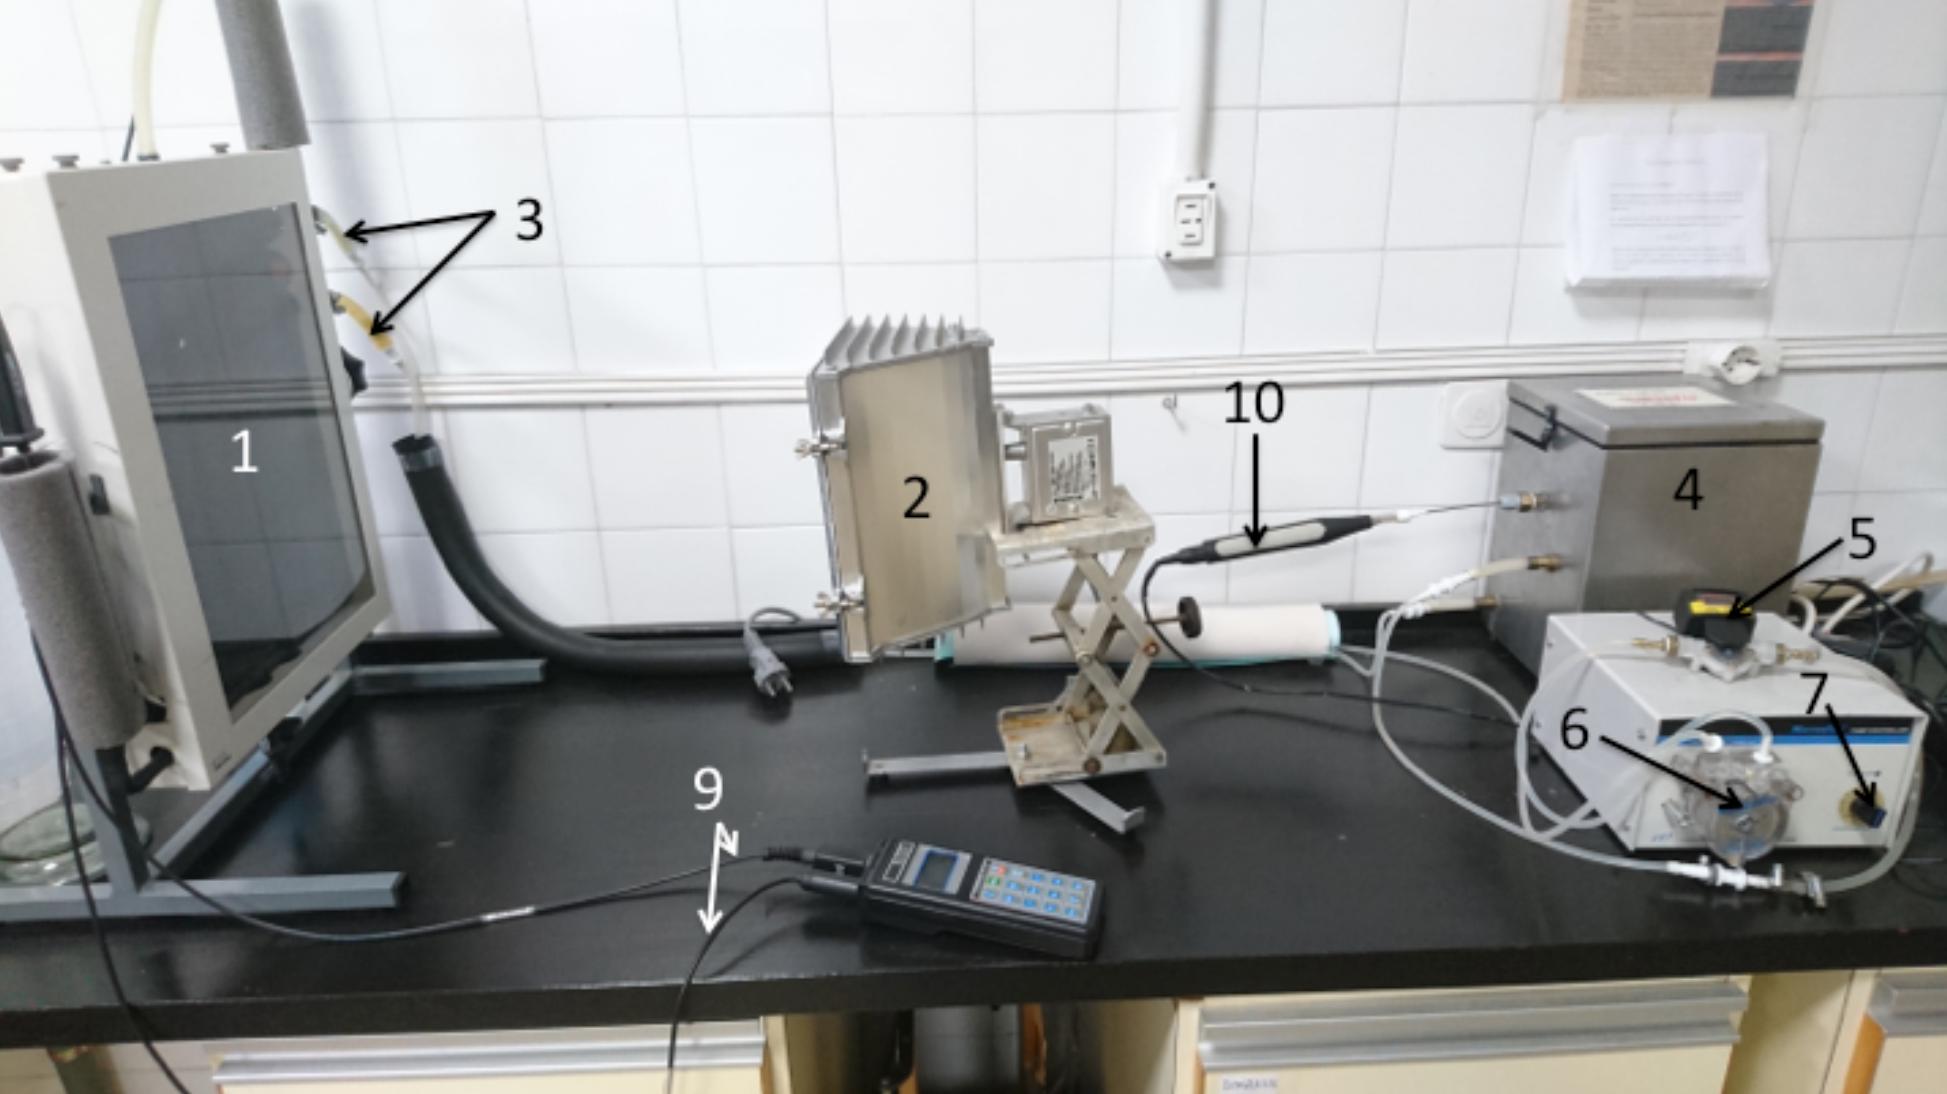
\includegraphics[scale=0.5]{dispositivo_experimantal.png}
\caption{montaje experimental}
\end{figure}

Donde cada número va asociado a un elemento en el apartado material. De todos modos en la foto aparece la bomba peristáltica vieja, que se ha renovado recientemente. Lo que representamos en (6) ahora mismo se ve tal y como en la figura 2. \\

\begin{figure}[h!] \centering
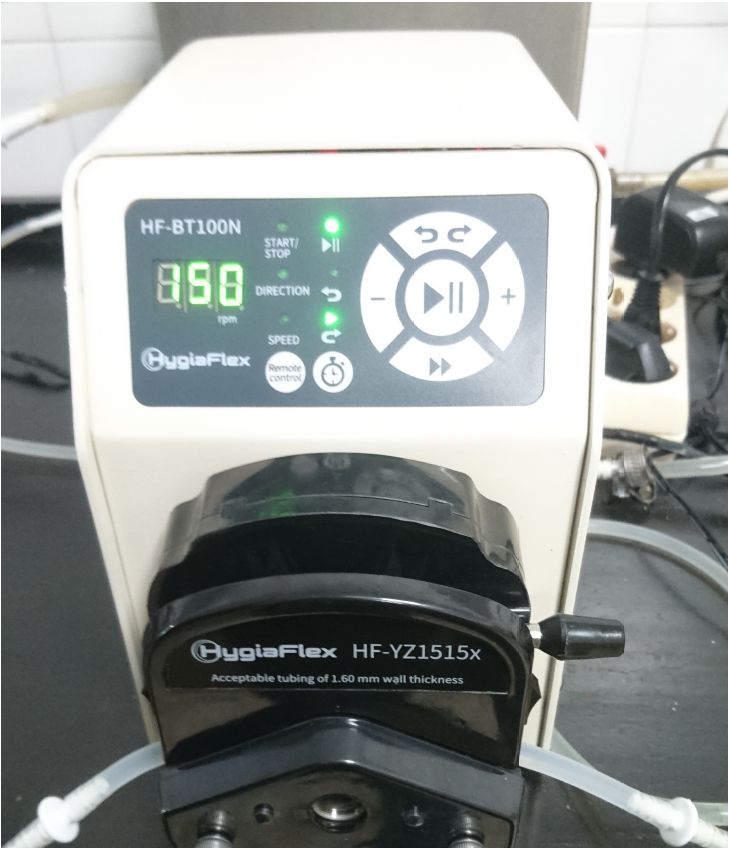
\includegraphics[scale=0.5]{bomba.png}
\label{Fig:1}
\caption{nueva bomba peristáltica}
\end{figure}

Entonces una vez tenemos el montaje listo podemos comenzar. Lo primero que vamos a tener que hacer es colocar a la distancia correcta la placa solar. Esto lo haremos ayudándonos de un metro y probablemente de nuestro compañero, ya que es un poco complicado medir la distancia correctamente. Una vez tengamos la distancia correcta, trataremos de poner el foco lo mas paralelo a la superficie de la placa, así como centrado. También mediremos con una regla o el metro la longitud de los lados de nuestra placa para conocer su superficie. Una vez tengamos todo esto, podemos encender el foco y la bomba. \\

Como ya mencionamos brevemente en la parte teórica, trataremos de buscar el estado estacionario de nuestro sistema, para cierto caudal y distancia fija. En este caso llamamos estado estacionario a el estado en el que la energía intercambiada en cada proceso sea constante. Esto se traducirá a que la diferencia de temperaturas $\Delta T$ y lo que aumenta por unidad de tiempo la temperatura $T_3$ sea constante, dado que la masa, la capacidad calorifica, la distancia y el caudal permanecerán, idealmente constantes. Digo idealmente porque cabe la posibilidad de que el caudal cambie a lo largo del tiempo por diversas razones. \\

Estaremos en el estado estacionario cuando la $\Delta T$ permanezca constante a lo largo de 2-3 minutos. A uno se le podría ocurrir que por qué no usar también la $\Delta T_3/\Delta t$, pero usar esto podría inducir a un error, ya que el foco de incertidumbre de $T_3$ es bastante grande. Quiero decir, en cada momento dicho valor dado por el termómetro oscila bastante (ya lo trataremos mejor en la sección de incertidumbres), y pretender que no varíe es muy complicado.  \\

Una vez lleguemos al estado estacionario mediremos $\Delta T$ (comprobando varias veces que se mantiene constante) y el caudal $Q$. Además realizaremos un estudio de la evolución temporal de $T_3$. Como en el estado estacionario  sabemos que lo que varía la temperatura por unidad de tiempo es la misma, por lo que podemos suponer un comportamiento lineal:

\begin{equation}
T_3 = a + b t
\end{equation}

teniendo entonces que $\D T_3 / \D t = b$. Por lo tanto tomaremos pares de valores ($t,T_3$) a lo largo de dos minutos (cada 15 segundos aproximadamente) para luego hacer la regresión lineal y obtener dicho valor para el estado estacionario. \\

Una vez hayamos acabado dicho proceso tendremos que cambiar el caudal, y si ya hemos hecho todos los caudales de una distancia, cambiar la distancia. La primera distancia que usaremos entre foco y placa será de 75 cm, luego probaremos con 50 cm. Ahora vamos a ver cuales caudales vamos a usar. Lo que vamos a hacer en está práctica será seleccionar las revoluciones por minuto de nuestra bomba, y con esas revoluciones ver que caudal da. Las revoluciones que vamos a usar serán 120, 90, 60 y 40. Deberíamos poder bajar a 30, pero, al menos en nuestro caso, no pudimos, siendo el mínimo 40 r.p.m. las que podíamos seleccionar. También hay algo llamativo. En función de la distancia a la placa, para las mismas revoluciones dan diferentes caudales. Ejemplificando, si seleccionas 150 r.p.m. para la distancia 75 cm y 50 cm tenemos que los caudales serán de 149 ml/min y 152 ml/min. Nosotros lo que hicimos fue seleccionar los mismos r.p.m que la anterior, pero eso llevo a unas pequeñas diferencias en los caudales. Quizás en la segunda vez habría que ajustar las revoluciones para que queden los mismos caudales, y hacer la comparación. 



\section{Propagación de incertidumbres}
En esta sección escribimos las fórmulas de la propagación de incertidumbres.  Obviamente los valores tabulados ($c_p,m_{d}\ldots$) no se tienen en cuenta a la hora de calcular la propagación de incertidumbres.

\begin{equation}
s(S) = s(L) \cdot \parentesis{L_1^2 + L_2^2}^{1/2}
\end{equation}

\begin{equation}
s(I) = \dfrac{2 \cdot 247.24}{d^3} s(d)
\end{equation}

\begin{equation}
s(E_1) = \ccorchetes{S^2 \cdot s^2(I) + I^2 \cdot s^2(S)}^{1/2}
\end{equation}


\begin{equation}
s(E_2) = \ccorchetes{ (c_p \Delta T)^2 s^2(Q)+(c_p Q) s^2(\Delta T)}^{1/2}
\end{equation}

\begin{equation}
s(E_3) = (m_d C_p) \cdot s(b)
\end{equation}

\begin{equation}
s(\eta_1) = \ccorchetes{ \parentesis{\dfrac{E_2}{E_1^2}}^2 s^2(E_1) + \parentesis{\dfrac{1}{E_1}}^2 s^2(E_2) }^{1/2}
\end{equation}



\begin{equation}
s(\eta_2) = \ccorchetes{ \parentesis{\dfrac{E_3}{E_2^2}}^2 s^2(E_2) + \parentesis{\dfrac{1}{E_2}}^2 s^2(E_3) }^{1/2}
\end{equation}



\begin{equation}
s(\eta_3) = \ccorchetes{ \parentesis{\dfrac{E_3}{E_1^2}}^2 s^2(E_1) + \parentesis{\dfrac{1}{E_1}}^2 s^2(E_3) }^{1/2}
\end{equation}


\newpage

\section{Incertidumbres}

En esta sección vamos a estudiar las incertidumbres de todo nuestro proceso, una por una, las analizaremos, de la manera mas rigurosa posible. \\


Lo primero que vamos a estudiar es la incertidumbre de la temperatura tomada por los termometros. Un termómetro digital funciona con una distribución de frecuencias lineal, por lo que sabemos que una de las incertidumbres de tipo B de nuestros datos será $l/\sqrt{12}$, siendo $l$ la precisión del aparato. Otra incertidumbre de tipo B que podemos incluir será la incertidumbre especificada por los fabricantes. Por desgracia no fue posible conseguir la de uno de los termómetro que usamos, pero si que conocemos la especificación del termómetros. En general el fabricante del termómetro que nos da la diferencia de temperaturas (9), que es un Delta OHM HD 8706-R2, nos dice que el error es de $0.2C^o \pm 0.2\%$. Como no tenemos incertidumbre de tipo A ya que con este termómetro los valores no oscilan, tenemos entonces que las incertidumbres de $\Delta T$ variarán bastante. \\

La información del otro termómetro es nula, pero si podemos ver que, en general, oscila mucho, y es muy difícil tomar una medida exacta de $T_3$. Nosotros por eso le asignamos una incertidumbre de $0.2 C^o$, ya que generalmente oscilaba entre el valor dado y 0.02 grados centígrados. Considerar aquí la incertidumbre de la distribuciones de frecuencia no servíria de nada, ya que $0.02 >  0.01/\sqrt{12}$; por lo que escogeremos la primera como incertidumbre constante y para todos las medidas por igual. \\

\begin{equation}
s(T_3) = 0.2
\end{equation}

La incertidumbre del tiempo cuando tomamos los valores de $T_3$ es difícil de explicar. Como sabemos la precisión del aparato es de 0.01 s, pero la capacidad del humano para reaccionar es mayor (entorno a 1 segundo). Sin embargo, también es cierto que ya podemos ir observando la tendencia poco a poco del tiempo, donde realmente asignamos un valor con bastante precisión ya que segundos previos y posteriores al tiempo la temperatura se mantiene (aunque hay otras veces que no). De hecho, darle un valor de incertidumbre del tiempo se antoja un poco raro, mas que nada porque realmente hay muchos factores que influencian a esta toma de datos. Se antoja muy arbitraria y difícilmente decidible. Aun con todo creo que, aunque no sea de una manera concisa y rigurosa, la incertidumbre, teniendo en cuenta todo lo anterior, sera de 1 segundo. 

\begin{equation}
s(t) = 1 s
\end{equation}

La otra incertidumbre que nos queda por analizar es la del caudal. Como la toma de datos se hace con un aparato digital, ya conocemos la distribución de frecuencia, pero como con otras medidas, la oscilación que a veces tiene lugar nos hace asignarle un valor de incertidumbre de tipo B a mayores que será de 1 ml/min. Entonces la incertidumbre total será de:

\begin{equation}
s(Q) = \sqrt{1+1/12} = 1.0 ml/min
\end{equation}

Por tanto la incertidumbre final será la de la precisión del aparato, aunque a la hora de propagar de ml/min a g/s se tendrá en cuenta todo el valor.  \\



\newpage

\section{Resultados experimentales}



\subsection{Primera distancia}
 
\subsubsection{Caudal número 1} 
 
Usando los datos del apartado \ref{subsec:1} y los  resultados experimentales de la regreisón lineal (tab \ref{tab:regresion1}) (fig \ref{Fig:plot-1}), podemos calcular las energías 
 
 \begin{equation} 
\begin{array}{lllllll}
E_1 & = & 85.3 W &  \ \ &  s(E_1) & =  & 2.7  W \\ 
 E_2 & = & 67.8 W &  \ \ &  s(E_2) & =  & 3.5  W \\ 
 E_3 & = & 50.1 W &  \ \ &  s(E_3) & =  & 3.1  W \\ 
 \end{array} 
\end{equation} 
 
 y podemos calcular los rendimientos 
 
\begin{equation} 
\begin{array}{lllllll}
\eta_1 & = & 0.795  &  \ \ &  s(\eta_1) & =  & 0.048   \\ 
 \eta_2 & = & 0.740  &  \ \ &  s(\eta_2) & =  & 0.059   \\ 
 \eta_3 & = & 0.588  &  \ \ &  s(\eta_3) & =  & 0.041   \\ 
 \end{array} 
\end{equation} 
 
 \begin{table}[h!] 	 \centering 
\begin{tabular}{|c|c|c|c|} 
\hline 
$a \ (C^o)$ & $s(a) \ (C^o)$ & $ b \ (C^o/s)$ & $s(b) \ (C^o/s)$  \\ \hline 
19.035  & 0.012 &  0.001619 & 0.000099 \\ 
\hline
\end{tabular} 
\caption{Valores del ajuste lineal para los pares ($t,T_3$) con $Q=2.533 \ (g/s)$ y $d= 75 $ cm} 
\label{tab:regresion1} 
\end{table} 
 
 
\begin{figure}[h!] 	 \centering 
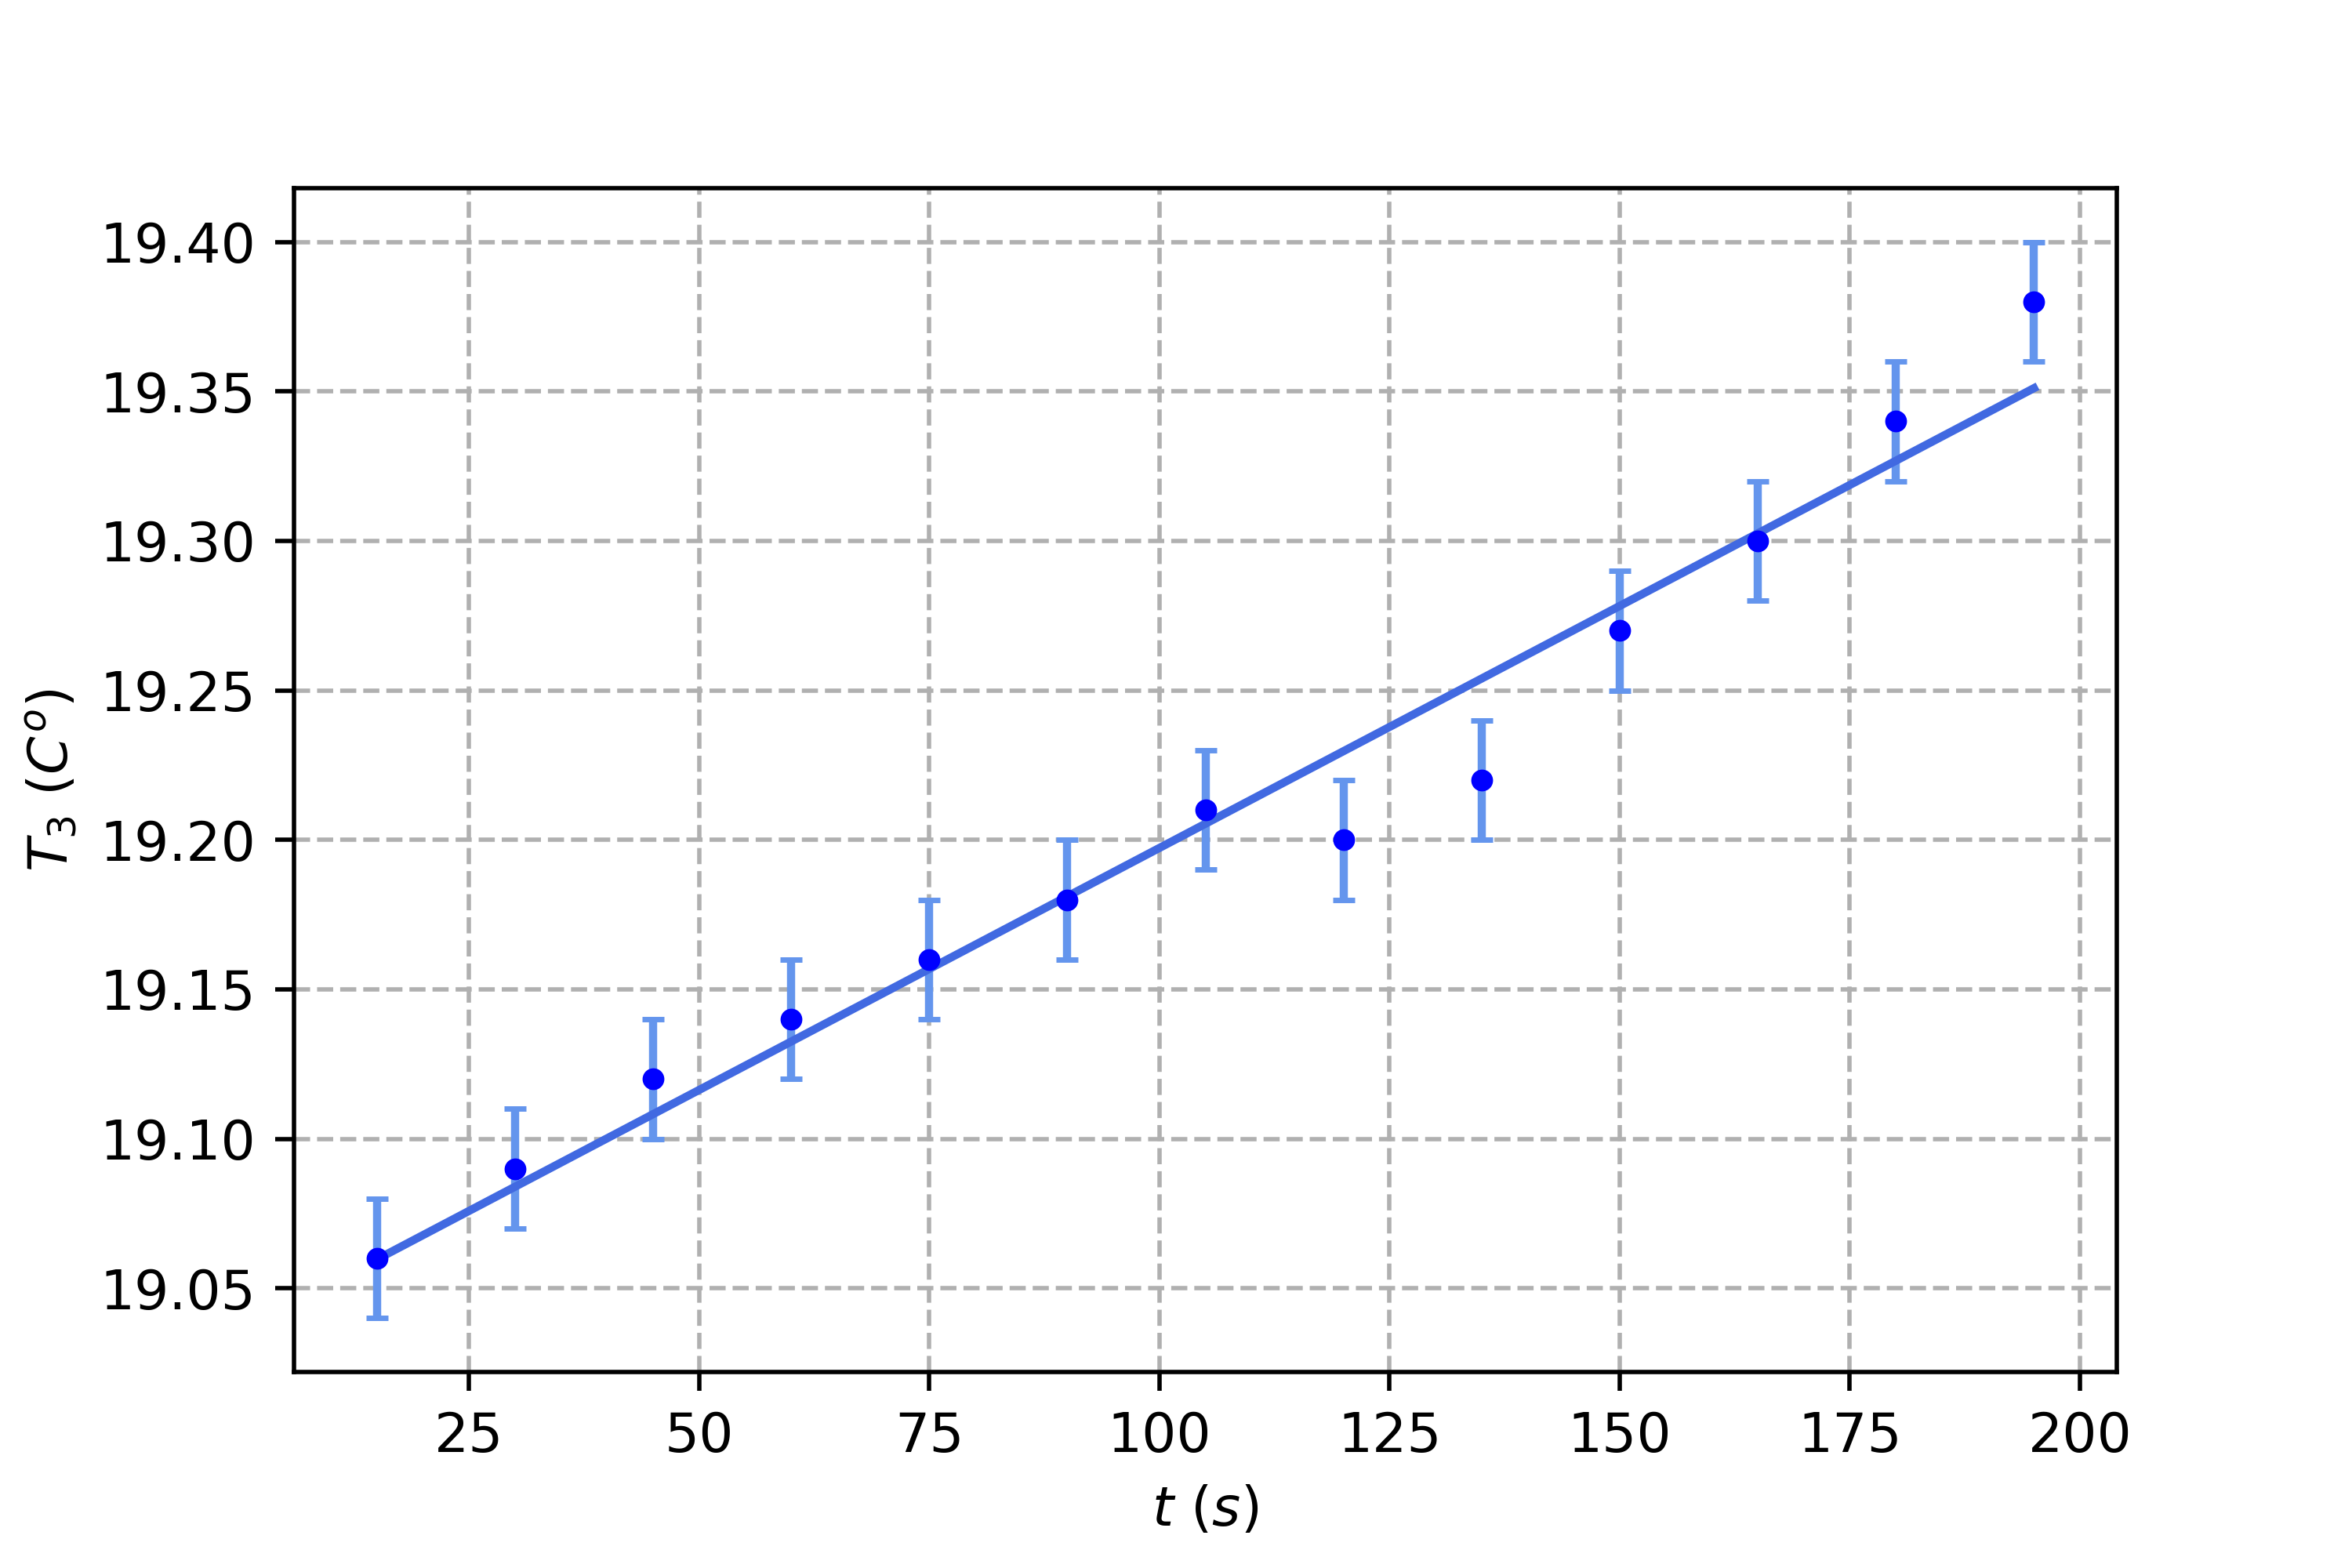
\includegraphics[scale=1.0]{plotT30.png} 
\caption{representación de $T_3$ frente a $t$ para $Q = 2.533 \ g/s$ e $d = 75$ cm} 
\label{Fig:plot-1}  
\end{figure} 
 
\newpage 
 
 
 
 
\subsubsection{Caudal número 2} 
 
Usando los datos del apartado \ref{subsec:2} y los  resultados experimentales de la regreisón lineal (tab \ref{tab:regresion2}) (fig \ref{Fig:plot-2}), podemos calcular las energías 
 
 \begin{equation} 
\begin{array}{lllllll}
E_1 & = & 85.3 W &  \ \ &  s(E_1) & =  & 2.7  W \\ 
 E_2 & = & 68.2 W &  \ \ &  s(E_2) & =  & 3.1  W \\ 
 E_3 & = & 53.7 W &  \ \ &  s(E_3) & =  & 3.1  W \\ 
 \end{array} 
\end{equation} 
 
 y podemos calcular los rendimientos 
 
\begin{equation} 
\begin{array}{lllllll}
\eta_1 & = & 0.800  &  \ \ &  s(\eta_1) & =  & 0.045   \\ 
 \eta_2 & = & 0.786  &  \ \ &  s(\eta_2) & =  & 0.058   \\ 
 \eta_3 & = & 0.629  &  \ \ &  s(\eta_3) & =  & 0.041   \\ 
 \end{array} 
\end{equation} 
 
 \begin{table}[h!] 	 \centering 
\begin{tabular}{|c|c|c|c|} 
\hline 
$a \ (C^o)$ & $s(a) \ (C^o)$ & $ b \ (C^o/s)$ & $s(b) \ (C^o/s)$  \\ \hline 
20.638  & 0.012 &  0.001733 & 0.000099 \\ 
\hline
\end{tabular} 
\caption{Valores del ajuste lineal para los pares ($t,T_3$) con $Q=2.067 \ (g/s)$ y $d= 75 $ cm} 
\label{tab:regresion2} 
\end{table} 
 
 
\begin{figure}[h!] 	 \centering 
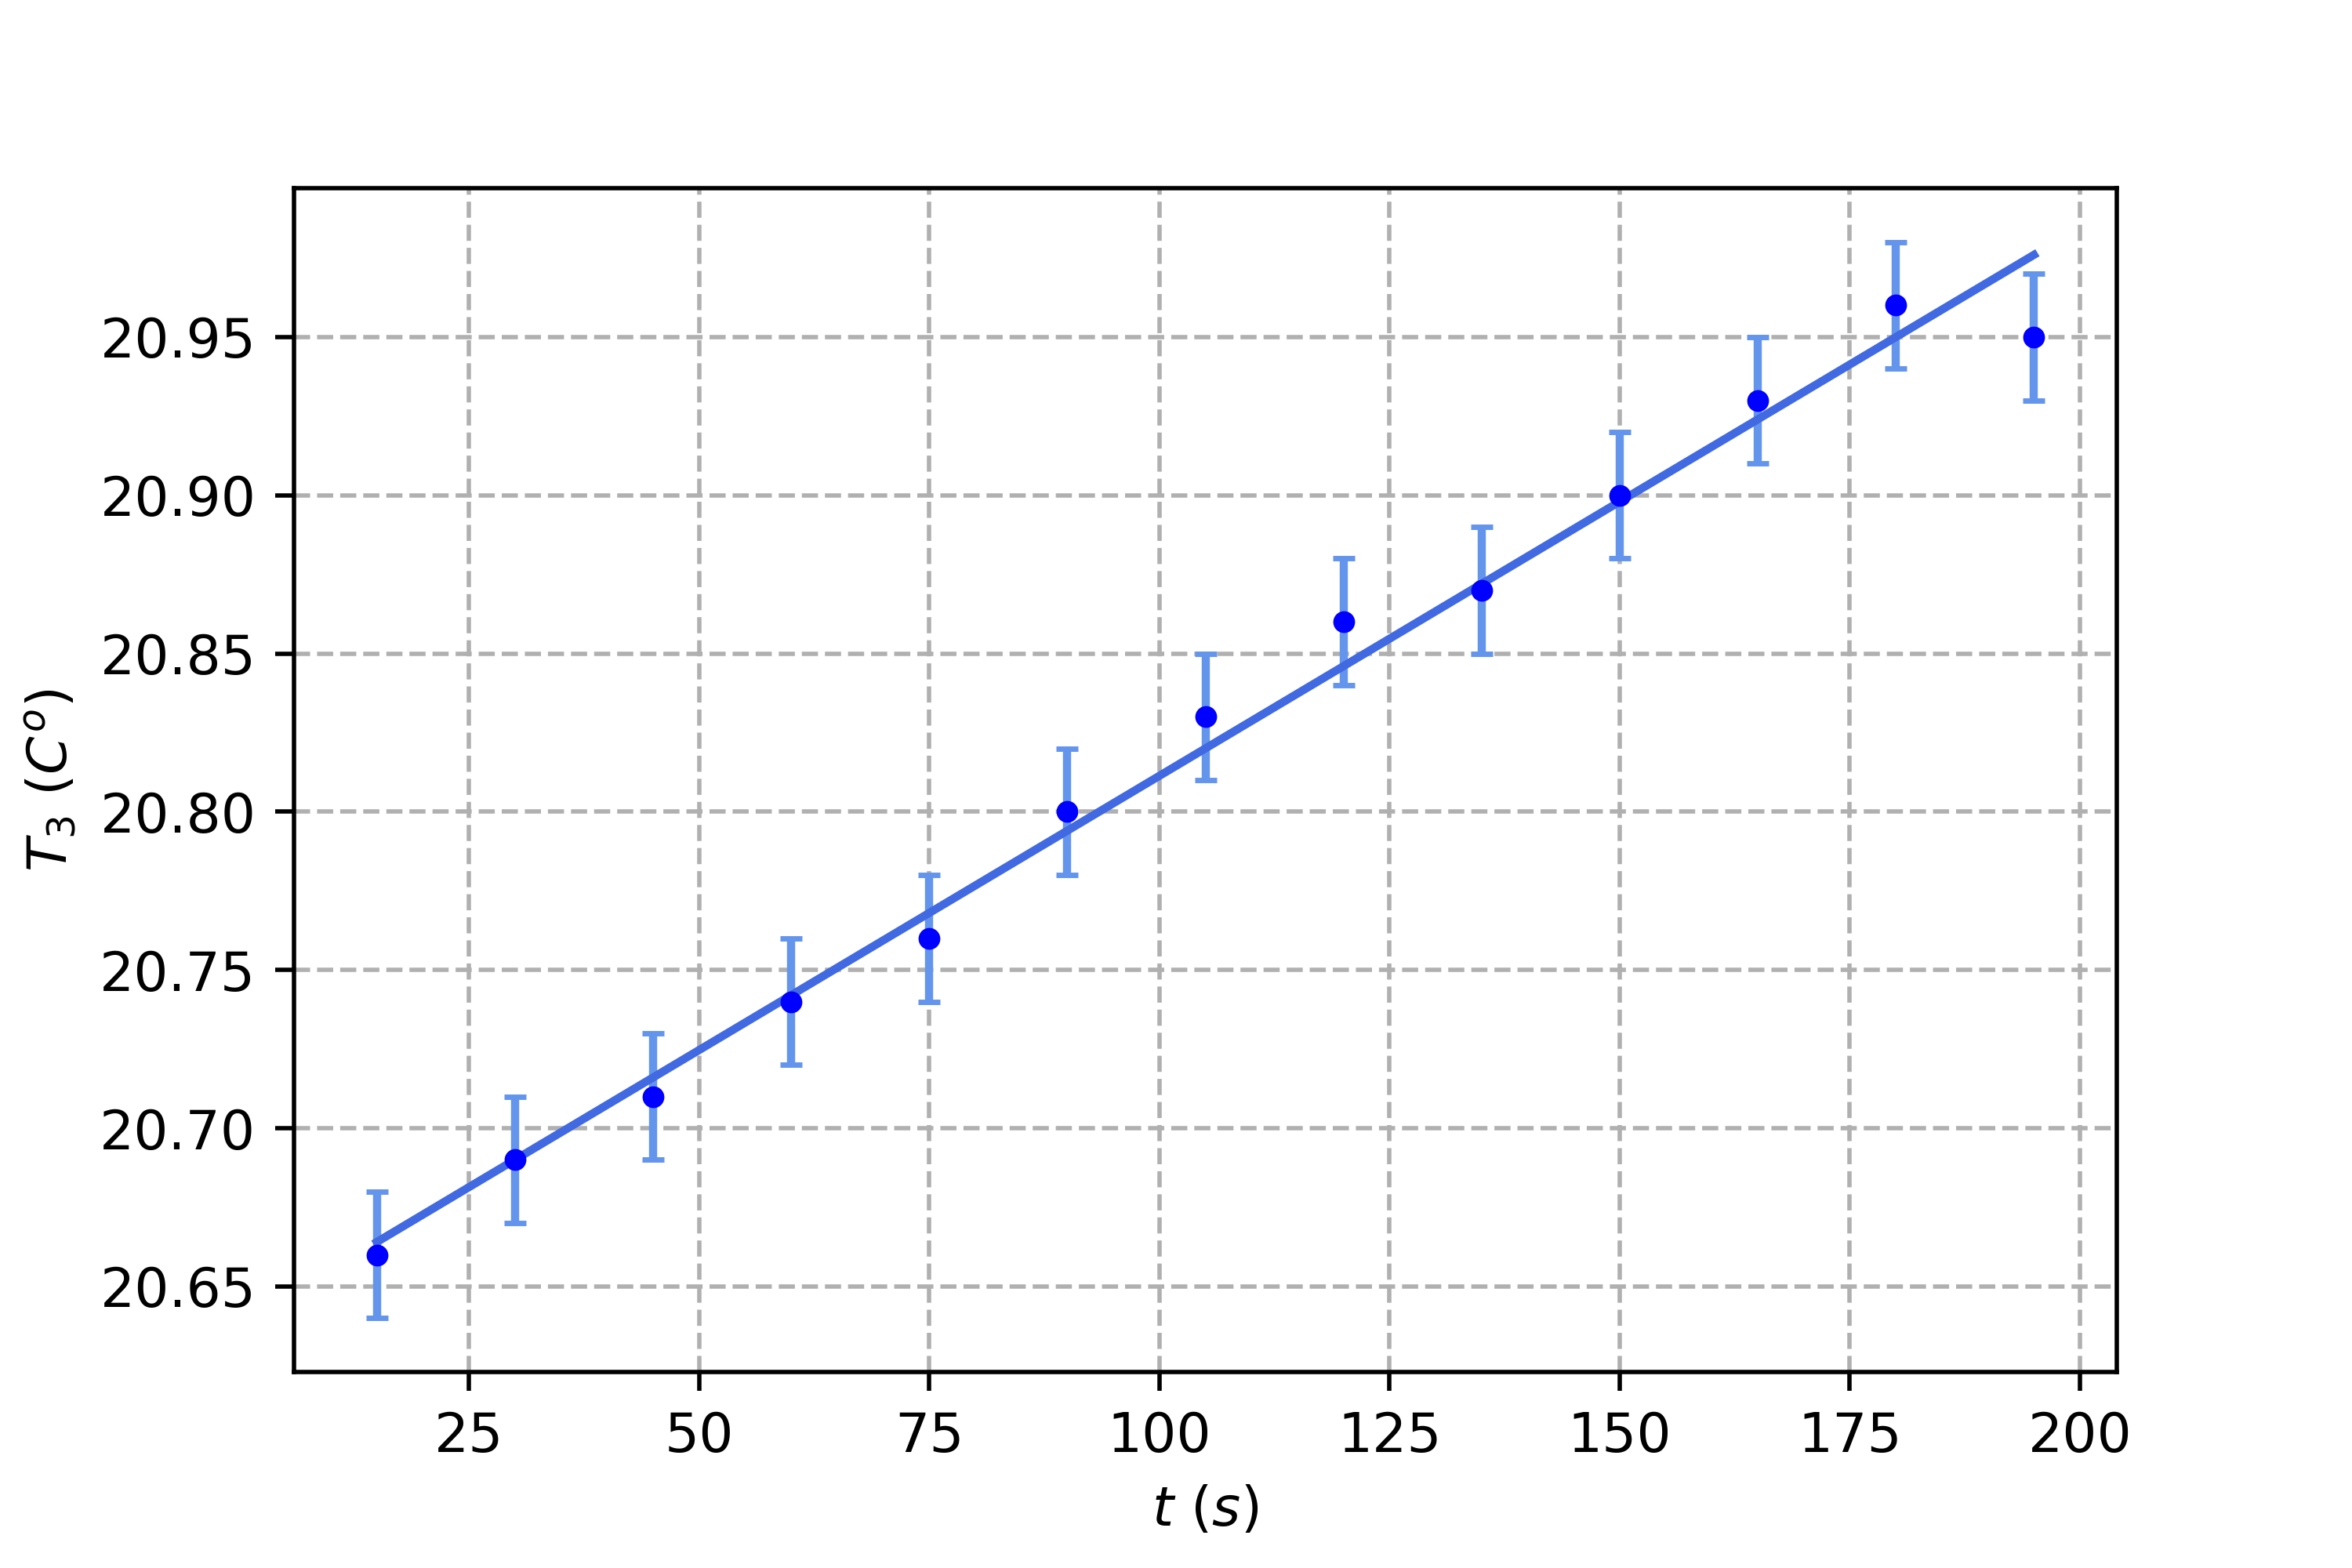
\includegraphics[scale=1.0]{plotT31.png} 
\caption{representación de $T_3$ frente a $t$ para $Q = 2.067 \ g/s$ e $d = 75$ cm} 
\label{Fig:plot-2}  
\end{figure} 
 
\newpage 
 
 
 
 
\subsubsection{Caudal número 3} 
 
Usando los datos del apartado \ref{subsec:3} y los  resultados experimentales de la regreisón lineal (tab \ref{tab:regresion3}) (fig \ref{Fig:plot-3}), podemos calcular las energías 
 
 \begin{equation} 
\begin{array}{lllllll}
E_1 & = & 85.3 W &  \ \ &  s(E_1) & =  & 2.7  W \\ 
 E_2 & = & 66.2 W &  \ \ &  s(E_2) & =  & 2.8  W \\ 
 E_3 & = & 48.0 W &  \ \ &  s(E_3) & =  & 3.5  W \\ 
 \end{array} 
\end{equation} 
 
 y podemos calcular los rendimientos 
 
\begin{equation} 
\begin{array}{lllllll}
\eta_1 & = & 0.777  &  \ \ &  s(\eta_1) & =  & 0.041   \\ 
 \eta_2 & = & 0.725  &  \ \ &  s(\eta_2) & =  & 0.060   \\ 
 \eta_3 & = & 0.563  &  \ \ &  s(\eta_3) & =  & 0.044   \\ 
 \end{array} 
\end{equation} 
 
 \begin{table}[h!] 	 \centering 
\begin{tabular}{|c|c|c|c|} 
\hline 
$a \ (C^o)$ & $s(a) \ (C^o)$ & $ b \ (C^o/s)$ & $s(b) \ (C^o/s)$  \\ \hline 
22.418  & 0.011 &  0.00155 & 0.00011 \\ 
\hline
\end{tabular} 
\caption{Valores del ajuste lineal para los pares ($t,T_3$) con $Q=1.633 \ (g/s)$ y $d= 75 $ cm} 
\label{tab:regresion3} 
\end{table} 
 
 
\begin{figure}[h!] 	 \centering 
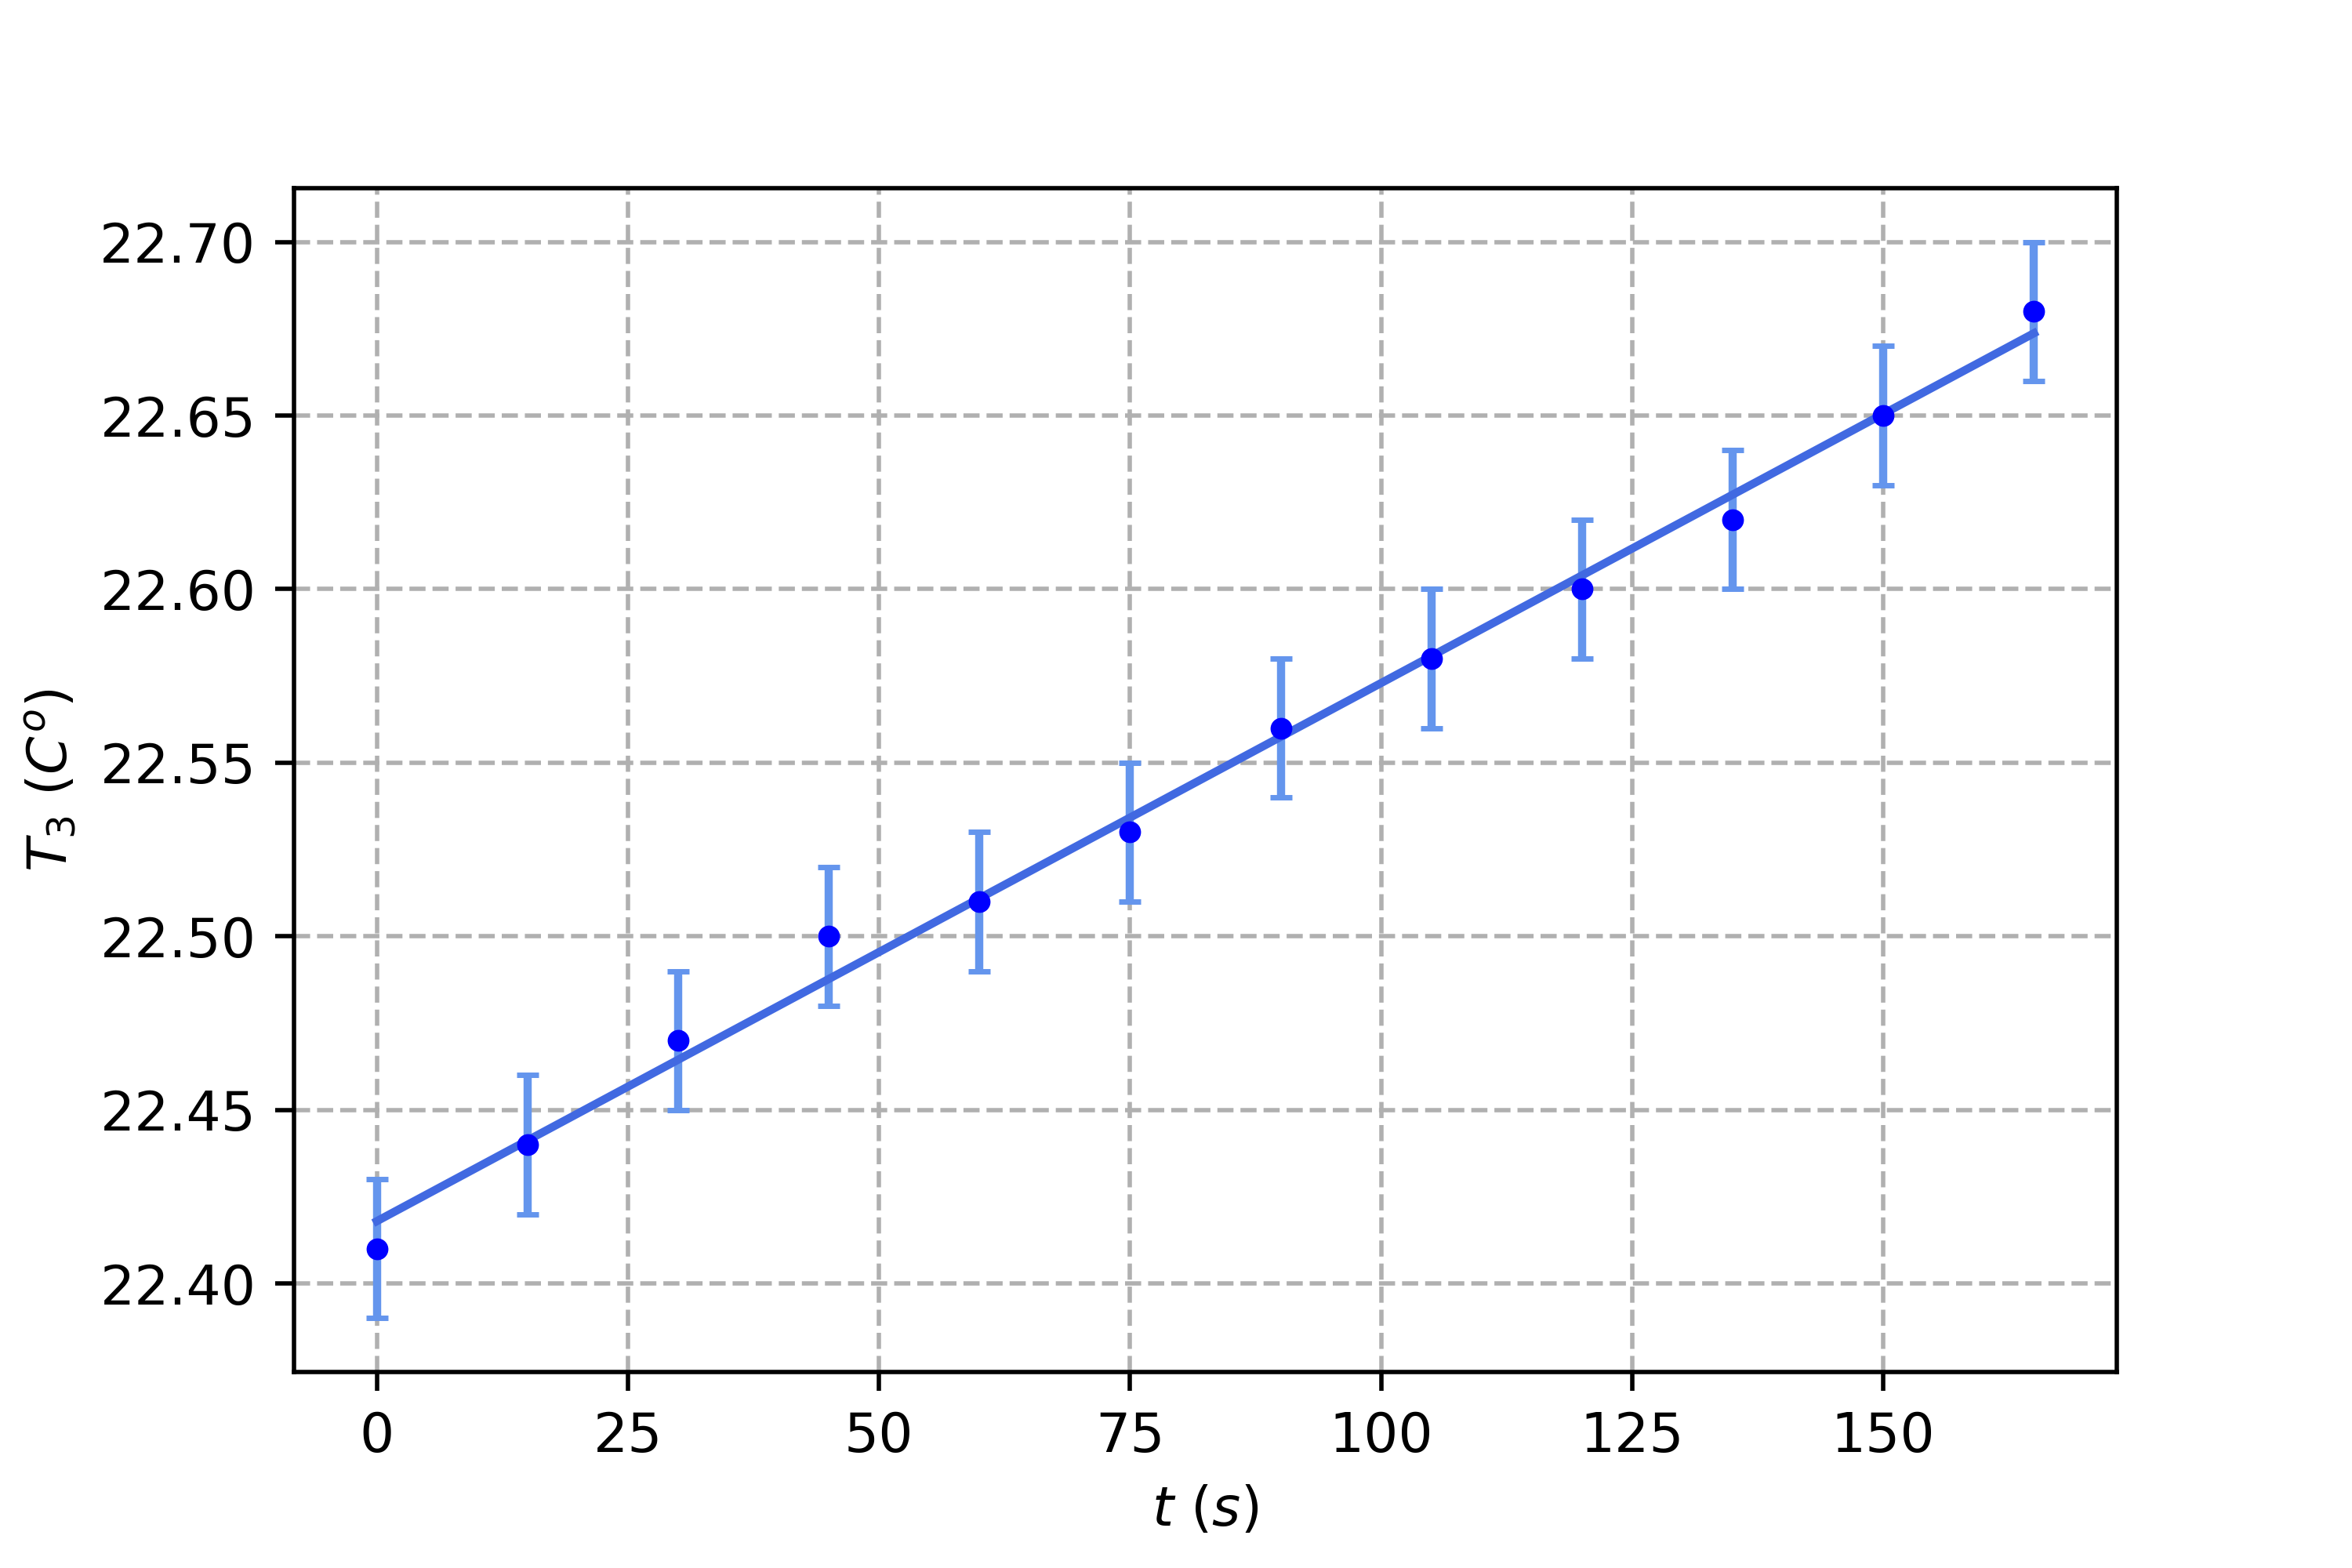
\includegraphics[scale=1.0]{plotT32.png} 
\caption{representación de $T_3$ frente a $t$ para $Q = 1.633 \ g/s$ e $d = 75$ cm} 
\label{Fig:plot-3}  
\end{figure} 
 
\newpage 
 
 
 
 
\subsubsection{Caudal número 4} 
 
Usando los datos del apartado \ref{subsec:4} y los  resultados experimentales de la regreisón lineal (tab \ref{tab:regresion4}) (fig \ref{Fig:plot-4}), podemos calcular las energías 
 
 \begin{equation} 
\begin{array}{lllllll}
E_1 & = & 85.3 W &  \ \ &  s(E_1) & =  & 2.7  W \\ 
 E_2 & = & 63.5 W &  \ \ &  s(E_2) & =  & 2.4  W \\ 
 E_3 & = & 34.2 W &  \ \ &  s(E_3) & =  & 3.1  W \\ 
 \end{array} 
\end{equation} 
 
 y podemos calcular los rendimientos 
 
\begin{equation} 
\begin{array}{lllllll}
\eta_1 & = & 0.744  &  \ \ &  s(\eta_1) & =  & 0.037   \\ 
 \eta_2 & = & 0.538  &  \ \ &  s(\eta_2) & =  & 0.052   \\ 
 \eta_3 & = & 0.400  &  \ \ &  s(\eta_3) & =  & 0.038   \\ 
 \end{array} 
\end{equation} 
 
 \begin{table}[h!] 	 \centering 
\begin{tabular}{|c|c|c|c|} 
\hline 
$a \ (C^o)$ & $s(a) \ (C^o)$ & $ b \ (C^o/s)$ & $s(b) \ (C^o/s)$  \\ \hline 
23.645  & 0.010 &  0.001103 & 0.000099 \\ 
\hline
\end{tabular} 
\caption{Valores del ajuste lineal para los pares ($t,T_3$) con $Q=1.150 \ (g/s)$ y $d= 75 $ cm} 
\label{tab:regresion4} 
\end{table} 
 
 
\begin{figure}[h!] 	 \centering 
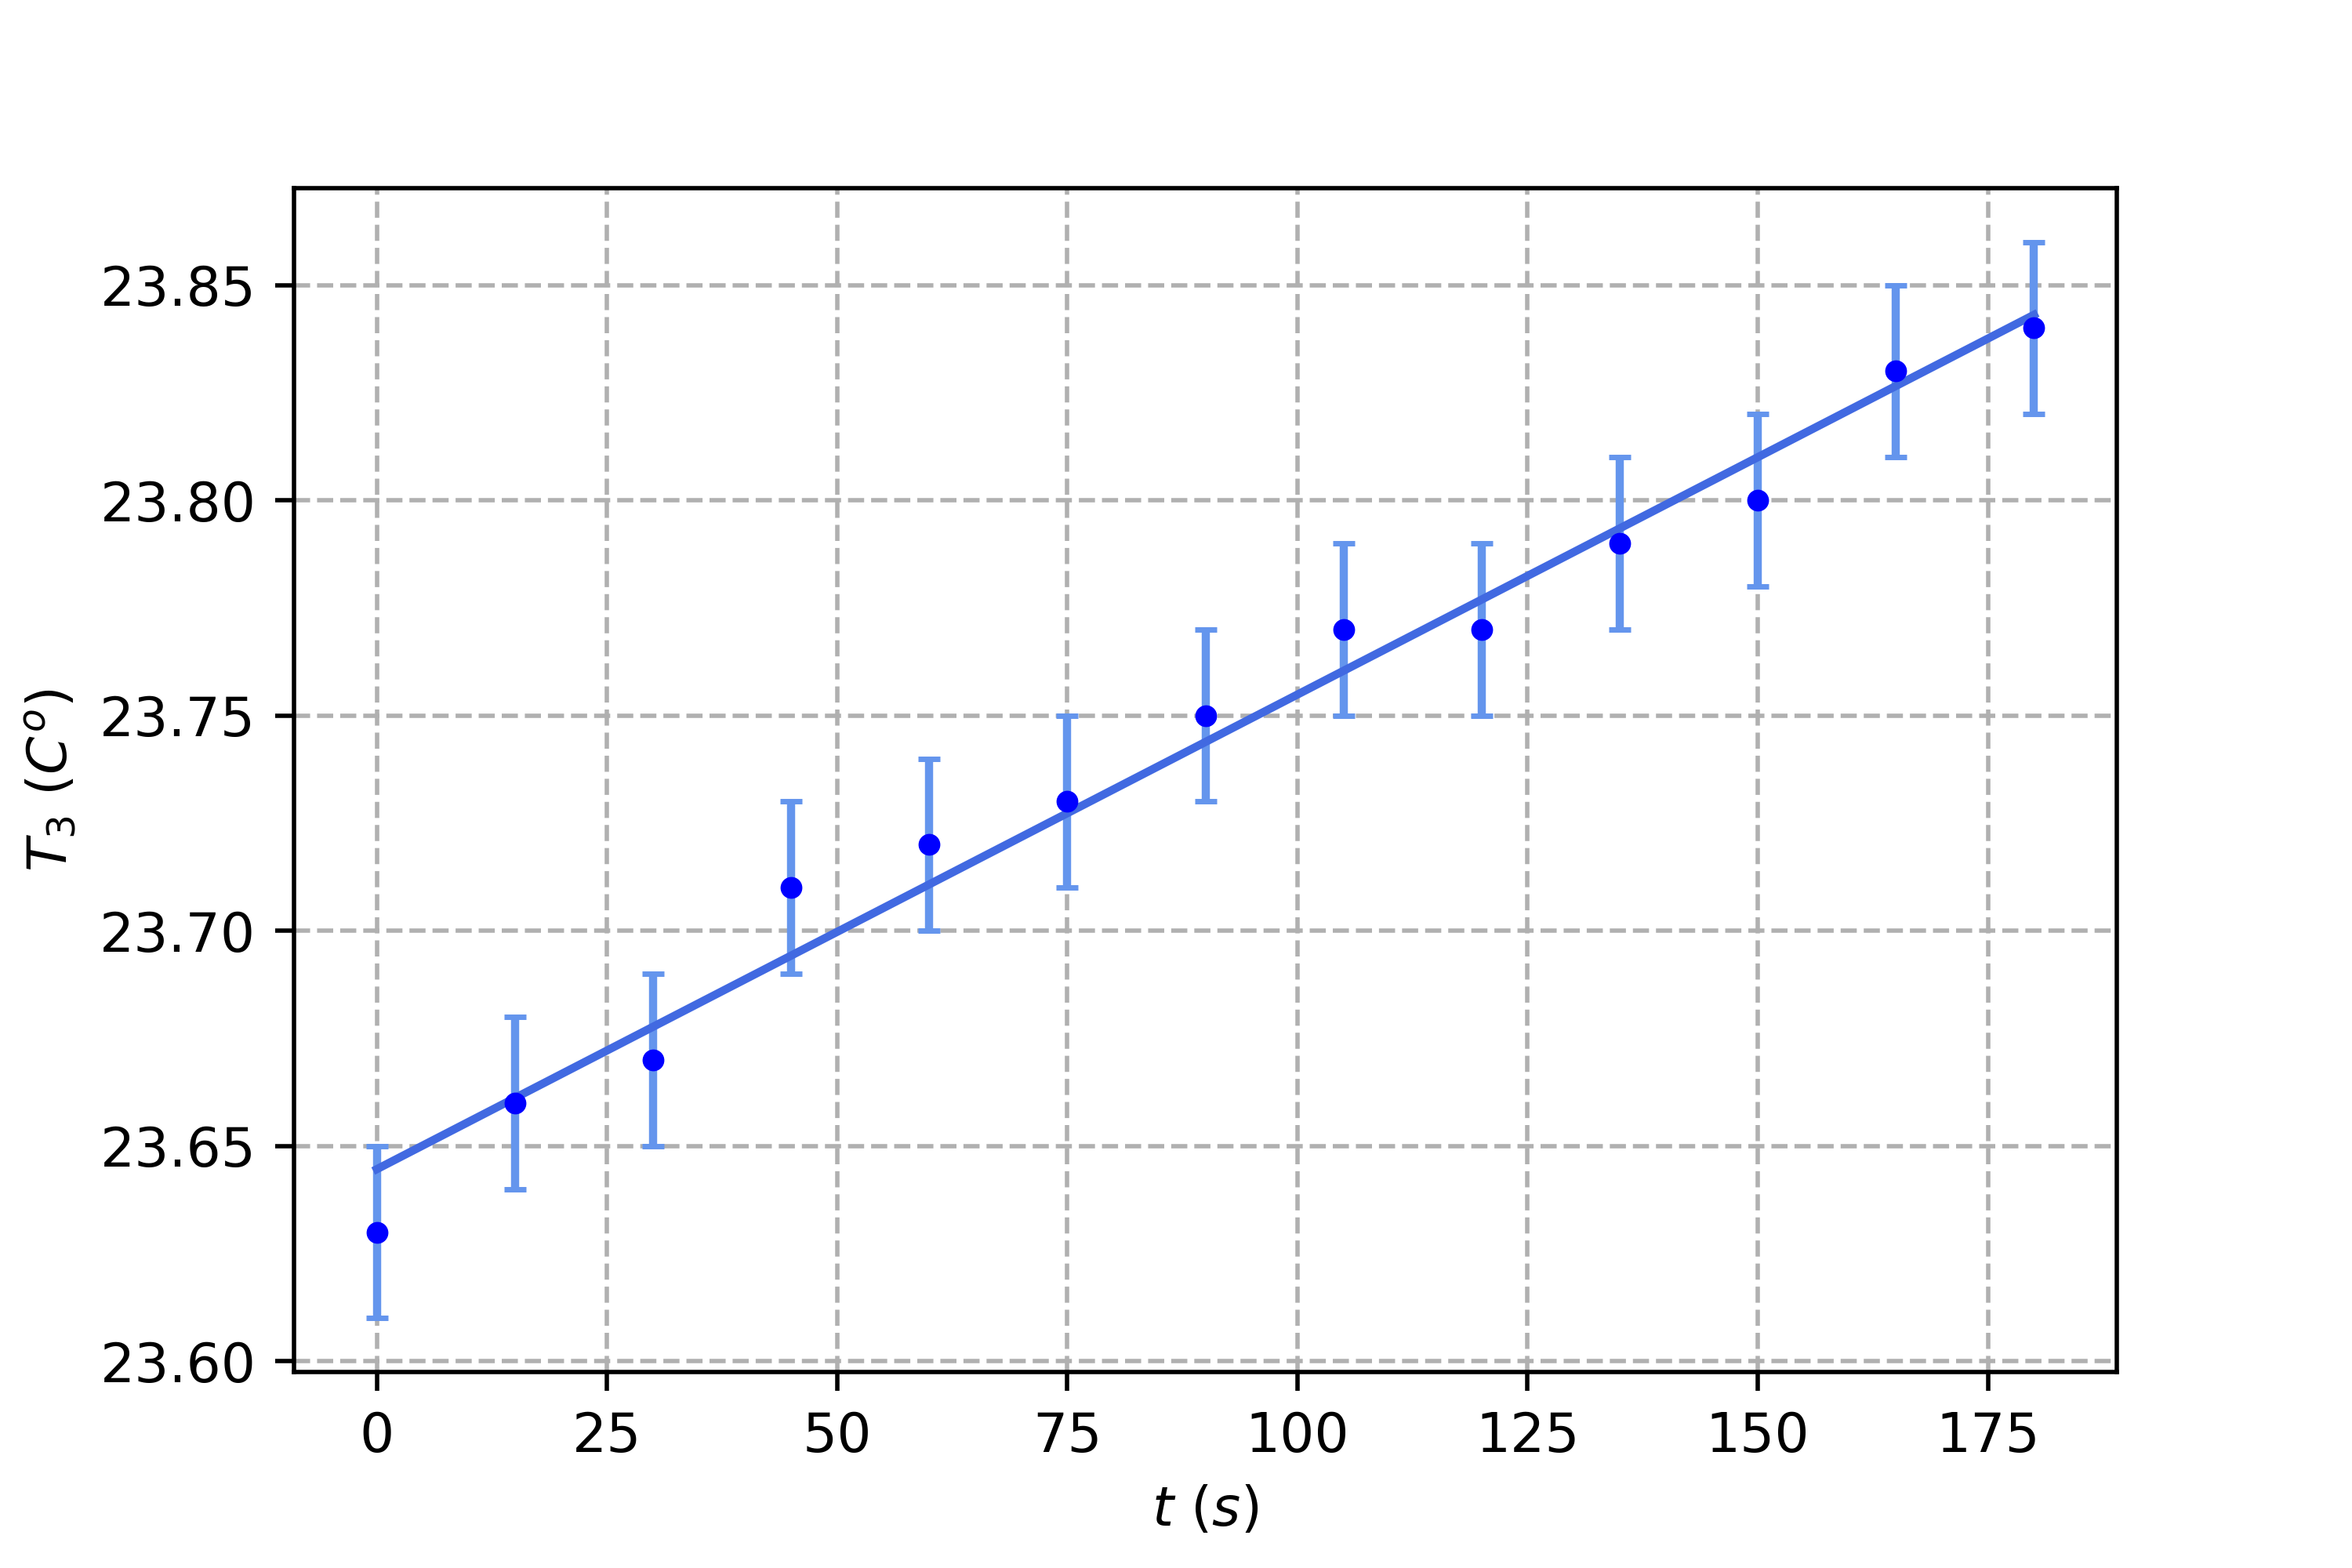
\includegraphics[scale=1.0]{plotT33.png} 
\caption{representación de $T_3$ frente a $t$ para $Q = 1.150 \ g/s$ e $d = 75$ cm} 
\label{Fig:plot-4}  
\end{figure} 
 
\newpage 
 
 
 
 
\subsubsection{Caudal número 5} 
 
Usando los datos del apartado \ref{subsec:5} y los  resultados experimentales de la regreisón lineal (tab \ref{tab:regresion5}) (fig \ref{Fig:plot-5}), podemos calcular las energías 
 
 \begin{equation} 
\begin{array}{lllllll}
E_1 & = & 85.3 W &  \ \ &  s(E_1) & =  & 2.7  W \\ 
 E_2 & = & 61.1 W &  \ \ &  s(E_2) & =  & 2.3  W \\ 
 E_3 & = & 32.9 W &  \ \ &  s(E_3) & =  & 3.5  W \\ 
 \end{array} 
\end{equation} 
 
 y podemos calcular los rendimientos 
 
\begin{equation} 
\begin{array}{lllllll}
\eta_1 & = & 0.717  &  \ \ &  s(\eta_1) & =  & 0.035   \\ 
 \eta_2 & = & 0.539  &  \ \ &  s(\eta_2) & =  & 0.060   \\ 
 \eta_3 & = & 0.386  &  \ \ &  s(\eta_3) & =  & 0.042   \\ 
 \end{array} 
\end{equation} 
 
 \begin{table}[h!] 	 \centering 
\begin{tabular}{|c|c|c|c|} 
\hline 
$a \ (C^o)$ & $s(a) \ (C^o)$ & $ b \ (C^o/s)$ & $s(b) \ (C^o/s)$  \\ \hline 
24.797  & 0.011 &  0.00106 & 0.00011 \\ 
\hline
\end{tabular} 
\caption{Valores del ajuste lineal para los pares ($t,T_3$) con $Q=0.817 \ (g/s)$ y $d= 75 $ cm} 
\label{tab:regresion5} 
\end{table} 
 
 
\begin{figure}[h!] 	 \centering 
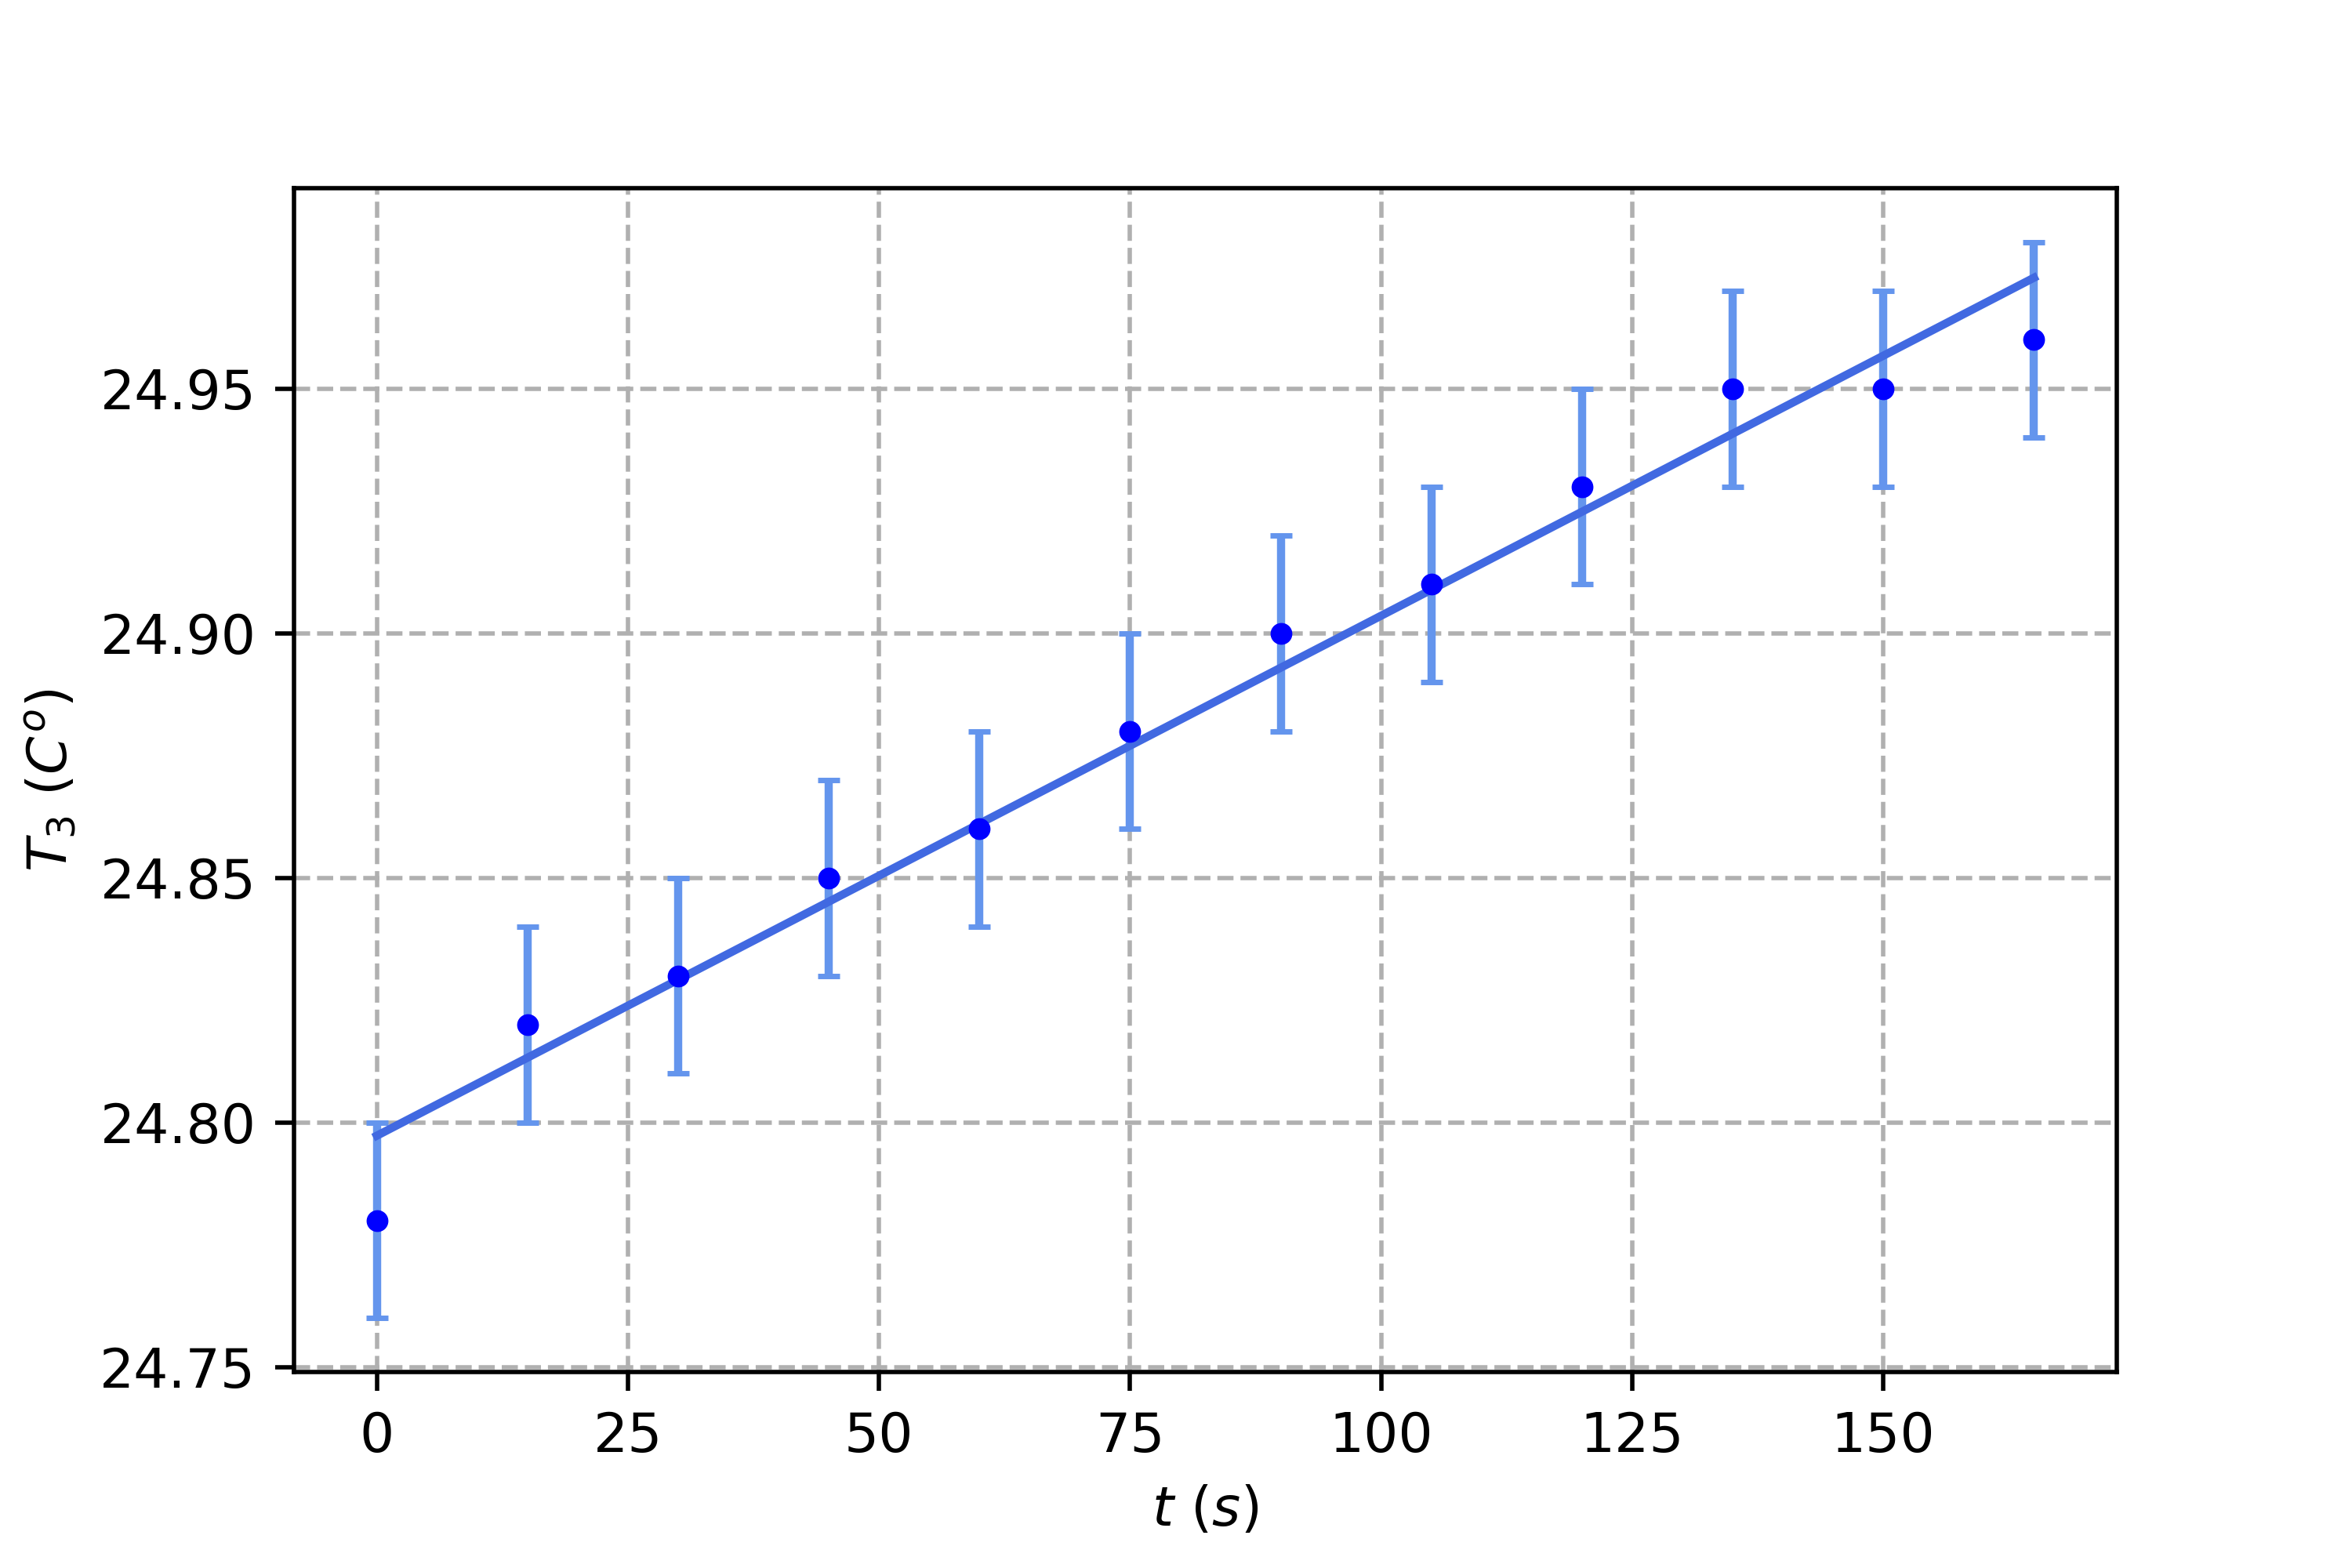
\includegraphics[scale=1.0]{plotT34.png} 
\caption{representación de $T_3$ frente a $t$ para $Q = 0.817 \ g/s$ e $d = 75$ cm} 
\label{Fig:plot-5}  
\end{figure} 
 
\newpage 
 
 
 
 
\subsection{Segunda distancia}
\subsubsection{Caudal número 1} 
 
Usando los datos del apartado \ref{subsec:6} y los  resultados experimentales de la regreisón lineal (tab \ref{tab:regresion6}) (fig \ref{Fig:plot-6}), podemos calcular las energías 
 
 \begin{equation} 
\begin{array}{lllllll}
E_1 & = & 146.6 W &  \ \ &  s(E_1) & =  & 8.9  W \\ 
 E_2 & = & 105.5 W &  \ \ &  s(E_2) & =  & 4.3  W \\ 
 E_3 & = & 85.5 W &  \ \ &  s(E_3) & =  & 3.2  W \\ 
 \end{array} 
\end{equation} 
 
 y podemos calcular los rendimientos 
 
\begin{equation} 
\begin{array}{lllllll}
\eta_1 & = & 0.720  &  \ \ &  s(\eta_1) & =  & 0.053   \\ 
 \eta_2 & = & 0.810  &  \ \ &  s(\eta_2) & =  & 0.045   \\ 
 \eta_3 & = & 0.583  &  \ \ &  s(\eta_3) & =  & 0.042   \\ 
 \end{array} 
\end{equation} 
 
 \begin{table}[h!] 	 \centering 
\begin{tabular}{|c|c|c|c|} 
\hline 
$a \ (C^o)$ & $s(a) \ (C^o)$ & $ b \ (C^o/s)$ & $s(b) \ (C^o/s)$  \\ \hline 
20.092  & 0.011 &  0.00276 & 0.00010 \\ 
\hline
\end{tabular} 
\caption{Valores del ajuste lineal para los pares ($t,T_3$) con $Q=2.550 \ (g/s)$ y $d= 50 $ cm} 
\label{tab:regresion6} 
\end{table} 
 
 
\begin{figure}[h!] 	 \centering 
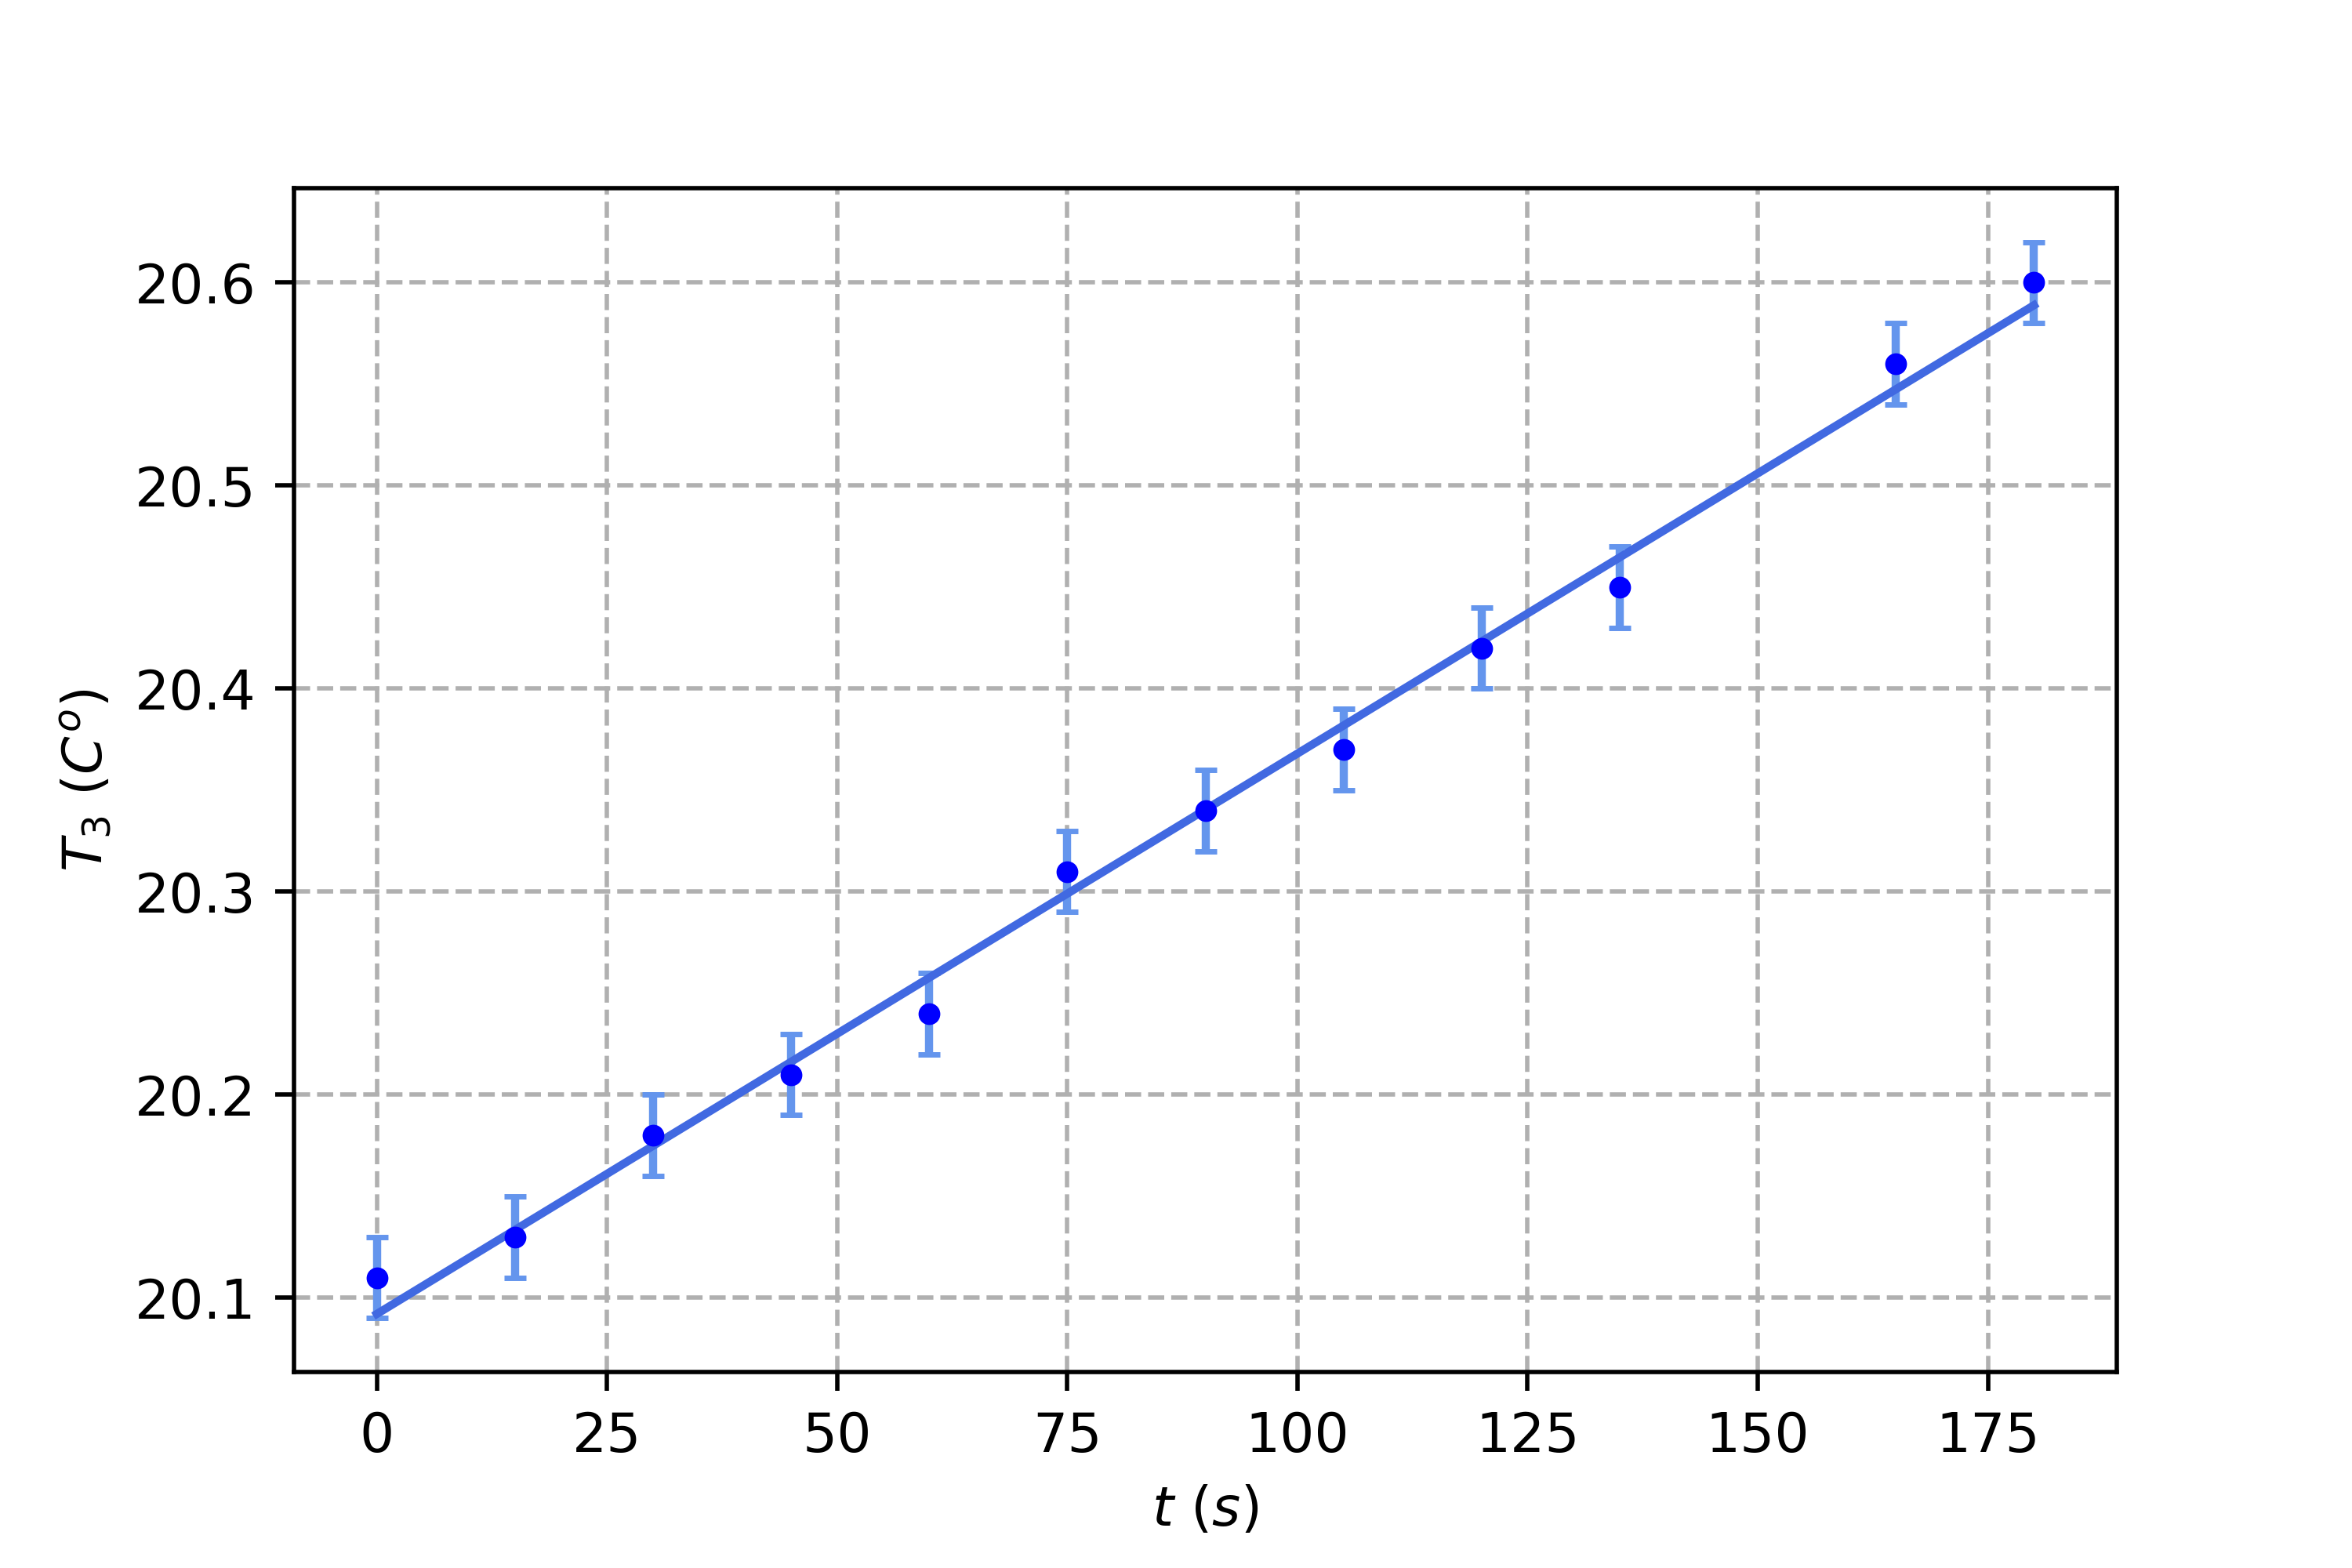
\includegraphics[scale=1.0]{plotT35.png} 
\caption{representación de $T_3$ frente a $t$ para $Q = 2.550 \ g/s$ e $d = 50$ cm} 
\label{Fig:plot-6}  
\end{figure} 
 
\newpage 
 
 
 
 
\subsubsection{Caudal número 2} 
 
Usando los datos del apartado \ref{subsec:7} y los  resultados experimentales de la regreisón lineal (tab \ref{tab:regresion7}) (fig \ref{Fig:plot-7}), podemos calcular las energías 
 
 \begin{equation} 
\begin{array}{lllllll}
E_1 & = & 146.6 W &  \ \ &  s(E_1) & =  & 8.9  W \\ 
 E_2 & = & 117.7 W &  \ \ &  s(E_2) & =  & 4.2  W \\ 
 E_3 & = & 66.7 W &  \ \ &  s(E_3) & =  & 3.1  W \\ 
 \end{array} 
\end{equation} 
 
 y podemos calcular los rendimientos 
 
\begin{equation} 
\begin{array}{lllllll}
\eta_1 & = & 0.803  &  \ \ &  s(\eta_1) & =  & 0.057   \\ 
 \eta_2 & = & 0.567  &  \ \ &  s(\eta_2) & =  & 0.033   \\ 
 \eta_3 & = & 0.455  &  \ \ &  s(\eta_3) & =  & 0.035   \\ 
 \end{array} 
\end{equation} 
 
 \begin{table}[h!] 	 \centering 
\begin{tabular}{|c|c|c|c|} 
\hline 
$a \ (C^o)$ & $s(a) \ (C^o)$ & $ b \ (C^o/s)$ & $s(b) \ (C^o/s)$  \\ \hline 
23.519  & 0.010 &  0.002154 & 0.000099 \\ 
\hline
\end{tabular} 
\caption{Valores del ajuste lineal para los pares ($t,T_3$) con $Q=2.117 \ (g/s)$ y $d= 50 $ cm} 
\label{tab:regresion7} 
\end{table} 
 
 
\begin{figure}[h!] 	 \centering 
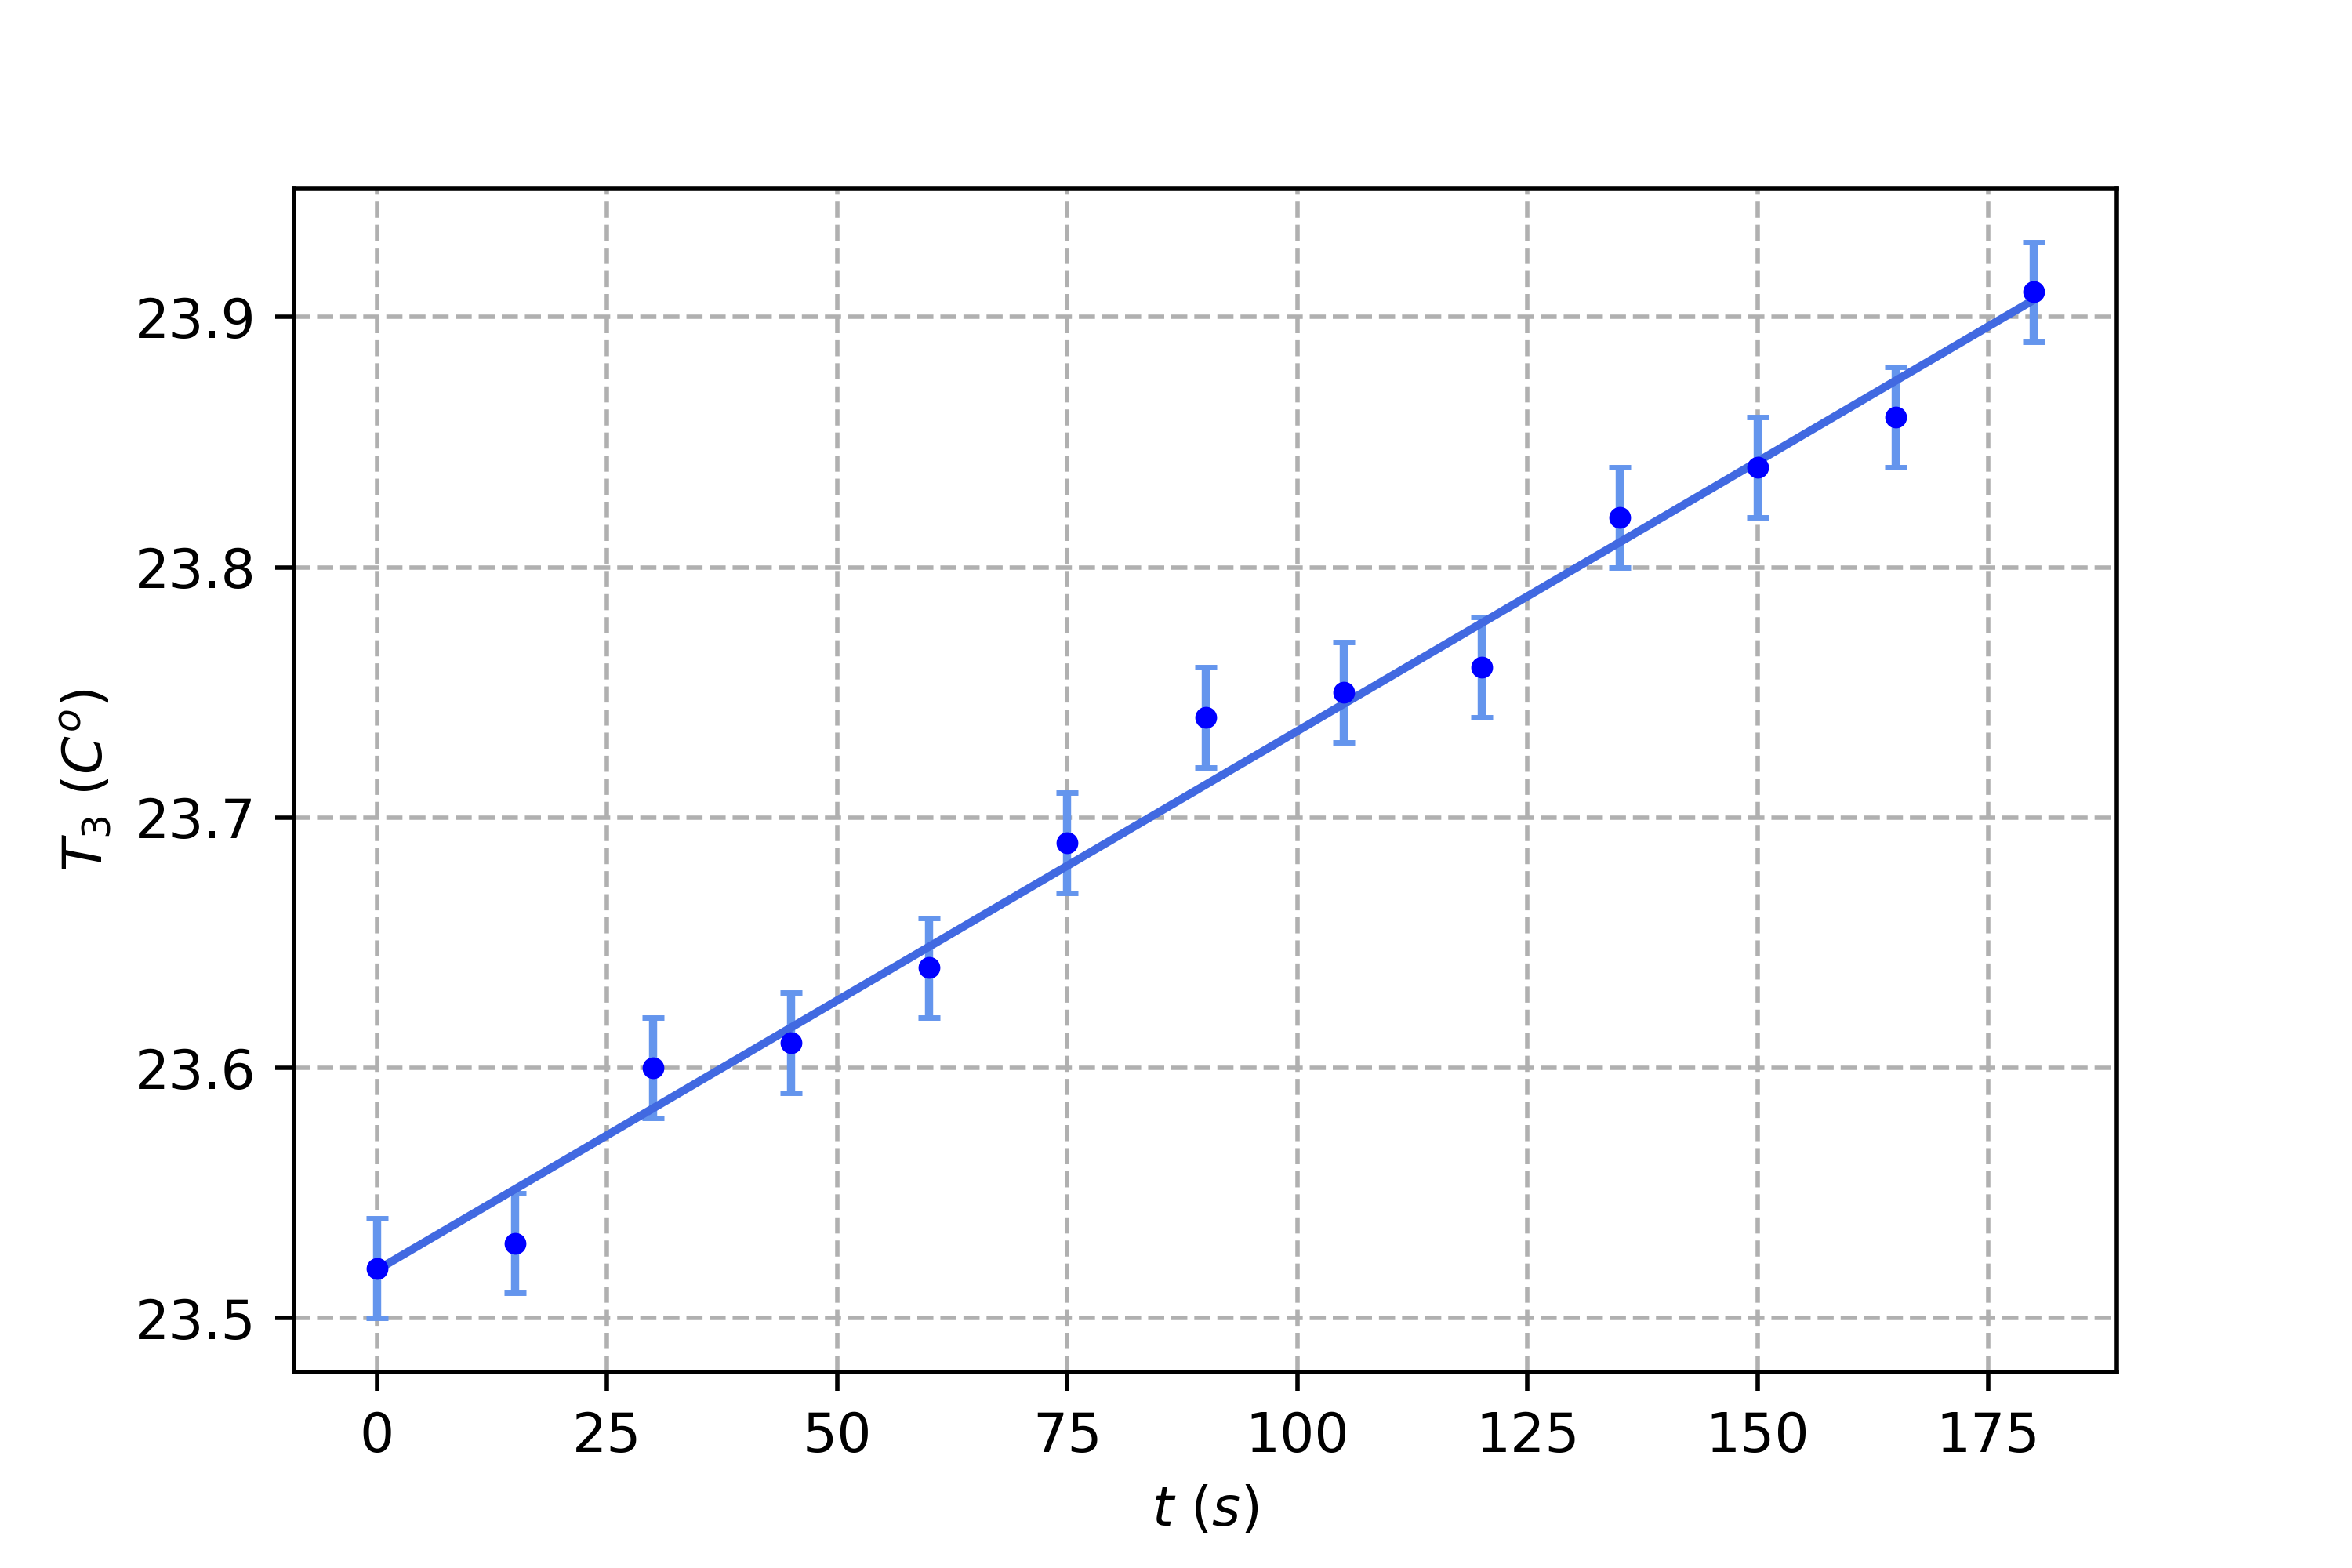
\includegraphics[scale=1.0]{plotT36.png} 
\caption{representación de $T_3$ frente a $t$ para $Q = 2.117 \ g/s$ e $d = 50$ cm} 
\label{Fig:plot-7}  
\end{figure} 
 
\newpage 
 
 
 
 
\subsubsection{Caudal número 3} 
 
Usando los datos del apartado \ref{subsec:8} y los  resultados experimentales de la regreisón lineal (tab \ref{tab:regresion8}) (fig \ref{Fig:plot-8}), podemos calcular las energías 
 
 \begin{equation} 
\begin{array}{lllllll}
E_1 & = & 146.6 W &  \ \ &  s(E_1) & =  & 8.9  W \\ 
 E_2 & = & 103.8 W &  \ \ &  s(E_2) & =  & 3.6  W \\ 
 E_3 & = & 65.0 W &  \ \ &  s(E_3) & =  & 3.1  W \\ 
 \end{array} 
\end{equation} 
 
 y podemos calcular los rendimientos 
 
\begin{equation} 
\begin{array}{lllllll}
\eta_1 & = & 0.708  &  \ \ &  s(\eta_1) & =  & 0.050   \\ 
 \eta_2 & = & 0.626  &  \ \ &  s(\eta_2) & =  & 0.037   \\ 
 \eta_3 & = & 0.443  &  \ \ &  s(\eta_3) & =  & 0.034   \\ 
 \end{array} 
\end{equation} 
 
 \begin{table}[h!] 	 \centering 
\begin{tabular}{|c|c|c|c|} 
\hline 
$a \ (C^o)$ & $s(a) \ (C^o)$ & $ b \ (C^o/s)$ & $s(b) \ (C^o/s)$  \\ \hline 
26.122  & 0.010 &  0.00210 & 0.00010 \\ 
\hline
\end{tabular} 
\caption{Valores del ajuste lineal para los pares ($t,T_3$) con $Q=1.667 \ (g/s)$ y $d= 50 $ cm} 
\label{tab:regresion8} 
\end{table} 
 
 
\begin{figure}[h!] 	 \centering 
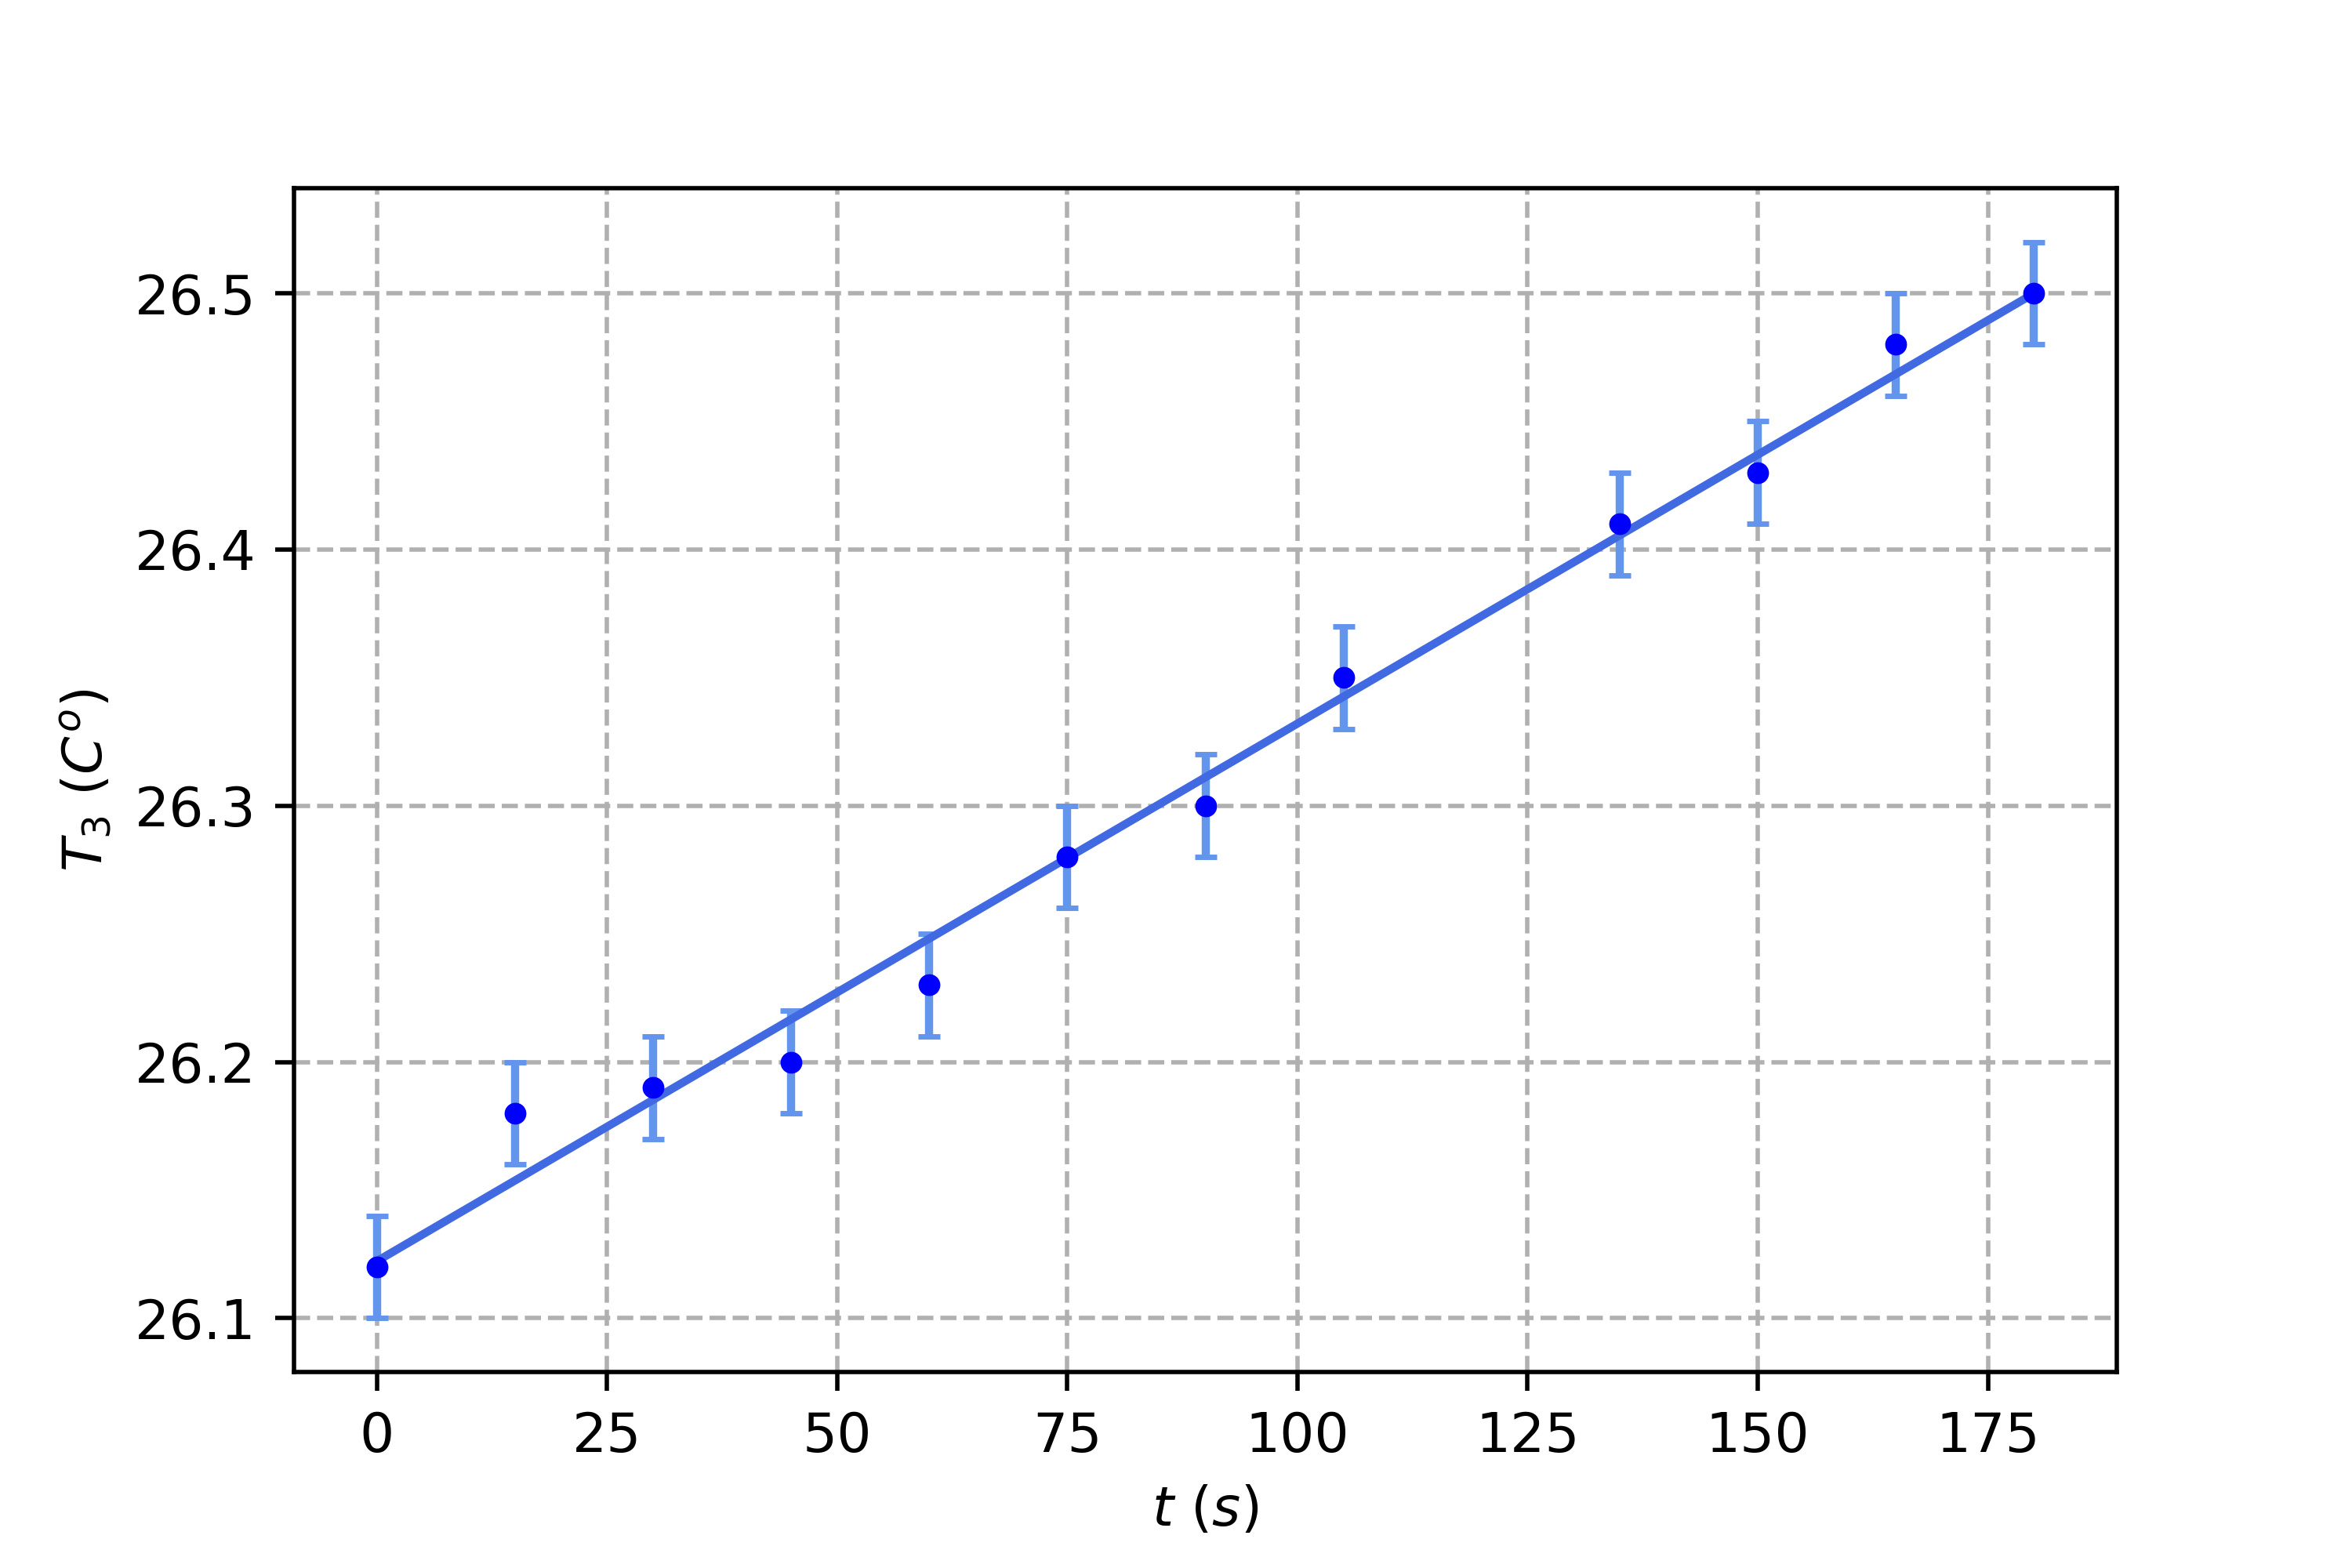
\includegraphics[scale=1.0]{plotT37.png} 
\caption{representación de $T_3$ frente a $t$ para $Q = 1.667 \ g/s$ e $d = 50$ cm} 
\label{Fig:plot-8}  
\end{figure} 
 
\newpage 
 
 
 
 
\subsubsection{Caudal número 4} 
 
Usando los datos del apartado \ref{subsec:9} y los  resultados experimentales de la regreisón lineal (tab \ref{tab:regresion9}) (fig \ref{Fig:plot-9}), podemos calcular las energías 
 
 \begin{equation} 
\begin{array}{lllllll}
E_1 & = & 146.6 W &  \ \ &  s(E_1) & =  & 8.9  W \\ 
 E_2 & = & 89.2 W &  \ \ &  s(E_2) & =  & 3.1  W \\ 
 E_3 & = & 57.9 W &  \ \ &  s(E_3) & =  & 3.6  W \\ 
 \end{array} 
\end{equation} 
 
 y podemos calcular los rendimientos 
 
\begin{equation} 
\begin{array}{lllllll}
\eta_1 & = & 0.609  &  \ \ &  s(\eta_1) & =  & 0.043   \\ 
 \eta_2 & = & 0.648  &  \ \ &  s(\eta_2) & =  & 0.046   \\ 
 \eta_3 & = & 0.395  &  \ \ &  s(\eta_3) & =  & 0.034   \\ 
 \end{array} 
\end{equation} 
 
 \begin{table}[h!] 	 \centering 
\begin{tabular}{|c|c|c|c|} 
\hline 
$a \ (C^o)$ & $s(a) \ (C^o)$ & $ b \ (C^o/s)$ & $s(b) \ (C^o/s)$  \\ \hline 
27.898  & 0.011 &  0.00187 & 0.00012 \\ 
\hline
\end{tabular} 
\caption{Valores del ajuste lineal para los pares ($t,T_3$) con $Q=1.167 \ (g/s)$ y $d= 50 $ cm} 
\label{tab:regresion9} 
\end{table} 
 
 
\begin{figure}[h!] 	 \centering 
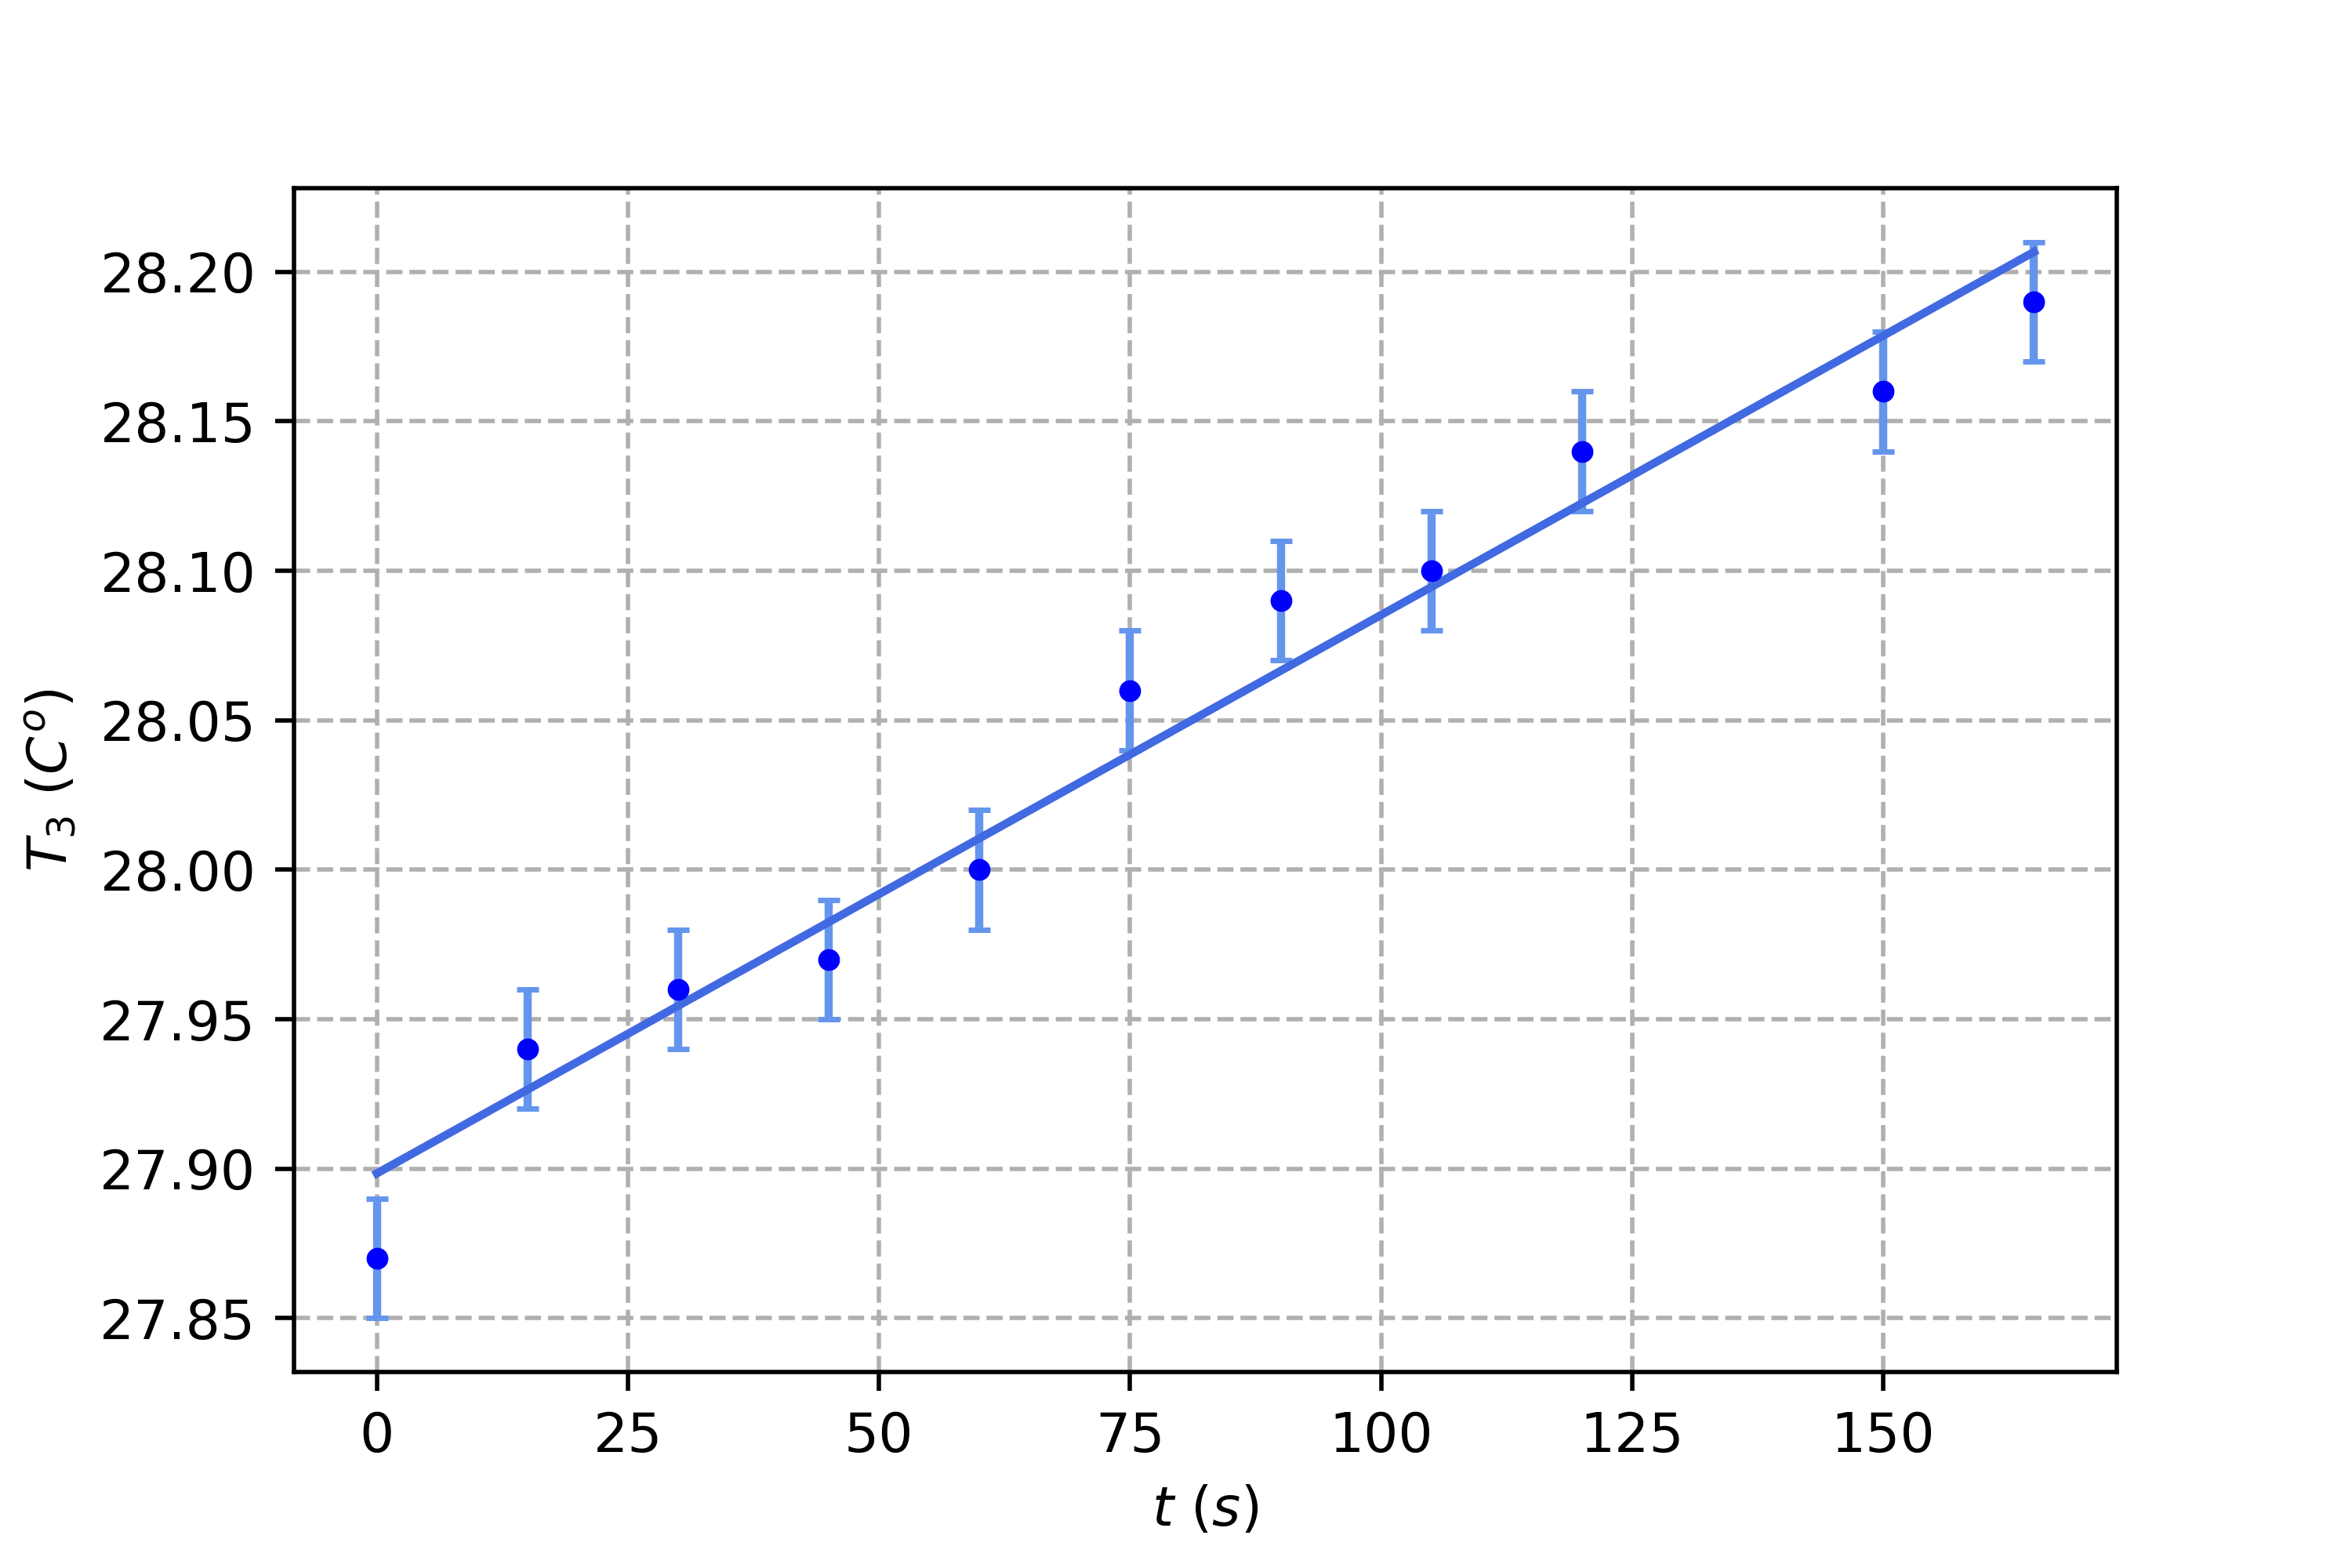
\includegraphics[scale=1.0]{plotT38.png} 
\caption{representación de $T_3$ frente a $t$ para $Q = 1.167 \ g/s$ e $d = 50$ cm} 
\label{Fig:plot-9}  
\end{figure} 
 
\newpage 
 
 
 
 
\subsubsection{Caudal número 5} 
 
Usando los datos del apartado \ref{subsec:10} y los  resultados experimentales de la regreisón lineal (tab \ref{tab:regresion10}) (fig \ref{Fig:plot-10}), podemos calcular las energías 
 
 \begin{equation} 
\begin{array}{lllllll}
E_1 & = & 146.6 W &  \ \ &  s(E_1) & =  & 8.9  W \\ 
 E_2 & = & 47.8 W &  \ \ &  s(E_2) & =  & 1.9  W \\ 
 E_3 & = & 28.5 W &  \ \ &  s(E_3) & =  & 3.1  W \\ 
 \end{array} 
\end{equation} 
 
 y podemos calcular los rendimientos 
 
\begin{equation} 
\begin{array}{lllllll}
\eta_1 & = & 0.326  &  \ \ &  s(\eta_1) & =  & 0.024   \\ 
 \eta_2 & = & 0.597  &  \ \ &  s(\eta_2) & =  & 0.069   \\ 
 \eta_3 & = & 0.195  &  \ \ &  s(\eta_3) & =  & 0.024   \\ 
 \end{array} 
\end{equation} 
 
 \begin{table}[h!] 	 \centering 
\begin{tabular}{|c|c|c|c|} 
\hline 
$a \ (C^o)$ & $s(a) \ (C^o)$ & $ b \ (C^o/s)$ & $s(b) \ (C^o/s)$  \\ \hline 
29.172  & 0.010 &  0.00092 & 0.00010\\ 
\hline
\end{tabular} 
\caption{Valores del ajuste lineal para los pares ($t,T_3$) con $Q=0.733 \ (g/s)$ y $d= 50 $ cm} 
\label{tab:regresion10} 
\end{table} 
 
 
\begin{figure}[h!] 	 \centering 
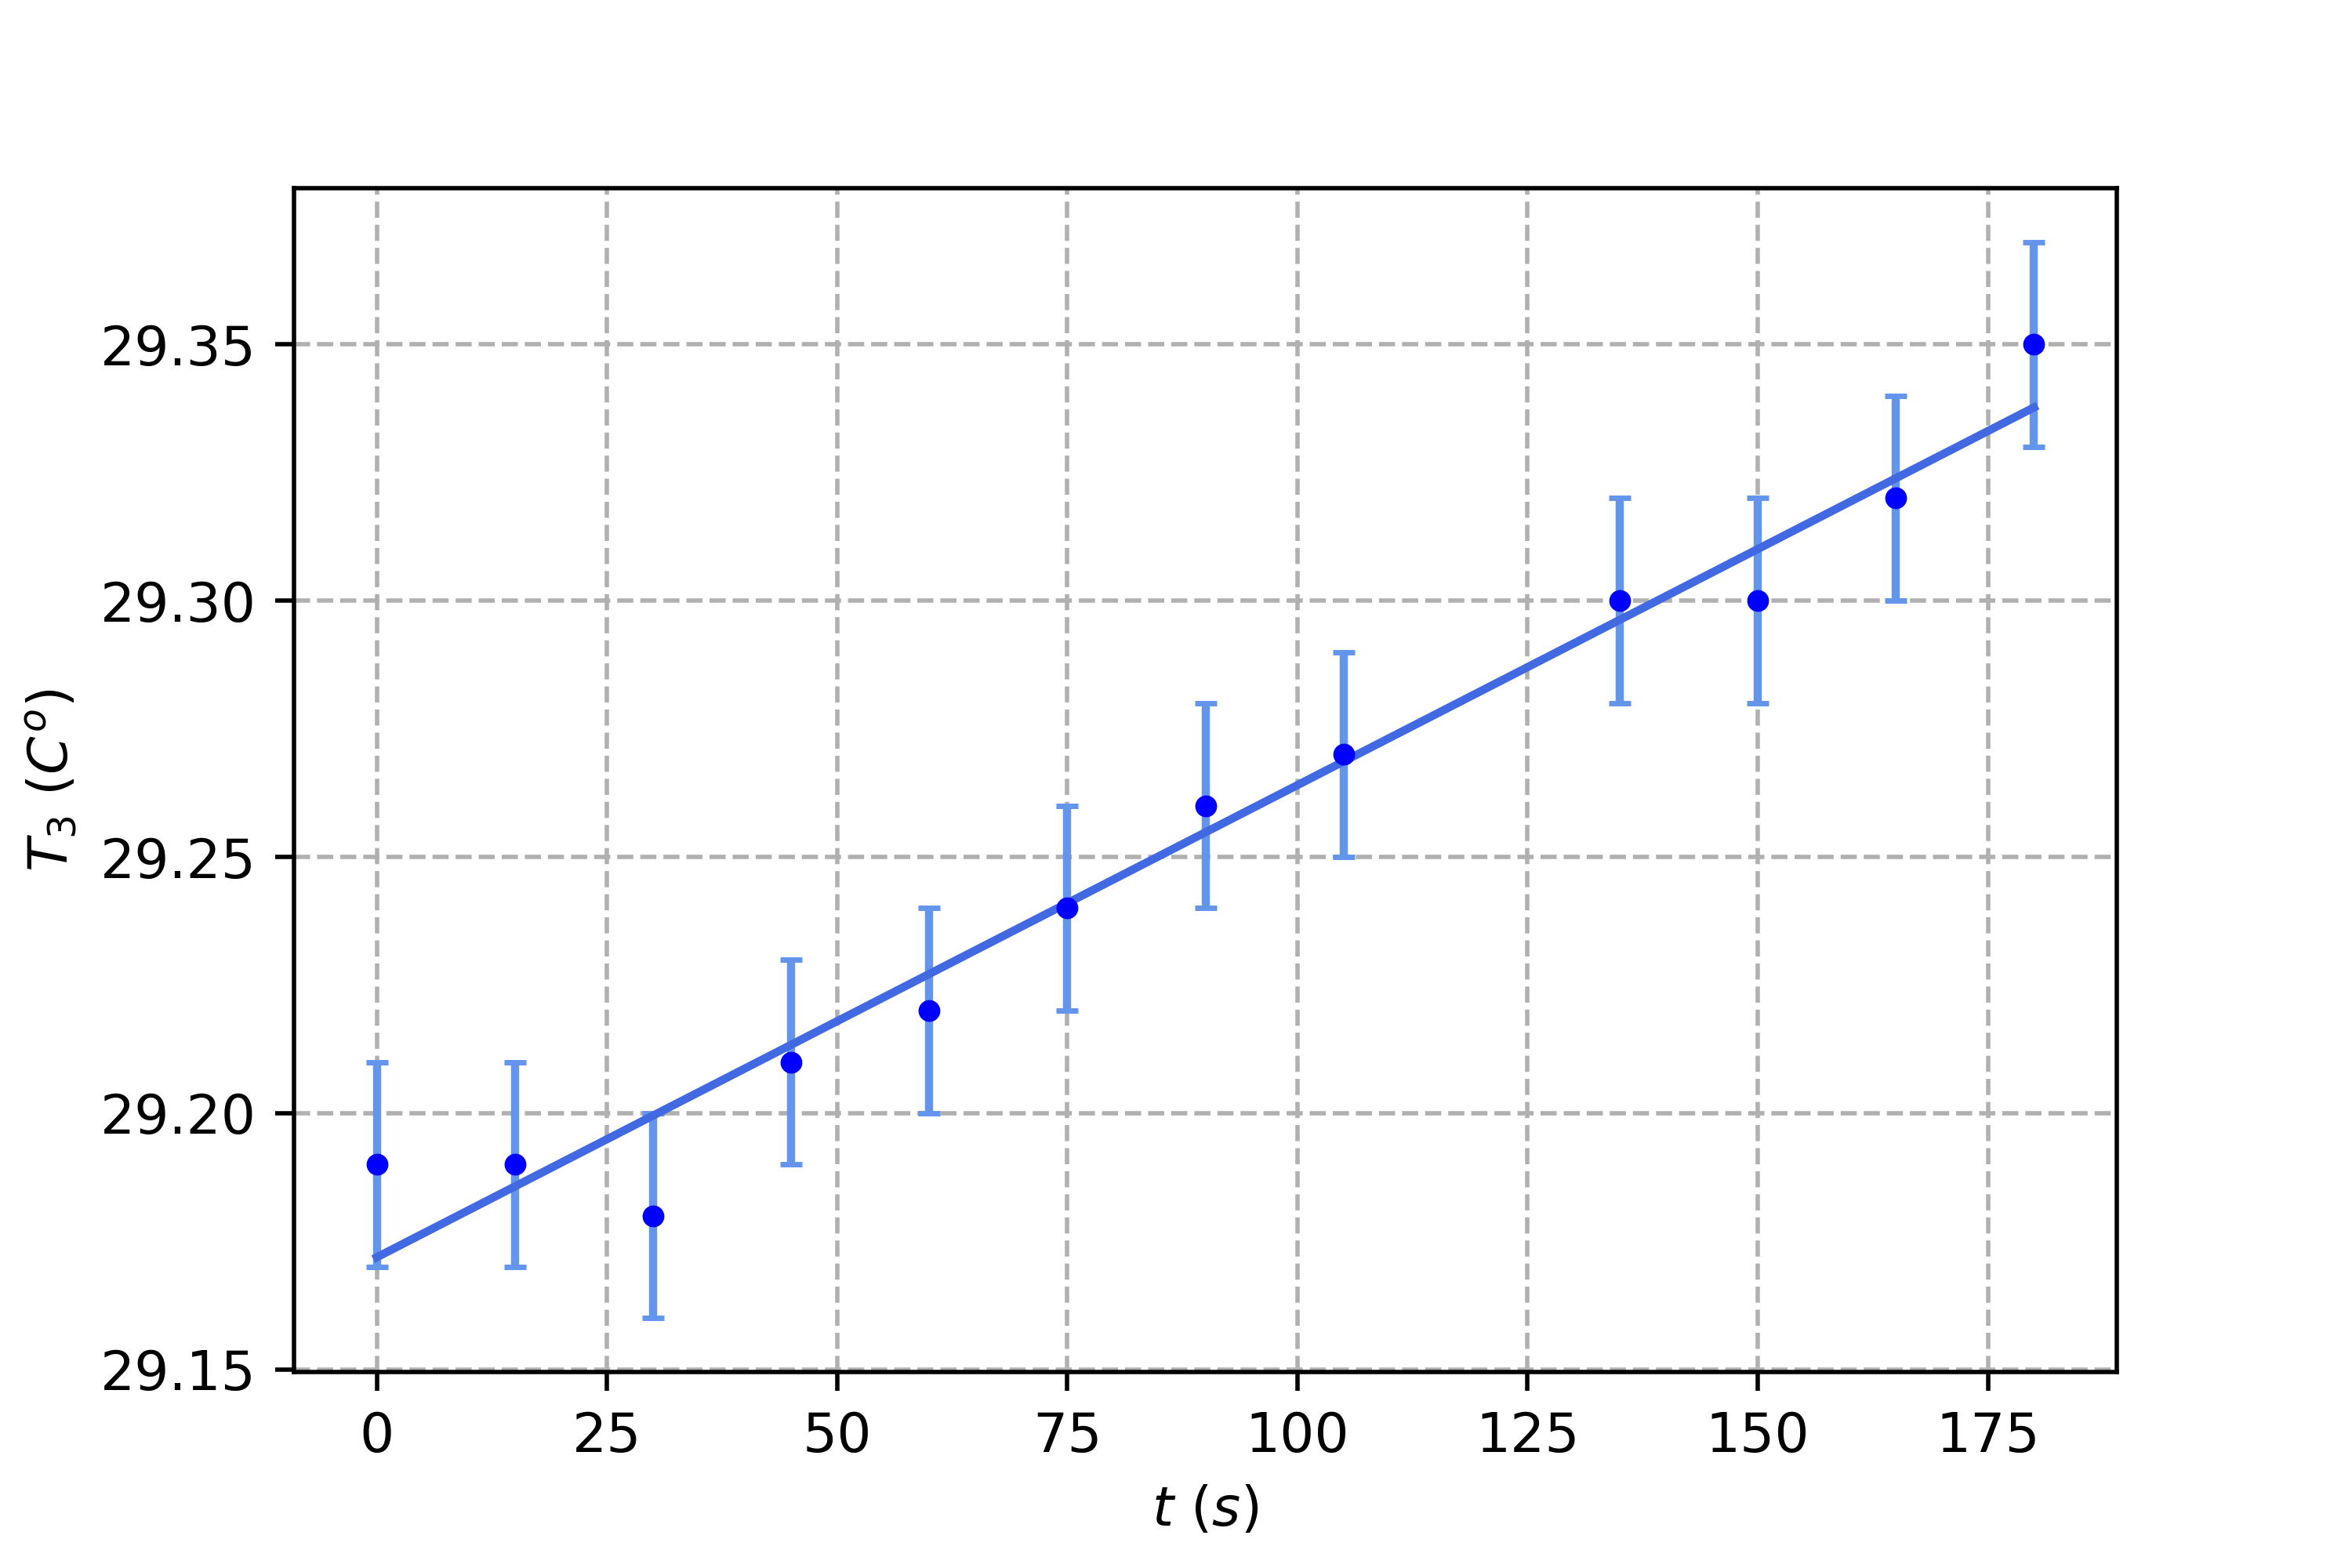
\includegraphics[scale=1.0]{plotT39.png} 
\caption{representación de $T_3$ frente a $t$ para $Q = 0.733 \ g/s$ e $d = 50$ cm} 
\label{Fig:plot-10}  
\end{figure} 
 
\newpage 
 
 
 
 
 
\newpage 
 
\subsection{Gráficas} \label{subsec:graficas}

En este apartado se representarán algunas gráficas que serán un desarrollo de los resultados obtenidos, basándonos en ellos, pero aportando una información más directa y visual. Aquí solo las representaremos y las comentaremos muy brevemente: el análisis mas detallado se realizará en la sección de conclusiones.  \\

En las figuras \ref{Fig:plot-11} y \ref{Fig:plot-12} estamos comparando los rendimientos en función del caudal para una distancia concreta. \\


En las figuras \ref{Fig:plot-13} y \ref{Fig:plot-14} representamos las  energías $E_2$ y $E_3$ respecto al caudal distinguiendo la distancia en función del color de los puntos. En este caso representamos esto para dar una mejor perspectiva de como se comportan las energías, ya que aunquue los rendimientos de una distancia sean mayores o menores que los que otro, no implica que las energías lo sean. Puede que el cociente sea menor pero no sus  energías, como es el caso. \\


En la figura \ref{Fig:plot-15} representé de manera mas concreta los rendimientos $eta_3$ para cada distancia y caudal. Es preciso realizar una gráfica así, ya que al final toda la práctica se basa en estudiar el rendimiento de la placa solar que calienta el depósito, y lo que nos da dicho valor no es más que $\eta_3$. 


\begin{figure}[h!] 	 \centering 
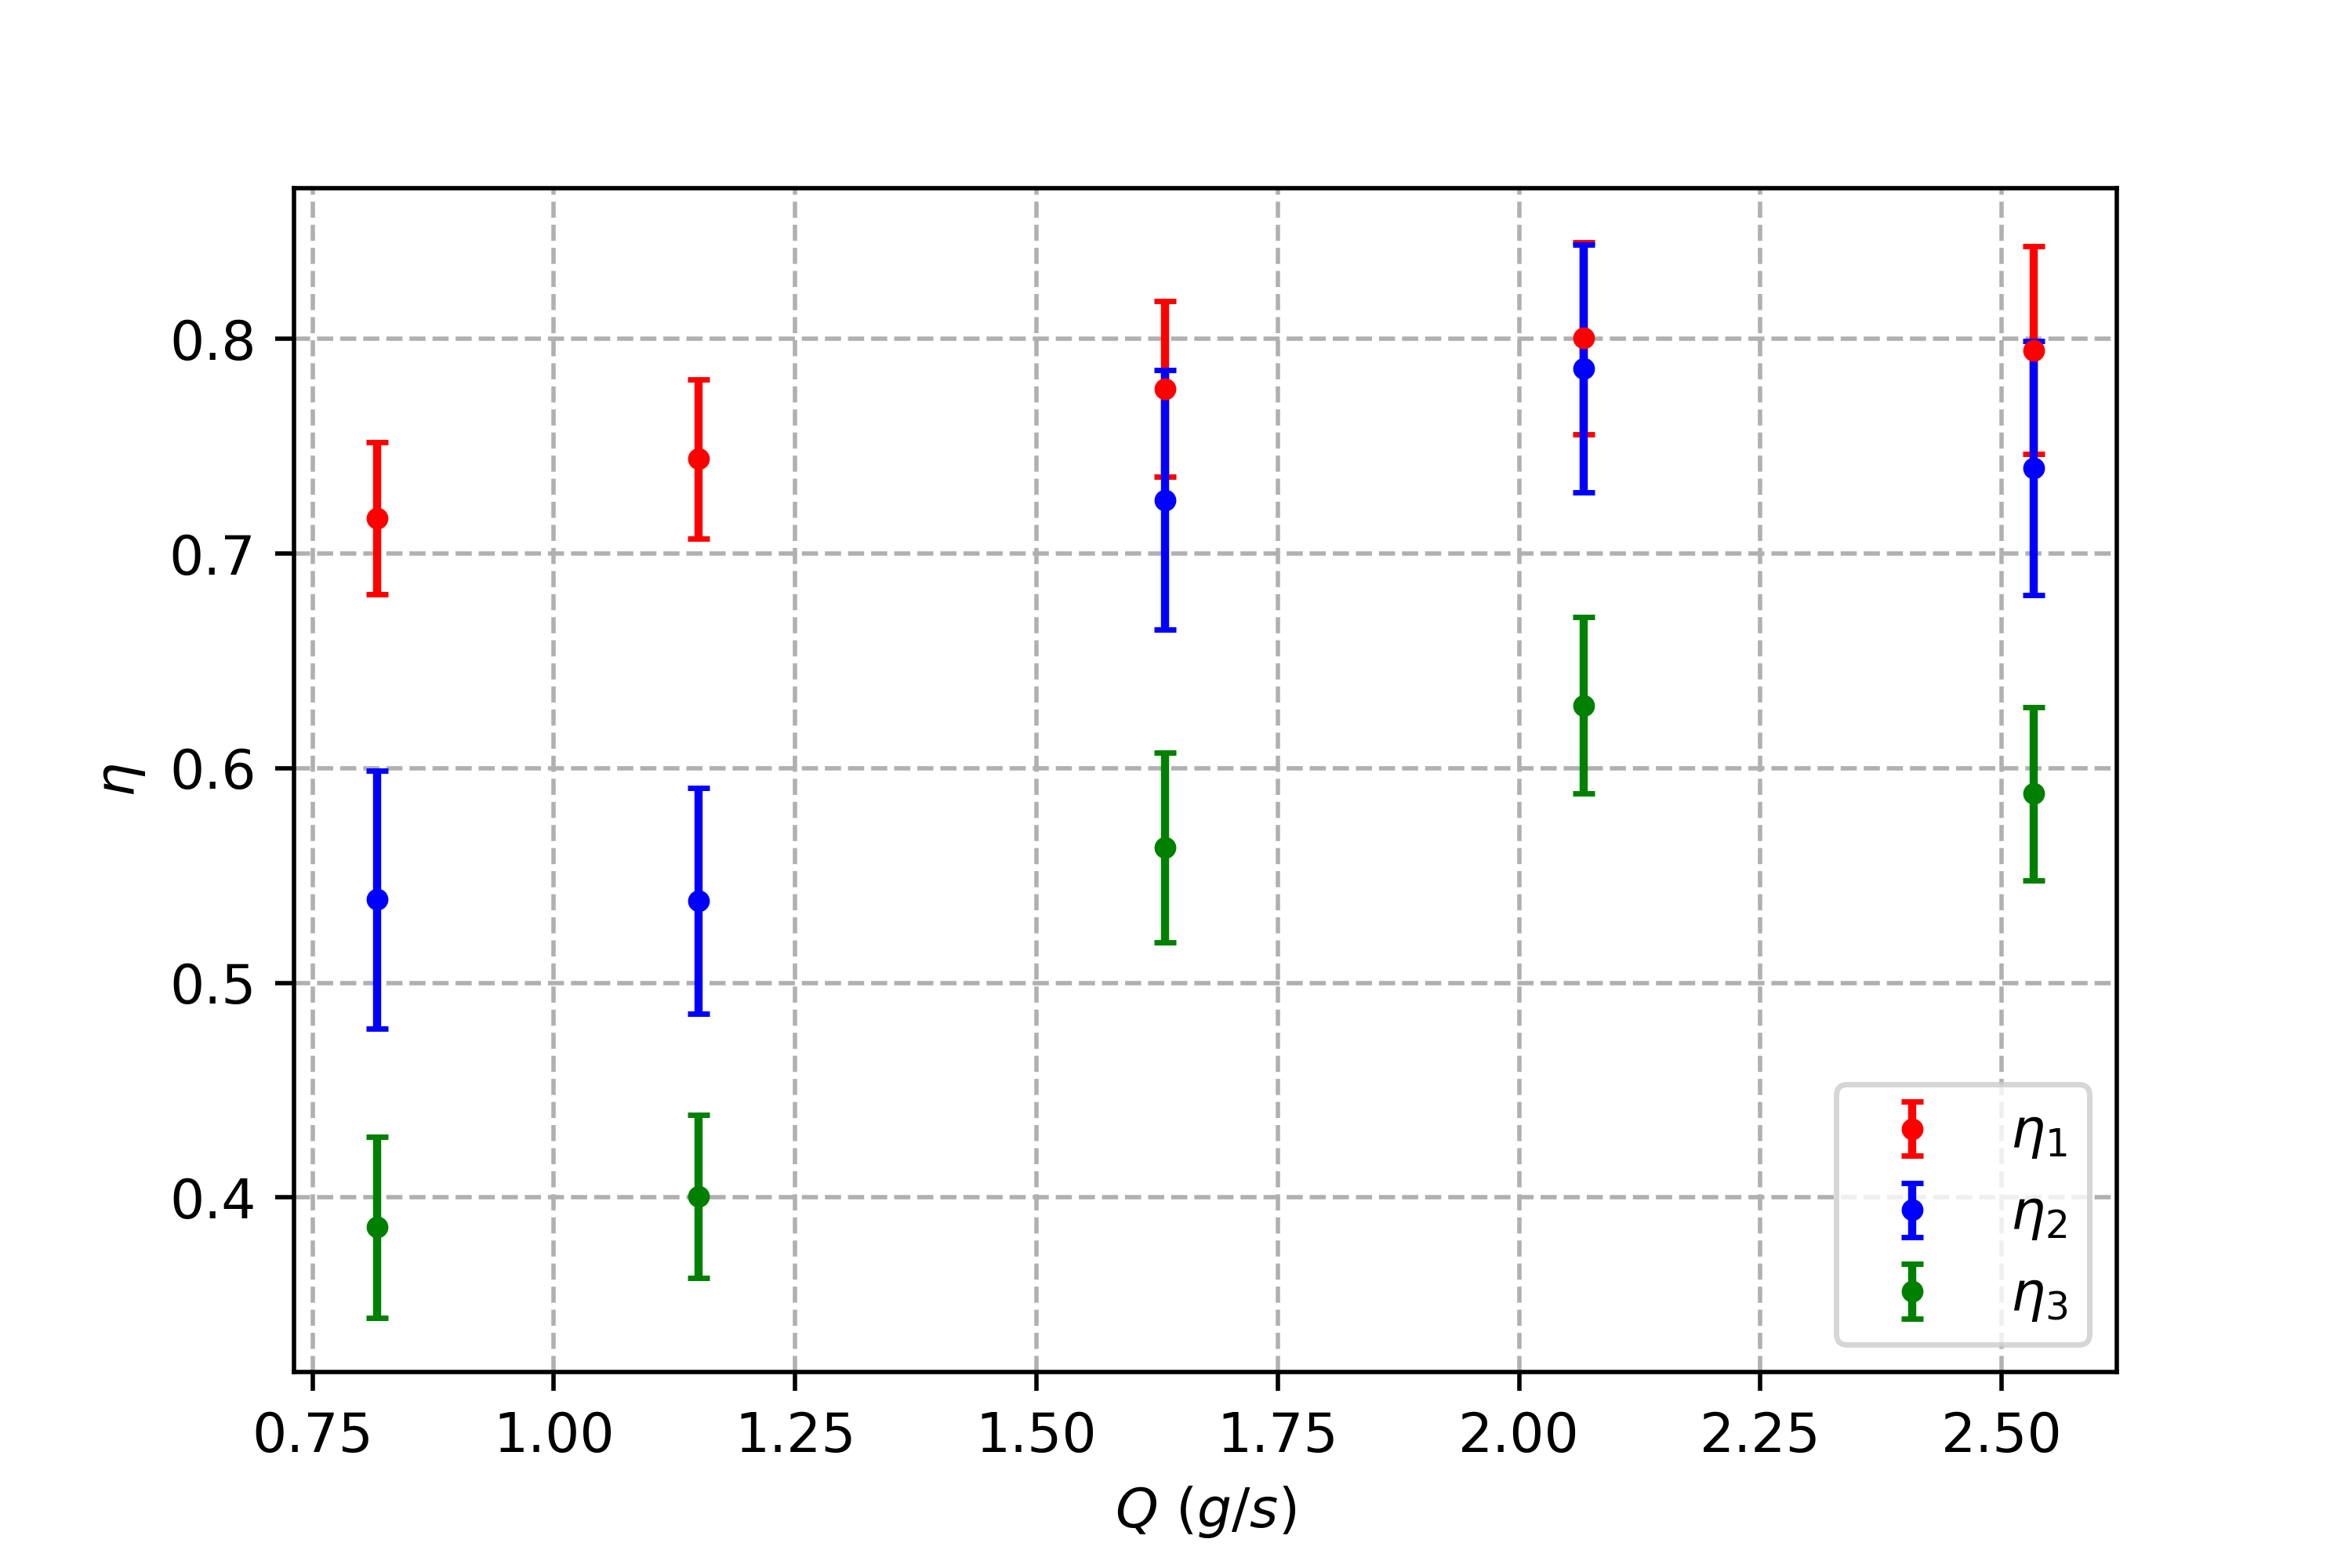
\includegraphics[scale=1]{etad1.png} 
\caption{representación de $\eta$ frente a $Q$ para  $d = 75$ cm} 
\label{Fig:plot-11}  
\end{figure} 

\newpage

\begin{figure}[h!] 	 \centering 
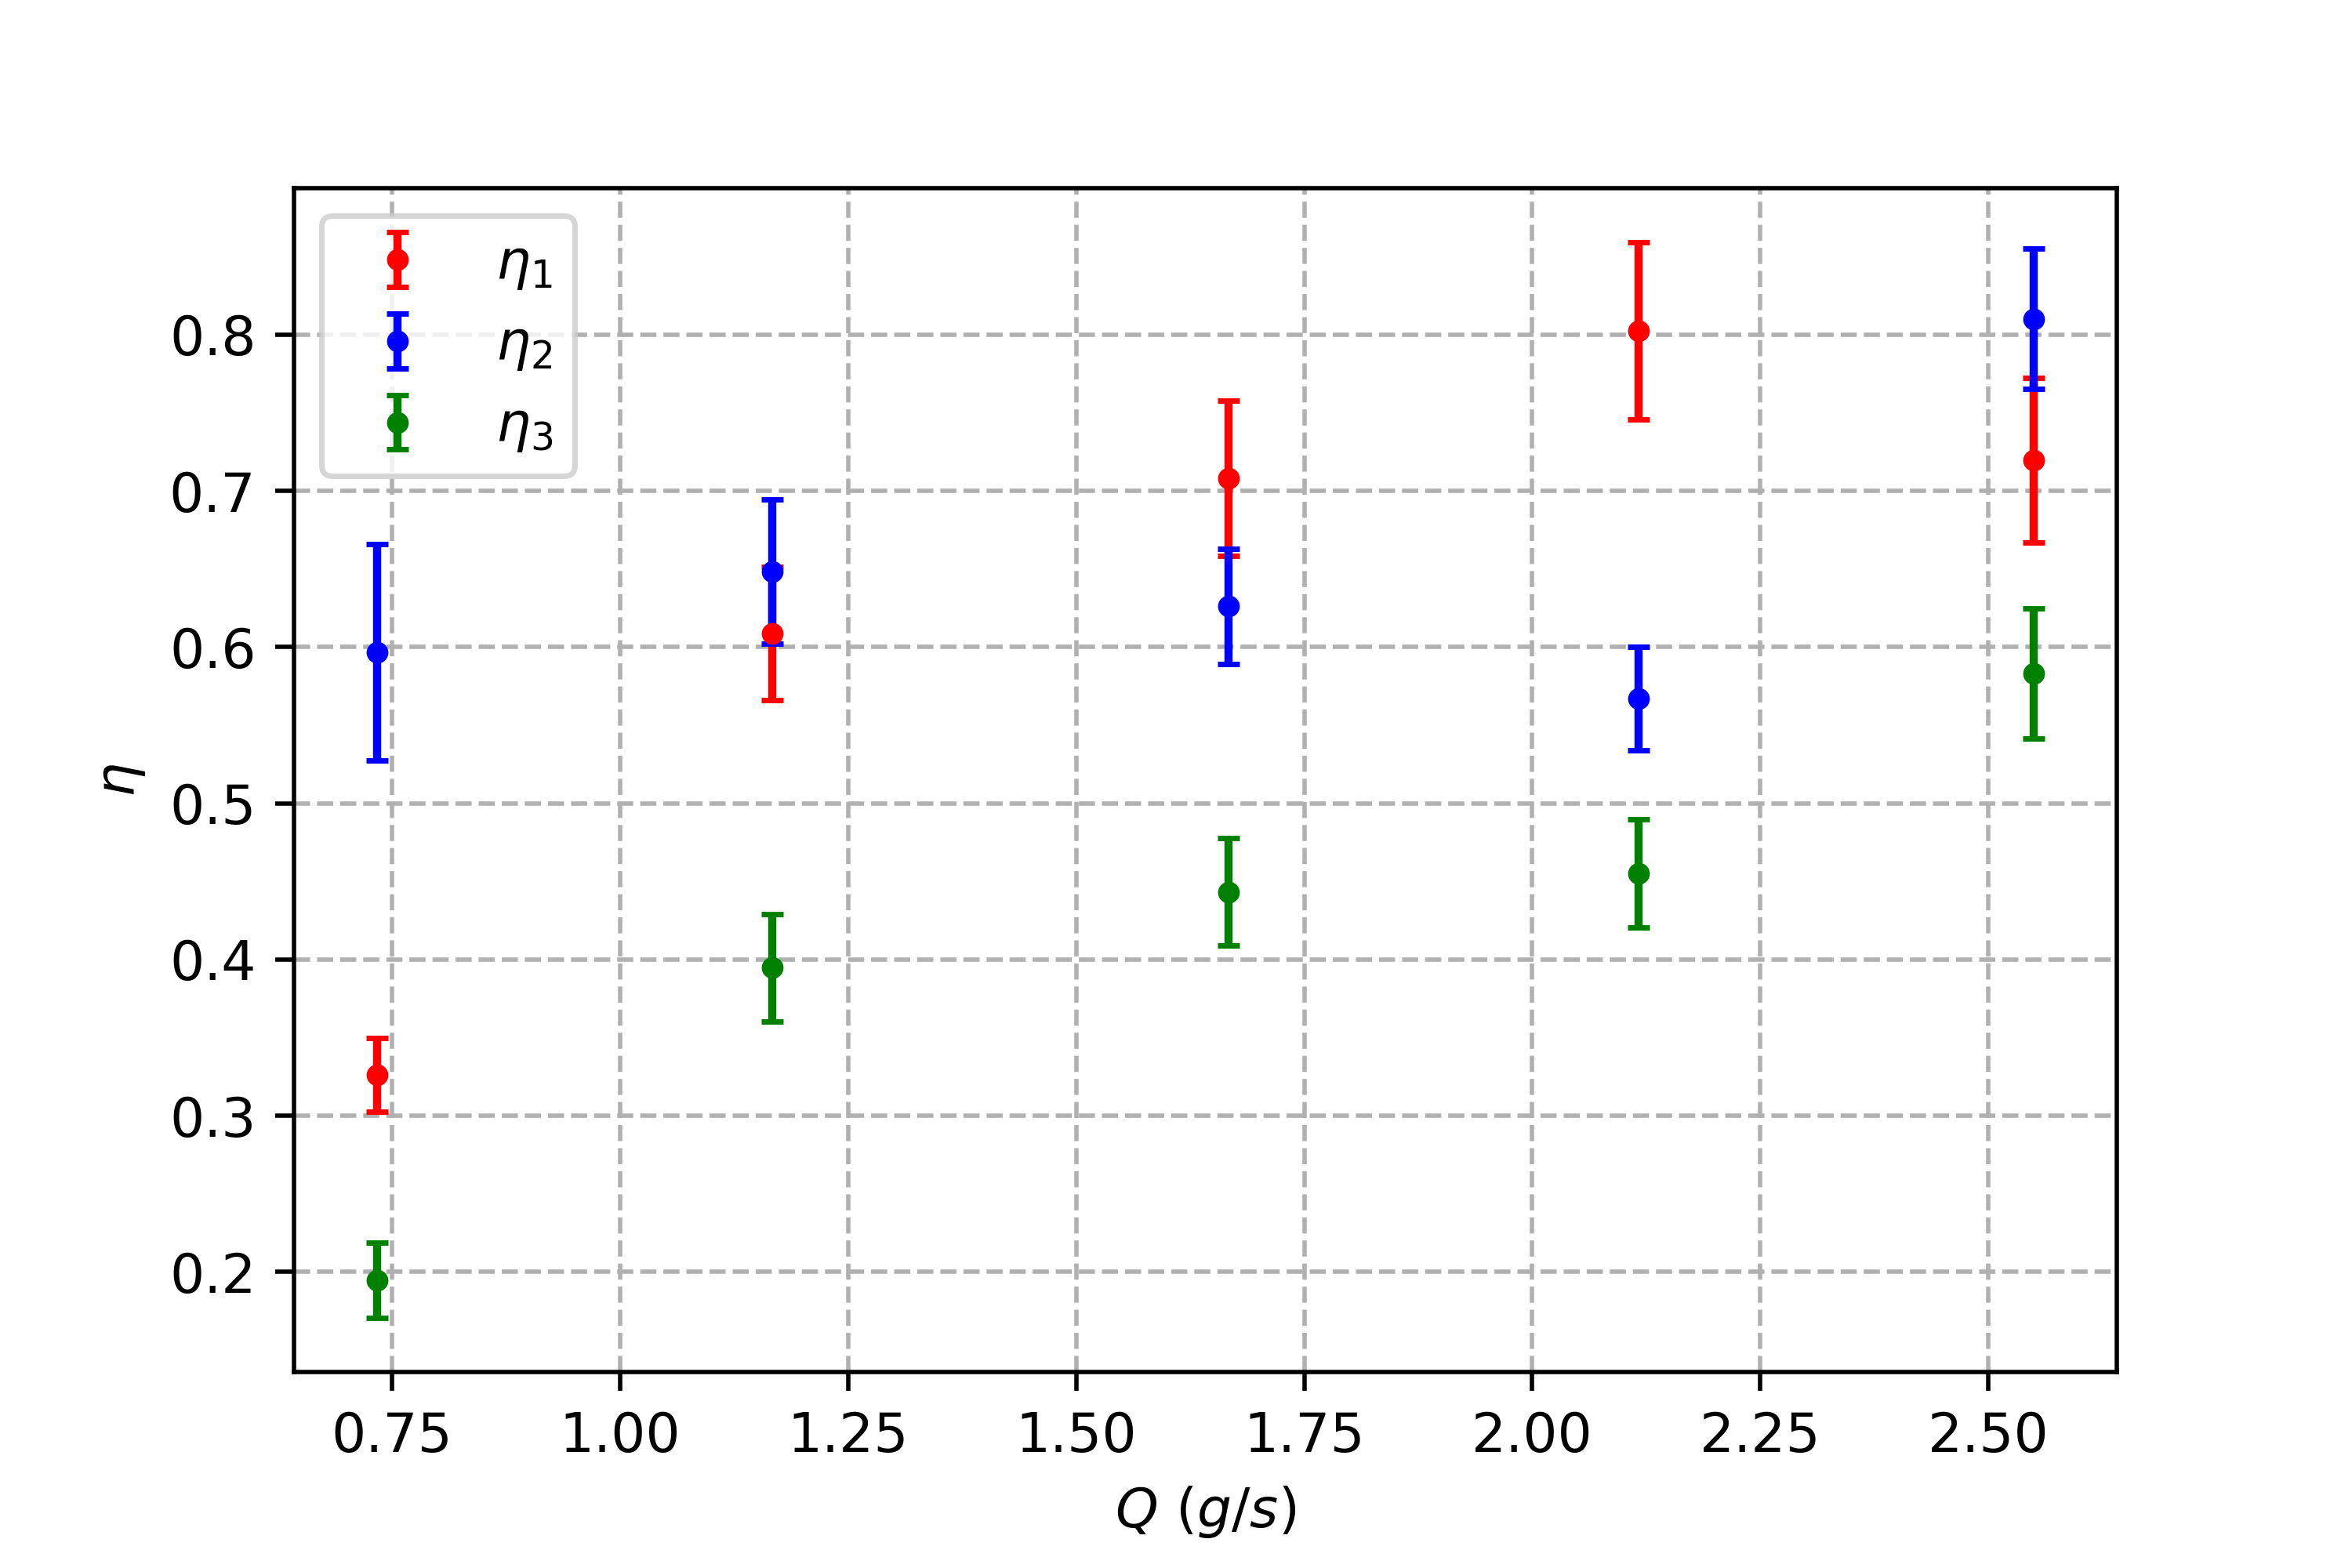
\includegraphics[scale=1]{etad2.png} 
\caption{representación de $\eta$ frente a $Q$ para  $d = 50$ cm} 
\label{Fig:plot-12}  
\end{figure} 

\begin{figure}[h!] 	 \centering 
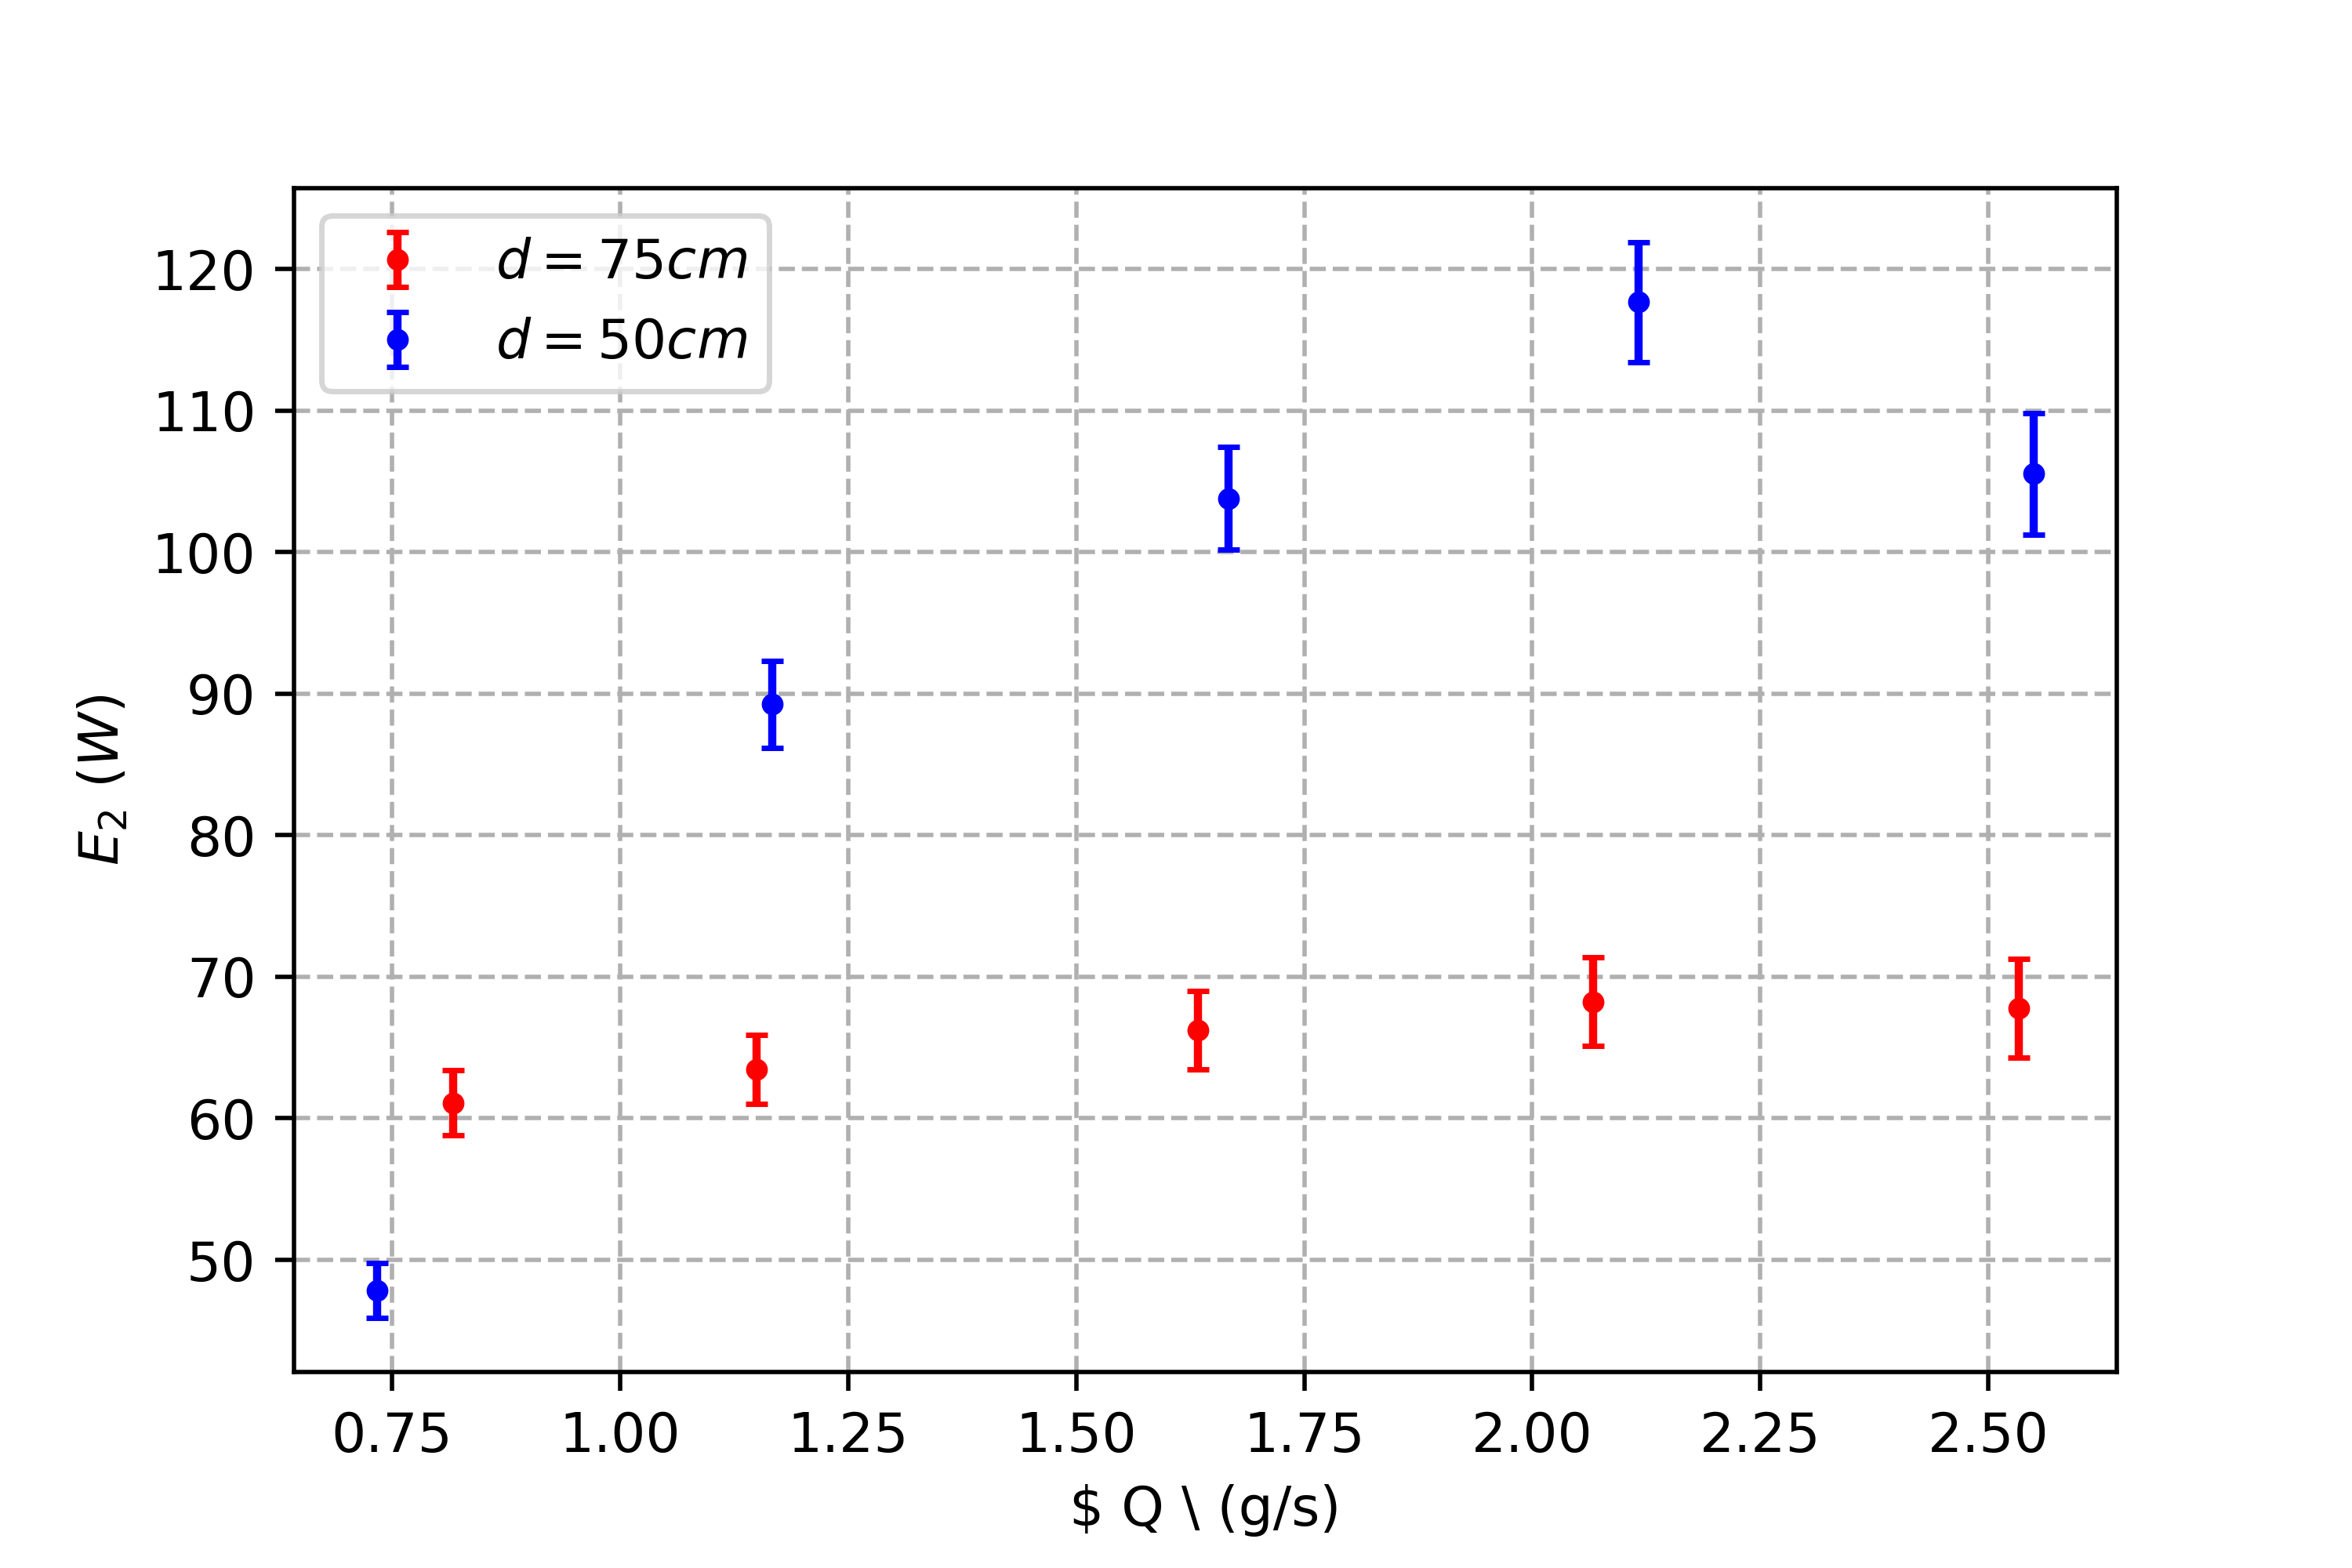
\includegraphics[scale=1]{E2-comparacion.png} 
\caption{representación de $E_2$ frente a $Q$ para las dos distancias} 
\label{Fig:plot-13}  
\end{figure} 

\newpage

\begin{figure}[h!] 	 \centering 
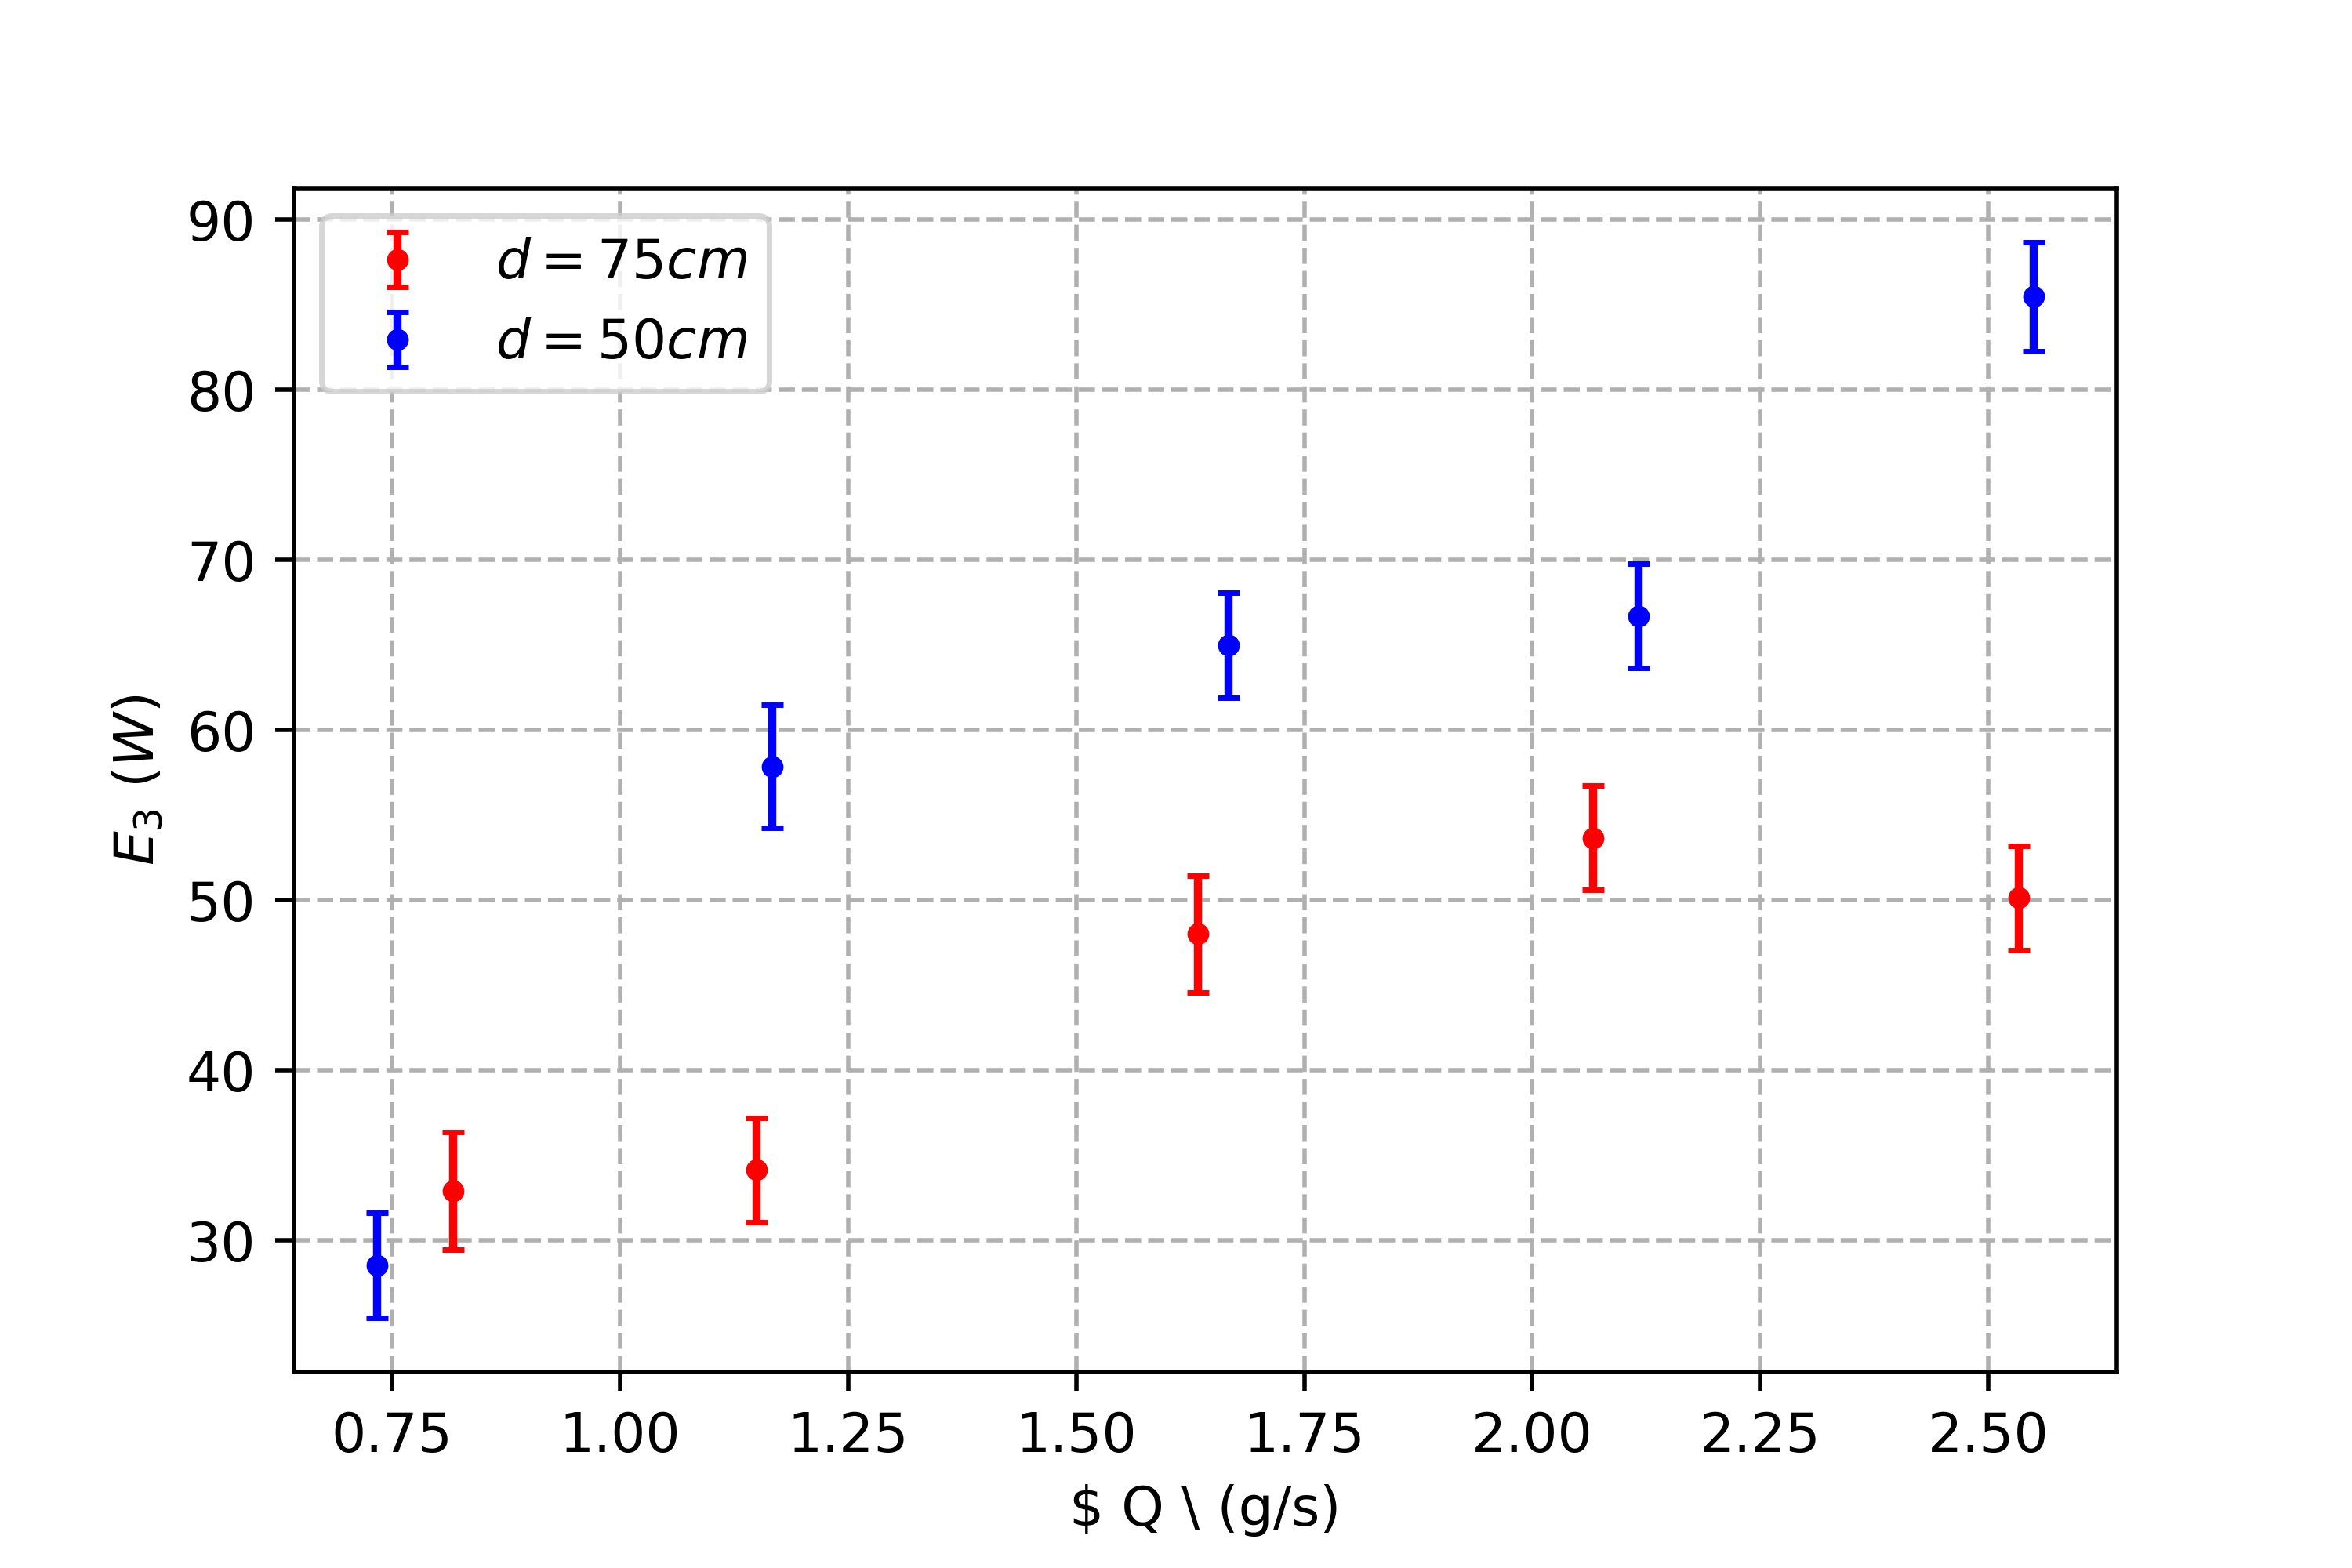
\includegraphics[scale=1]{E3-comparacion.png} 
\caption{representación de $\eta$ frente a $Q$ para para las dos distancias} 
\label{Fig:plot-14}  
\end{figure} 

\begin{figure}[h!] 	 \centering 
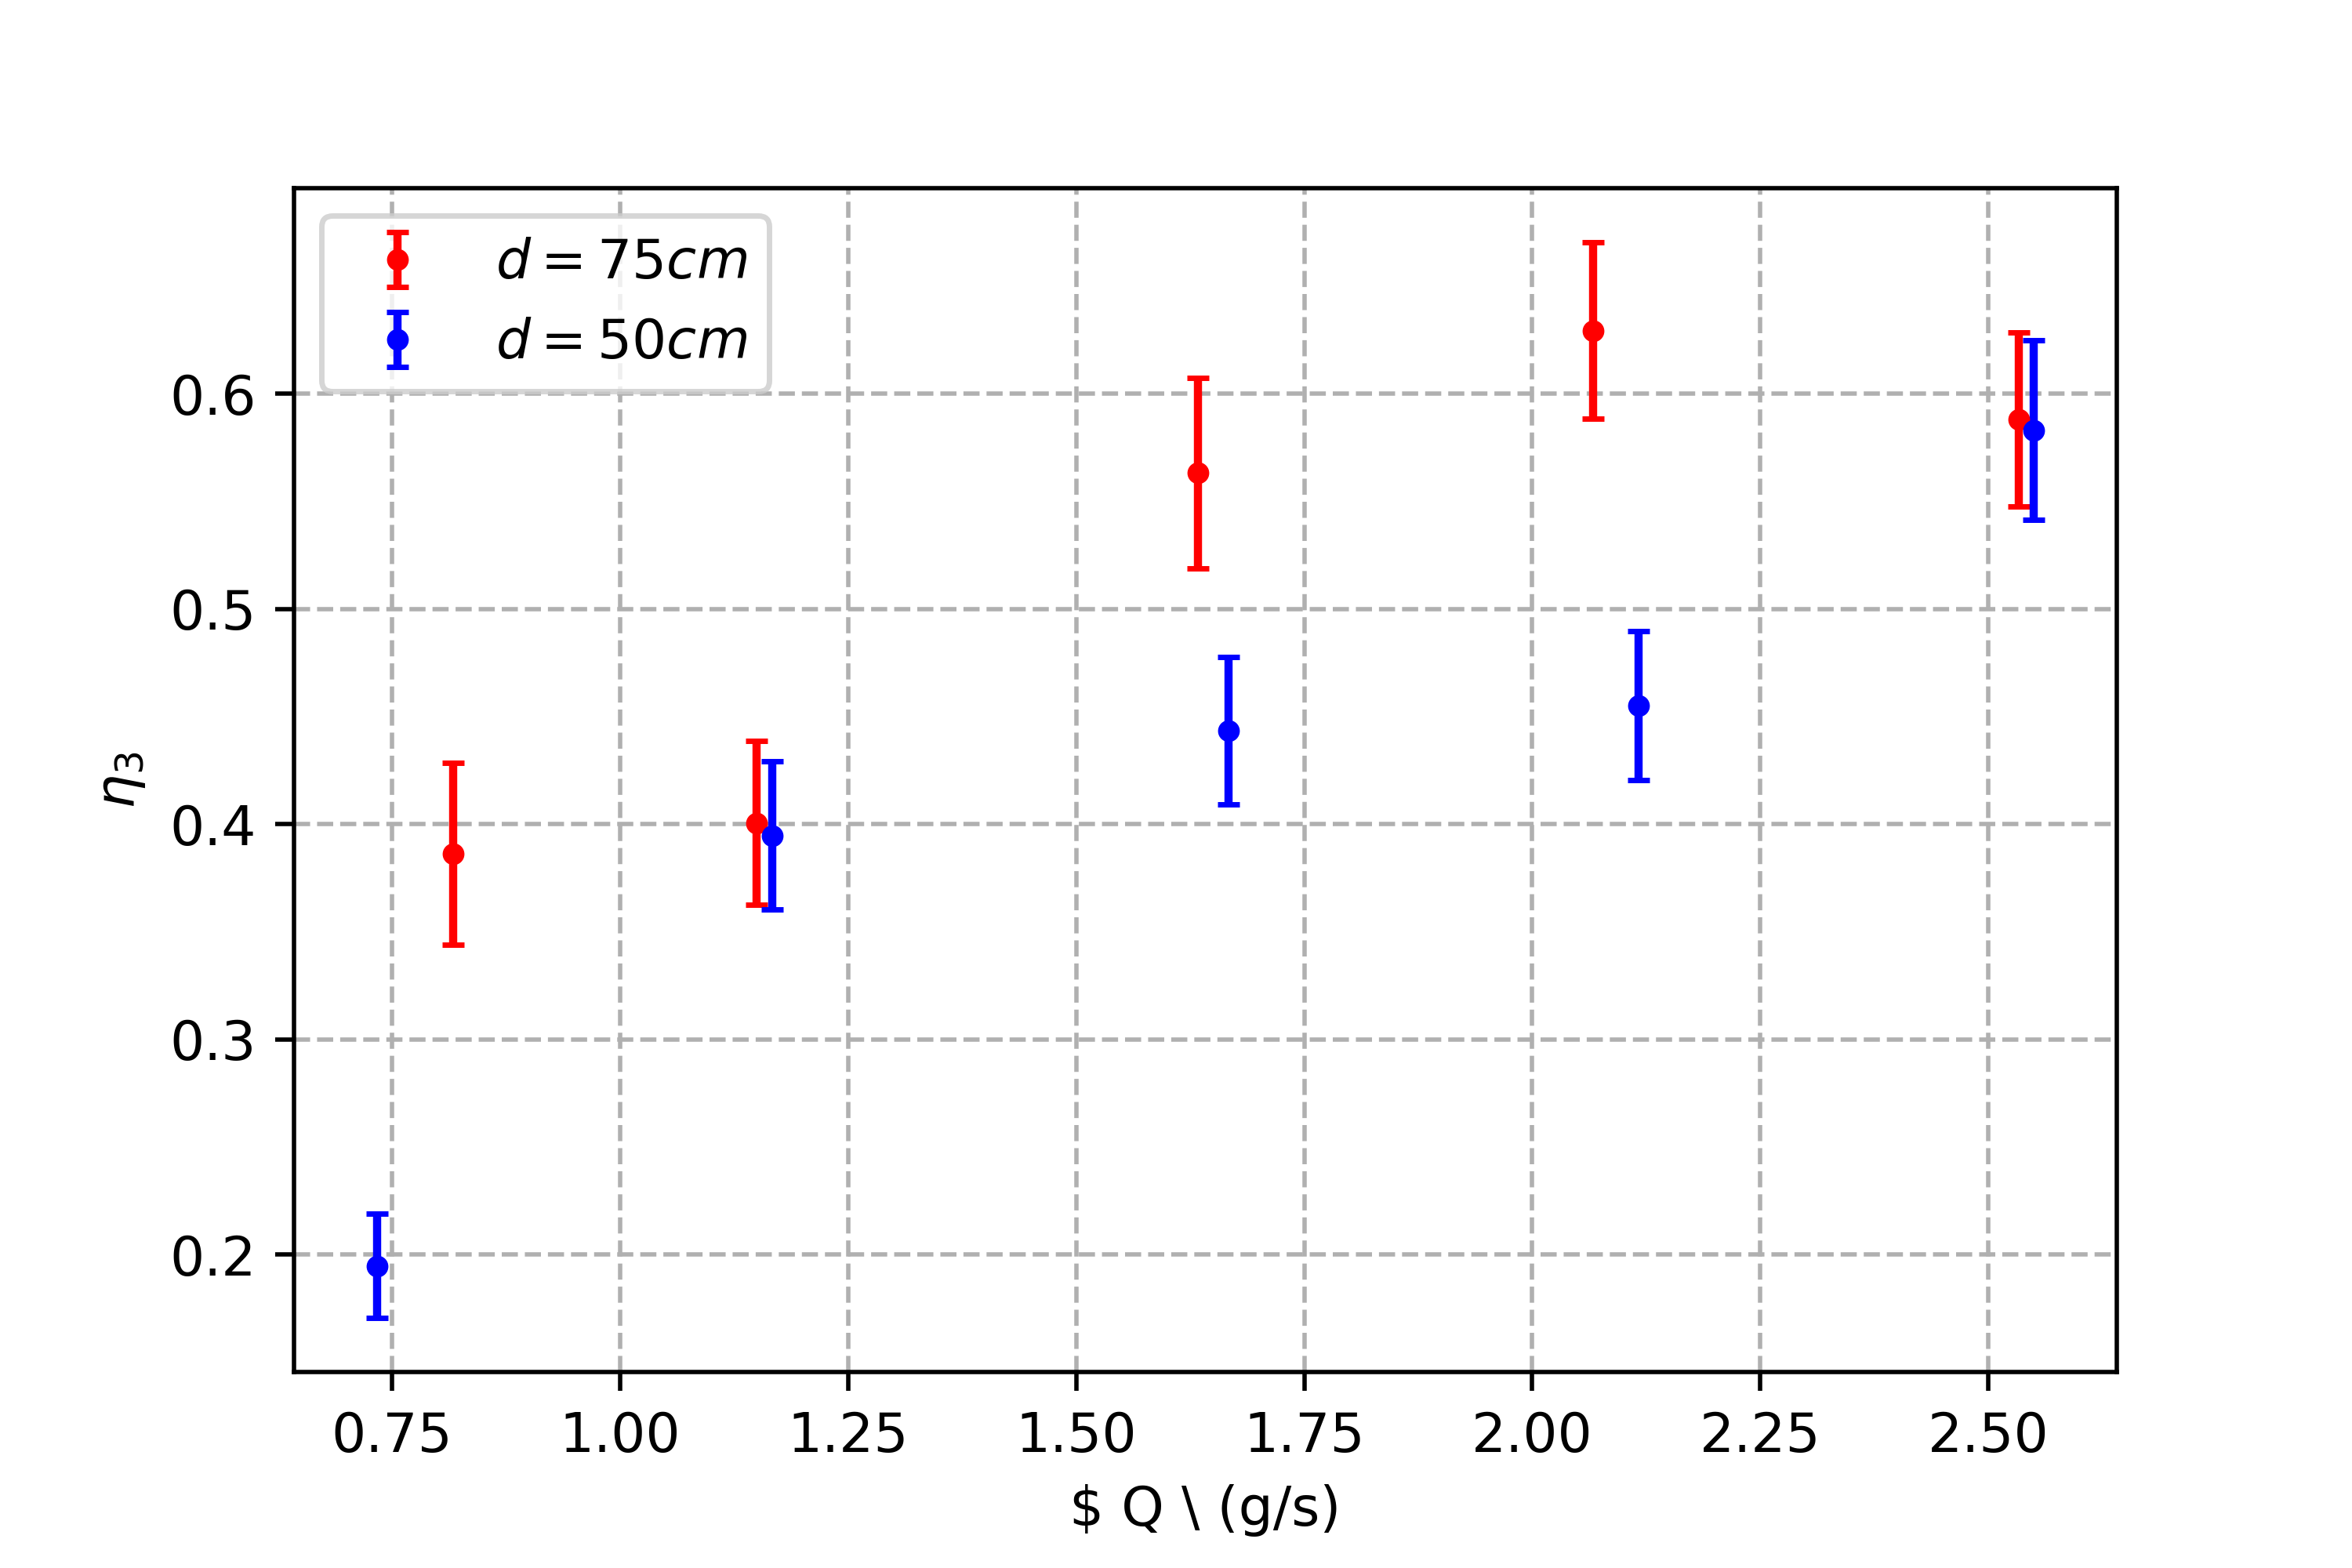
\includegraphics[scale=1]{eta3-comparacion.png} 
\caption{representación de $\eta$ frente a $Q$ para las dos distancias} 
\label{Fig:plot-15}  
\end{figure} 

\newpage

\section{Conclusión}

En esta sección vamos a tratar todo lo referente al análisis de los resultados. \\

Nuestro principal objetivo en la práctica era calcular el rendimiento de la placa solar, por lo que primero analizaremos un poco la calidad de los resultados: que afecta a la toma de datos, que se puede incluir para reducir la incertidumbre... para estudiar si los resultados se pueden considerar exitosos o no. Luego analizaremos el otro objetivo de la práctica, que es estudiar el rendimiento de la placa solar en función del caudal y la distancia placa-foco. En esta parte nos apoyaremos en las gráficas del apartado \ref{subsec:graficas} para entenderlo un poco mejor. \\

Para estudiar si nuestros resultados han sido o no satisfactorios nos basaremos en los siguientes puntos: ¿Hemos considerado la mayor parte de los focos de incertidumbre, o por el contrario existen parámetros que de tenerlos en cuenta cambiarían toda la práctica?¿El resultado obtenido era lo que cabría esperar?. \\

En general considero bastante satisfactoria la toma de los datos en nuestra práctica. Tanto el caudal, como la $\Delta T$ fue tomada con una precisión bastante buena, y aunque alguna vez oscilase, simplemente le asignamos un valor a la incertidumbre mas grande. En la toma de datos de los pares de valores ($t,T_3$) si que hemos tenido al o mejor un poco mas de desajuste, y una oscilación mucho mayor. Yo considero que se debe un poco a que la precisión del termómetro digital es muy elevada (0.01 $C^o$), y con esa precisión un mínimo cambio en la temperatura afecta mucho. Además la propagación de la temperatura del depósito no es homogéneo, y existen puntos mas calientes que otros por lo que aparecerán corrientes de agua que producen dicha oscilación. De todos modos esta parte de la incertidumbre la hemos incluido al considerar toda posible naturaleza de la oscilación. A pesar de esto, las regresiones lineales son bastante buenas, y si ve claramente el comportamiento lineal. \\

Sin embargo si que existe un foco de incertidumbre, no muy elevada, pero que no hemos incluido. Estás son la incertidumbre de la capacidad calorífica y la incertidumbre del pinanómetro de Zipp-Komen. Aunque en general la capacidad calorífica es constante a 1 atm; en realidad varía con la temperatura, algo que no hemos tenido en cuenta, ni siquiera le hemos dado una incertidumbre, lo hemos considerado un valor tabulado. Lo mismo para la expresión de la intensidad en función de la distancia. De todos modos esto no afectará mucho a la práctica. Obviamente tener en cuenta está información hará que la práctica sea mas rigurosa, pero para nuestro nivel, los focos de incertidumbre contempladas serán suficiente. \\

Además los resultados finales son muy buenos: no nos da un rendimiento mayor que uno (por lo que no viola el segundo principio de la termondinámica), pero tampoco nos da un rendimiento muy pequeño. Esto es lo que cabría esperar: ya sabíamos que no toda la energía que entra por la placa puede convertirse en calor, siempre hay perdidas. Por todo lo dicho anteriormente podemos considerar la práctica un éxito. \\

Ahora vamos a analizar un poco las figuras. Como podemos ver en la figura \ref{Fig:plot-13} la energía que pasa de la placa al circuito aumenta con el caudal, así como que aumenta al disminuir la distancia. Esto responde a lo que podríamos esperar: cuanto mas cerca este la placa del foco mas energía va absorber y más podrá captar el circuito. Aunque existan pequeñas anomalías, en general el comportamiento es el dicho. De hecho podemos ver que para la distancia de d=50cm el comportamiento es mucho menos estable, lo que implica que a grandes temperaturas (del agua del circuito) se comporta de manera mas errática. También vemos que a caudales muy pequeños disminuye mucho la energía que se trasmite, de manera muy pronunciada. Esto también se ve representado en la figura \ref{Fig:plot-14}. 

Mientras que se ve claramente que las energías son mayores para la distancia, el rendimiento es menor para la distancia menor. Esto es, probablemente, porque no es captar de igual manera toda la energía que llega, por lo que el rendimiento es menor. Es comprensible que sea menor, de hecho, es lo que cabe esperar. De todos modos podemos ver que, excepto por un valor, a menor caudal menor rendimiento. \\

En conclusión, podemos decir que está práctica a dado unos resultados que podríamos esperar, y aunque es mejorable, estudia el rendimiento de los dos factores que mas influyen en la placa solar: la distancia foco-placa y caudal. Quizás hacer un par mas de distancias y mas caudales daría mas información. 



\newpage


\section{Datos}  \label{Sec:datos}
\subsection{Primera distancia}
 
La primera distancia que tomamos fue: 
 
\begin{equation} 
\begin{array}{lllllll}
d & = & 6.40 m &  \ \ &  s(d) & =  & 0.33  m \\ 
 I & = & 763 W/m^2 &  \ \ &  s(I) & =  & 23 W/m^2 \\ 
 S & = & 0.112 m^2 &  \ \ &  s(S) & =  & 0.001  m^2 \\ 
 \end{array} 
\end{equation} 
 
 \subsubsection{Caudal número 1} \label{subsec:1} 
 
Podemos ver el caudal e intensidad en la siguiente ecuación y los pares de valores ($t,T_3$) en la tabla \ref{tab:datoscrudos0}: 
 
\begin{equation} 
\begin{array}{lllllll}
\Delta T & = & 6.40 C^o &  \ \ &  s(\Delta T) & =  & 0.33  C^o \\ 
 Q & = & 2.533 g/s &  \ \ &  s(Q) & =  & 0.017  g/s \\ 
 \end{array} 
\end{equation} 
 
 \begin{table}[h!] 	 \centering 
\begin{tabular}{|c|c|c|c|} 
\hline 
$T_3 \ (C^o)$ & $s(T_3) \ (C^o)$ & $ t \ (s)$ & $s(t) \ (s)$  \\ \hline 
19.06  & 0.02 &  15 & 1 \\ 
\hline
19.09  & 0.02 &  30 & 1 \\ 
\hline
19.12  & 0.02 &  45 & 1 \\ 
\hline
19.14  & 0.02 &  60 & 1 \\ 
\hline
19.16  & 0.02 &  75 & 1 \\ 
\hline
19.18  & 0.02 &  90 & 1 \\ 
\hline
19.21  & 0.02 &  105 & 1 \\ 
\hline
19.20  & 0.02 &  120 & 1 \\ 
\hline
19.22  & 0.02 &  135 & 1 \\ 
\hline
19.27  & 0.02 &  150 & 1 \\ 
\hline
19.30  & 0.02 &  165 & 1 \\ 
\hline
19.34  & 0.02 &  180 & 1 \\ 
\hline
19.38  & 0.02 &  195 & 1 \\ 
\hline
\end{tabular} 
\caption{Valores del ajuste lineal para los pares ($t,T_3$) con $Q=2.533 \ (g/s)$ y $d= 75 $ cm} 
\label{tab:datoscrudos0} 
\end{table} 
 
 \newpage
 
\subsubsection{Caudal número 2} \label{subsec:2} 
 
Podemos ver el caudal e intensidad en la siguiente ecuación y los pares de valores ($t,T_3$) en la tabla \ref{tab:datoscrudos1}: 
 
\begin{equation} 
\begin{array}{lllllll}
\Delta T & = & 7.90 C^o &  \ \ &  s(\Delta T) & =  & 0.36  C^o \\ 
 Q & = & 2.067 g/s &  \ \ &  s(Q) & =  & 0.017  g/s \\ 
 \end{array} 
\end{equation} 
 
 \begin{table}[h!] 	 \centering 
\begin{tabular}{|c|c|c|c|} 
\hline 
$T_3 \ (C^o)$ & $s(T_3) \ (C^o)$ & $ t \ (s)$ & $s(t) \ (s)$  \\ \hline 
20.66  & 0.02 &  15 & 1 \\ 
\hline
20.69  & 0.02 &  30 & 1 \\ 
\hline
20.71  & 0.02 &  45 & 1 \\ 
\hline
20.74  & 0.02 &  60 & 1 \\ 
\hline
20.76  & 0.02 &  75 & 1 \\ 
\hline
20.80  & 0.02 &  90 & 1 \\ 
\hline
20.83  & 0.02 &  105 & 1 \\ 
\hline
20.86  & 0.02 &  120 & 1 \\ 
\hline
20.87  & 0.02 &  135 & 1 \\ 
\hline
20.90  & 0.02 &  150 & 1 \\ 
\hline
20.93  & 0.02 &  165 & 1 \\ 
\hline
20.96  & 0.02 &  180 & 1 \\ 
\hline
20.95  & 0.02 &  195 & 1 \\ 
\hline
\end{tabular} 
\caption{Valores del ajuste lineal para los pares ($t,T_3$) con $Q=2.067 \ (g/s)$ y $d= 75 $ cm} 
\label{tab:datoscrudos1} 
\end{table} 
 
 \newpage
 
\subsubsection{Caudal número 3} \label{subsec:3} 
 
Podemos ver el caudal e intensidad en la siguiente ecuación y los pares de valores ($t,T_3$) en la tabla \ref{tab:datoscrudos2}: 
 
\begin{equation} 
\begin{array}{lllllll}
\Delta T & = & 9.70 C^o &  \ \ &  s(\Delta T) & =  & 0.39  C^o \\ 
 Q & = & 1.633 g/s &  \ \ &  s(Q) & =  & 0.017  g/s \\ 
 \end{array} 
\end{equation} 
 
 \begin{table}[h!] 	 \centering 
\begin{tabular}{|c|c|c|c|} 
\hline 
$T_3 \ (C^o)$ & $s(T_3) \ (C^o)$ & $ t \ (s)$ & $s(t) \ (s)$  \\ \hline 
22.41  & 0.02 &  0 & 1 \\ 
\hline
22.44  & 0.02 &  15 & 1 \\ 
\hline
22.47  & 0.02 &  30 & 1 \\ 
\hline
22.50  & 0.02 &  45 & 1 \\ 
\hline
22.51  & 0.02 &  60 & 1 \\ 
\hline
22.53  & 0.02 &  75 & 1 \\ 
\hline
22.56  & 0.02 &  90 & 1 \\ 
\hline
22.58  & 0.02 &  105 & 1 \\ 
\hline
22.60  & 0.02 &  120 & 1 \\ 
\hline
22.62  & 0.02 &  135 & 1 \\ 
\hline
22.65  & 0.02 &  150 & 1 \\ 
\hline
22.68  & 0.02 &  165 & 1 \\ 
\hline
\end{tabular} 
\caption{Valores del ajuste lineal para los pares ($t,T_3$) con $Q=1.633 \ (g/s)$ y $d= 75 $ cm} 
\label{tab:datoscrudos2} 
\end{table} 
 
\newpage 
 
\subsubsection{Caudal número 4} \label{subsec:4} 
 
Podemos ver el caudal e intensidad en la siguiente ecuación y los pares de valores ($t,T_3$) en la tabla \ref{tab:datoscrudos3}: 
 
\begin{equation} 
\begin{array}{lllllll}
\Delta T & = & 13.20 C^o &  \ \ &  s(\Delta T) & =  & 0.46  C^o \\ 
 Q & = & 1.150 g/s &  \ \ &  s(Q) & =  & 0.017  g/s \\ 
 \end{array} 
\end{equation} 
 
 \begin{table}[h!] 	 \centering 
\begin{tabular}{|c|c|c|c|} 
\hline 
$T_3 \ (C^o)$ & $s(T_3) \ (C^o)$ & $ t \ (s)$ & $s(t) \ (s)$  \\ \hline 
23.63  & 0.02 &  0 & 1 \\ 
\hline
23.66  & 0.02 &  15 & 1 \\ 
\hline
23.67  & 0.02 &  30 & 1 \\ 
\hline
23.71  & 0.02 &  45 & 1 \\ 
\hline
23.72  & 0.02 &  60 & 1 \\ 
\hline
23.73  & 0.02 &  75 & 1 \\ 
\hline
23.75  & 0.02 &  90 & 1 \\ 
\hline
23.77  & 0.02 &  105 & 1 \\ 
\hline
23.77  & 0.02 &  120 & 1 \\ 
\hline
23.79  & 0.02 &  135 & 1 \\ 
\hline
23.80  & 0.02 &  150 & 1 \\ 
\hline
23.83  & 0.02 &  165 & 1 \\ 
\hline
23.84  & 0.02 &  180 & 1 \\ 
\hline
\end{tabular} 
\caption{Valores del ajuste lineal para los pares ($t,T_3$) con $Q=1.150 \ (g/s)$ y $d= 75 $ cm} 
\label{tab:datoscrudos3} 
\end{table} 
 
\newpage
 
\subsubsection{Caudal número 5} \label{subsec:5} 
 
Podemos ver el caudal e intensidad en la siguiente ecuación y los pares de valores ($t,T_3$) en la tabla \ref{tab:datoscrudos4}: 
 
\begin{equation} 
\begin{array}{lllllll}
\Delta T & = & 17.90 C^o &  \ \ &  s(\Delta T) & =  & 0.56  C^o \\ 
 Q & = & 0.817 g/s &  \ \ &  s(Q) & =  & 0.017  g/s \\ 
 \end{array} 
\end{equation} 
 
 \begin{table}[h!] 	 \centering 
\begin{tabular}{|c|c|c|c|} 
\hline 
$T_3 \ (C^o)$ & $s(T_3) \ (C^o)$ & $ t \ (s)$ & $s(t) \ (s)$  \\ \hline 
24.78  & 0.02 &  0 & 1 \\ 
\hline
24.82  & 0.02 &  15 & 1 \\ 
\hline
24.83  & 0.02 &  30 & 1 \\ 
\hline
24.85  & 0.02 &  45 & 1 \\ 
\hline
24.86  & 0.02 &  60 & 1 \\ 
\hline
24.88  & 0.02 &  75 & 1 \\ 
\hline
24.90  & 0.02 &  90 & 1 \\ 
\hline
24.91  & 0.02 &  105 & 1 \\ 
\hline
24.93  & 0.02 &  120 & 1 \\ 
\hline
24.95  & 0.02 &  135 & 1 \\ 
\hline
24.95  & 0.02 &  150 & 1 \\ 
\hline
24.96  & 0.02 &  165 & 1 \\ 
\hline
\end{tabular} 
\caption{Valores del ajuste lineal para los pares ($t,T_3$) con $Q=0.817 \ (g/s)$ y $d= 75 $ cm} 
\label{tab:datoscrudos4} 
\end{table} 
 
 
 \newpage
 
\subsection{Segunda distancia}
La segunda distancia que tomamos fue: 
 
\begin{equation} 
\begin{array}{lllllll}
d & = & 9.90 m &  \ \ &  s(d) & =  & 0.40  m \\ 
 I & = & 1313 W/m^2 &  \ \ &  s(I) & =  & 79  W/m^2 \\ 
 S & = & 0.11165 m^2 &  \ \ &  s(S) & =  & 0.00096  m^2 \\ 
 \end{array} 
\end{equation} 
 
 \subsubsection{Caudal número 1} \label{subsec:6} 
 
Podemos ver el caudal e intensidad en la siguiente ecuación y los pares de valores ($t,T_3$) en la tabla \ref{tab:datoscrudos5}: 
 
\begin{equation} 
\begin{array}{lllllll}
\Delta T & = & 9.90 C^o &  \ \ &  s(\Delta T) & =  & 0.40  C^o \\ 
 Q & = & 2.550 g/s &  \ \ &  s(Q) & =  & 0.017  g/s \\ 
 \end{array} 
\end{equation} 
 
 \begin{table}[h!] 	 \centering 
\begin{tabular}{|c|c|c|c|} 
\hline 
$T_3 \ (C^o)$ & $s(T_3) \ (C^o)$ & $ t \ (s)$ & $s(t) \ (s)$  \\ \hline 
20.11  & 0.02 &  0 & 1 \\ 
\hline
20.13  & 0.02 &  15 & 1 \\ 
\hline
20.18  & 0.02 &  30 & 1 \\ 
\hline
20.21  & 0.02 &  45 & 1 \\ 
\hline
20.24  & 0.02 &  60 & 1 \\ 
\hline
20.31  & 0.02 &  75 & 1 \\ 
\hline
20.34  & 0.02 &  90 & 1 \\ 
\hline
20.37  & 0.02 &  105 & 1 \\ 
\hline
20.42  & 0.02 &  120 & 1 \\ 
\hline
20.45  & 0.02 &  135 & 1 \\ 
\hline
20.56  & 0.02 &  165 & 1 \\ 
\hline
20.60  & 0.02 &  180 & 1 \\ 
\hline
\end{tabular} 
\caption{Valores del ajuste lineal para los pares ($t,T_3$) con $Q=2.550 \ (g/s)$ y $d= 50 $ cm} 
\label{tab:datoscrudos5} 
\end{table} 
 
 \newpage
 
\subsubsection{Caudal número 2} \label{subsec:7} 
 
Podemos ver el caudal e intensidad en la siguiente ecuación y los pares de valores ($t,T_3$) en la tabla \ref{tab:datoscrudos6}: 
 
\begin{equation} 
\begin{array}{lllllll}
\Delta T & = & 13.30 C^o &  \ \ &  s(\Delta T) & =  & 0.47  C^o \\ 
 Q & = & 2.117 g/s &  \ \ &  s(Q) & =  & 0.017  g/s \\ 
 \end{array} 
\end{equation} 
 
 \begin{table}[h!] 	 \centering 
\begin{tabular}{|c|c|c|c|} 
\hline 
$T_3 \ (C^o)$ & $s(T_3) \ (C^o)$ & $ t \ (s)$ & $s(t) \ (s)$  \\ \hline 
23.52  & 0.02 &  0 & 1 \\ 
\hline
23.53  & 0.02 &  15 & 1 \\ 
\hline
23.60  & 0.02 &  30 & 1 \\ 
\hline
23.61  & 0.02 &  45 & 1 \\ 
\hline
23.64  & 0.02 &  60 & 1 \\ 
\hline
23.69  & 0.02 &  75 & 1 \\ 
\hline
23.74  & 0.02 &  90 & 1 \\ 
\hline
23.75  & 0.02 &  105 & 1 \\ 
\hline
23.76  & 0.02 &  120 & 1 \\ 
\hline
23.82  & 0.02 &  135 & 1 \\ 
\hline
23.84  & 0.02 &  150 & 1 \\ 
\hline
23.86  & 0.02 &  165 & 1 \\ 
\hline
23.91  & 0.02 &  180 & 1 \\ 
\hline
\end{tabular} 
\caption{Valores del ajuste lineal para los pares ($t,T_3$) con $Q=2.117 \ (g/s)$ y $d= 50 $ cm} 
\label{tab:datoscrudos6} 
\end{table} 
 
\newpage
 
\subsubsection{Caudal número 3} \label{subsec:8} 
 
Podemos ver el caudal e intensidad en la siguiente ecuación y los pares de valores ($t,T_3$) en la tabla \ref{tab:datoscrudos7}: 
 
\begin{equation} 
\begin{array}{lllllll}
\Delta T & = & 14.90 C^o &  \ \ &  s(\Delta T) & =  & 0.50  C^o \\ 
 Q & = & 1.667 g/s &  \ \ &  s(Q) & =  & 0.017  g/s \\ 
 \end{array} 
\end{equation} 
 
 \begin{table}[h!] 	 \centering 
\begin{tabular}{|c|c|c|c|} 
\hline 
$T_3 \ (C^o)$ & $s(T_3) \ (C^o)$ & $ t \ (s)$ & $s(t) \ (s)$  \\ \hline 
26.12  & 0.02 &  0 & 1 \\ 
\hline
26.18  & 0.02 &  15 & 1 \\ 
\hline
26.19  & 0.02 &  30 & 1 \\ 
\hline
26.20  & 0.02 &  45 & 1 \\ 
\hline
26.23  & 0.02 &  60 & 1 \\ 
\hline
26.28  & 0.02 &  75 & 1 \\ 
\hline
26.30  & 0.02 &  90 & 1 \\ 
\hline
26.35  & 0.02 &  105 & 1 \\ 
\hline
26.41  & 0.02 &  135 & 1 \\ 
\hline
26.43  & 0.02 &  150 & 1 \\ 
\hline
26.48  & 0.02 &  165 & 1 \\ 
\hline
26.50  & 0.02 &  180 & 1 \\ 
\hline
\end{tabular} 
\caption{Valores del ajuste lineal para los pares ($t,T_3$) con $Q=1.667 \ (g/s)$ y $d= 50 $ cm} 
\label{tab:datoscrudos7} 
\end{table} 
 
 \newpage
 
\subsubsection{Caudal número 4} \label{subsec:9} 
 
Podemos ver el caudal e intensidad en la siguiente ecuación y los pares de valores ($t,T_3$) en la tabla \ref{tab:datoscrudos8}: 
 
\begin{equation} 
\begin{array}{lllllll}
\Delta T & = & 18.30 C^o &  \ \ &  s(\Delta T) & =  & 0.57  C^o \\ 
 Q & = & 1.167 g/s &  \ \ &  s(Q) & =  & 0.017  g/s \\ 
 \end{array} 
\end{equation} 
 
 \begin{table}[h!] 	 \centering 
\begin{tabular}{|c|c|c|c|} 
\hline 
$T_3 \ (C^o)$ & $s(T_3) \ (C^o)$ & $ t \ (s)$ & $s(t) \ (s)$  \\ \hline 
27.87  & 0.02 &  0 & 1 \\ 
\hline
27.94  & 0.02 &  15 & 1 \\ 
\hline
27.96  & 0.02 &  30 & 1 \\ 
\hline
27.97  & 0.02 &  45 & 1 \\ 
\hline
28.00  & 0.02 &  60 & 1 \\ 
\hline
28.06  & 0.02 &  75 & 1 \\ 
\hline
28.09  & 0.02 &  90 & 1 \\ 
\hline
28.10  & 0.02 &  105 & 1 \\ 
\hline
28.14  & 0.02 &  120 & 1 \\ 
\hline
28.16  & 0.02 &  150 & 1 \\ 
\hline
28.19  & 0.02 &  165 & 1 \\ 
\hline
\end{tabular} 
\caption{Valores del ajuste lineal para los pares ($t,T_3$) con $Q=1.167 \ (g/s)$ y $d= 50 $ cm} 
\label{tab:datoscrudos8} 
\end{table} 
 
 \newpage
 
\subsubsection{Caudal número 5} \label{subsec:10} 
 
Podemos ver el caudal e intensidad en la siguiente ecuación y los pares de valores ($t,T_3$) en la tabla \ref{tab:datoscrudos9}: 
 
\begin{equation} 
\begin{array}{lllllll}
\Delta T & = & 15.60 C^o &  \ \ &  s(\Delta T) & =  & 0.51  C^o \\ 
 Q & = & 0.733 g/s &  \ \ &  s(Q) & =  & 0.017  g/s \\ 
 \end{array} 
\end{equation} 
 
 \begin{table}[h!] 	 \centering 
\begin{tabular}{|c|c|c|c|} 
\hline 
$T_3 \ (C^o)$ & $s(T_3) \ (C^o)$ & $ t \ (s)$ & $s(t) \ (s)$  \\ \hline 
29.19  & 0.02 &  0 & 1 \\ 
\hline
29.19  & 0.02 &  15 & 1 \\ 
\hline
29.18  & 0.02 &  30 & 1 \\ 
\hline
29.21  & 0.02 &  45 & 1 \\ 
\hline
29.22  & 0.02 &  60 & 1 \\ 
\hline
29.24  & 0.02 &  75 & 1 \\ 
\hline
29.26  & 0.02 &  90 & 1 \\ 
\hline
29.27  & 0.02 &  105 & 1 \\ 
\hline
29.30  & 0.02 &  135 & 1 \\ 
\hline
29.30  & 0.02 &  150 & 1 \\ 
\hline
29.32  & 0.02 &  165 & 1 \\ 
\hline
29.35  & 0.02 &  180 & 1 \\ 
\hline
\end{tabular} 
\caption{Valores del ajuste lineal para los pares ($t,T_3$) con $Q=0.733 \ (g/s)$ y $d= 50 $ cm} 
\label{tab:datoscrudos9} 
\end{table} 
 
 



\end{document}
